\chapter{Untersuchung von Postgres-XL}
\label{chapter:postgresxl}

Nach der Auswahl von Postgres-XL im vorangegangenen Kapitel% aus einer geeigneten Menge an Frameworks
, wird es in diesem Kapitel hinsichtlich der Verwendung erläutert und eine Empfehlung für den Einsatz bei Agri~Con gegeben.
% und das Framework hinsichtlich Funktionalität und Leistungsfähigkeit bezüglich der Anforderungen getestet sowie bewertet.

\section{Verwendung}
%replikationsverfahren wichtig?
%auf Fehlen von Triggern eingehen

Im Abschnitt \ref{grundlagen:postgresxl} der Grundlagen wurde Postgres-XL allgemein beschrieben und im Unterkapitel \ref{gegenuerbestellung:postgresxl} wurde es hinsichtlich des Anwendungsfalles mit einer Nutzwertanalyse bewertet.
Darauf aufbauend folgt die Darstellung der konkreten praktischen Verwendung entsprechend den Abschnitten Installation, Schnittstelle und Verarbeitung.
Für das Verständnis werden grundlegende Linux Kenntnisse und ein root Zugang voraus gesetzt.
%tiefe der ausführungen
%für wen geeignet?

\subsection{Installation}

\subsubsection{Systemvoraussetzungen}
Die Dokumentation\footnote{\url{http://files.postgres-xl.org/documentation/install-requirements.html}} verwendet hierbei deckungsgleich die offizielle Dokumentation zu den Systemanforderungen von PostgreSQL\footnote{\url{http://www.postgresql.org/docs/9.2/static/install-requirements.html}}.
Dabei wird ein Linux Betriebssystem, 155MB freien Festplattenspeicher für die Übersetzung, Installation und Erstellung eines leeren Datenbankclusters sowie eine Menge von Paketen genannt.
Diese ist: GNU make, gcc, tar und zlib als benötigte sowie libperl oder libpython als optionale Pakete.
Zusätzlich werden für die Erzeugung der Dokumentation oder über Übersetzung des Quellcodes weitere Pakete benötigt.
Diese Anforderungen setzen eine Standard Installation voraus.
Neben Linux Derivaten wird auch FreeBSD und Max OS X unterstützt.
Die Prozessorarchitektur von Intel wird unterstützt, andere sind laut Dokumentation ebenso verwendbar.
Im Rahmen dieser Arbeit konnte Postgres-XL auch auf einem Raspberry Pi 1 Model B, basierend auf einem ARMv6 Prozessor und dem Linux Derivat Raspbian, übersetzt und verwendet werden.

\subsubsection{Installation}
%generelles vorgehen der installation
Postgres-XL steht als RPM und direkt als Quellcode bereit.
Davon verfügbare RPM Pakete sind jedoch von Mai 2014 und somit veraltet.
Im Rahmen dieser Arbeit wurde der aktuelle Quellcode von github verwendet.
Die Übersetzung des Quellcodes erfolgt mit einer im Linux Umfeld oft verwendeten \verb+configure, make+ und \verb+make install+ Routine.
Der aktuelle Quellcode wird mit dem Kommandozeilen- und Versionsverwaltungstool \verb+git+ auf den Computer geladen und die darin enthaltene Datei configure mit zusätzlichen Parametern zum Zwecke der Einrichtung der anschließenden Installation ausgeführt.
Die Ausführung von \verb+make+ übersetzt den Quellcode und der Parameter \verb+install+ kopiert die Übersetzungen in die mit \verb+configure+ festgelegten Ordner.
Im Anhang \ref{appendix:install} ist das Skript zur Installation von Postgres-XL auf dem Testsystem zu sehen.
Das Installationsskript muss für andere Systemumgebungen angepasst werden, da Pfade und notwendige Pakete unterschiedlich sein können.
Weiterhin ist zu erwähnen, dass Änderungen an der Kernel-Konfiguration vorzunehmen  sind, jedoch ebenso abhängig von der Systemumgebung.
Im Testsystem musste der Wert des für jede Anwendung nutzbaren geteilten Speichers erhöht werden, um Postgres-XL starten zu können.

Um das Kommandozeilentool \verb+pgxc_ctl+ nutzen zu können, muss im Quellcode Ordner in \verb+./contrib/pgxc_ctl+ gewechselt und dort \verb+make+ sowie \verb+make install+ ausgeführt werden. Damit wird das Tool übersetzt und in den in der vorangegangenen Installation festgelegten Ordner kopiert.

\subsubsection{Einrichtung}
Postgres-XL ist für den Einsatz als Cluster konzipiert.
So muss die Installation für jeden Knoten vorgenommen werden.
Die Einrichtung der einzelnen Knoten variiert je nach Art des Knotens, wobei ein Knoten entweder eine GTM Instanz oder mehrere Coordinator sowie DataNodes Instanzen mit einer GTM-Proxy Instanz enthält.
Jede Instanz kann automatisiert mit \verb+pgxc_ctl+ oder manuell erstellt und konfiguriert werden.
Das Testsystem wurde mit \verb+pgxc_ctl+ eingerichtet.
Voraussetzung der Nutzung dieses Kommandozeilentools ist der Zugang zu allen Knoten per SSH ohne Passwortabfrage für den selben Benutzer und die Vergabe eindeutiger Hostnames an die Knoten.
Ist dies gegeben, kann \verb+pgxc_ctl+ in der Kommandozeile gestartet werden.
Mit dem Kommando \verb+prepare config+ erzeugt \verb+pgxc_ctl+ eine Konfigurationsdatei unter dem in der Umgebungsvariable \verb+PGXC_CTL_HOME+ festgelegten Ordner.
In dieser Datei werden alle Elemente des Clusters definiert.
Dazu zählt: GTM, GTM-Proxys, Coordinators und DataNodes.
Außerdem können zu allen vier Typen Slaves definiert werden, welche bei Ausfall des Elementes dessen Aufgaben übernehmen.
So wird pro Element das Arbeitsverzeichnis, der Name, der Host, der Port, optionale Konfigurationsparameter, pg\_{}hba Einträge, pgPool Port und der Ordner der Logdateien festgelegt.
Eine detaillierte Beschreibung befindet sich in der Dokumentation.\footnote{\url{http://files.postgres-xl.org/documentation/pgxc-ctl.html}}
Anhang \ref{appendix:pgxcctlconfig} enthält die Konfigurationsdatei des Testsystems mit zwei ergänzenden Dateien.

\subsection{Schnittstelle}
\label{subsection:interface}
%Datenimport gehört dazu
Der Zugriff auf Daten eines Postgres-XL Clusters erfolgt über die Coordinators.
Dazu sind Programme und Tools aus dem PostgreSQL Umfeld zu verwenden.
Dazu zählen \Gls{jdbc}, das Kommandozeilentool \verb+psql+ und das grafische Programm zur Datenbankverwaltung pgAdminIII.
So wird im Testsystem der erste Coordinator mit folgendem Aufruf angesprochen:\\
\verb+psql -h node1 -p 20004 agrodb+\\
Ebenso sind die SQL Befehle bis auf ein paar Ausnahmen deckungsgleich.
Diese Ausnahmen beziehen sich auf die Verteilung der Daten und Verwaltung des Clusters.
Beispielsweise das SQL Statement \verb+Create Table tblname (serial id, text data)+
\verb+Distribute by Hash(id);+ weicht durch die Ergänzung \verb+Distribute by+ vom PostgreSQL SQL Syntax ab.
Jede Tabelle wird in jeder PostgreSQL Instanz erzeugt.
Dabei werden die Daten entweder nach einem Attribut verteilt oder zwischen den Datenbankinstanzen gespiegelt.
Das Schlüsselwort \verb+Distributed+ veranlasst eine Verteilung der Daten, \verb+Replicate+ dagegen eine Replikation der Tabelle über alle Nodes.
Die unterstützten Datentypen sind der Dokumentation zu entnehmen.
Weiterhin zu erwähnen ist der Befehl \verb+Create Node nodename With (TYPE=, HOST=, PORT=)+, welcher\\
direkt als SQL Statement verwendet werden kann und dem Cluster einen Knoten hinzufügt.
Analog dazu existiert der Befehl \verb+Drop Node nodename+ zum entfernen eines Knotens.
Wurde das Cluster verändert, ist dies mit\\
\verb+Select * From pgxc_pool_reload();+ für alle Knoten zu propagieren.
Weitere Abweichungen sind der Dokumentation zu entnehmen.\footnote{siehe \url{http://files.postgres-xl.org/documentation/sql-commands.html}}

Das Datenbankschema wurde mit \verb+pg_dump+ in eine Textdatei geladen und als SQL Befehle in Postgres-XL übernommen.
Die Übernahme der Daten erfolgte mit \verb+db_link+, welches auch zwischen unterschiedlichen PostgreSQL Versionen funktioniert.
%Der Ist-Zustand verwendet PostgreSQL Version 9.3.
Die Daten können auch analog des Schema übertragen werden, dies dauert jedoch auf Grund der Umwandlung von zu zu Textformaten länger.

\subsection{Verarbeitung}
%SQL
%PL/R
%R -> auf welchen Knoten wird das ausgeführt? Coordinator?
%PostGIS
Die Datenverarbeitung erfolgt analog des Ist-Standes bei Agri~Con.
Mit der Installation\footnote{Skript siehe \ref{appendix:postgis}} von PostGIS als Erweiterung, können die vorhandenen SQL Funktionen übernommen werden, ebenso die R Bibliotheken des speziellen Krigings.
Dafür ist neben R als Programmiersprache mit notwendigen Paketen auf den Systemen, Pl/R als Erweiterung in Postgres-XL, zu installieren.
Die Installation von Pl/R mit dem Quellcode als Grundlage ist in Anhang \ref{appendix:plr} zu finden.

\section{Entwurf}
%gant der arbeit und was gemacht hätte werden können
Dieses Unterkapitel enthält die Definition der Postgres-XL Konfiguration für den Einsatz bei Agri~Con.
Als erstes werden die Gründe für diese Art des Entwurfs dargelegt.

Die Erfüllung der Anforderungen liegt entsprechen der Nutzwertanalyse von Postgres-XL bei 86\%{}.
%starke Integration: 2 Möglichkeiten
%Ersetzung
Aus diesem Grund besteht die geeignete Möglichkeit einen Entwurf zu erzeugen, welcher wesentliche Aufgaben des Ist-Standes übernimmt oder den Ist-Stand ersetzt.

Gegen eine Ersetzung spricht das Trigger in der aktuellen Postgres-XL Version nicht verwendet werden können.
Zwar können Trigger in Funktionen ausgelagert und bei Verwendung der Tabellen aufgerufen werden, aber dies würde einen erheblichen Implementationsaufwand bedeuten und nicht zu 100\%{} die bestehende Funktionalitäten abbilden.
%Teilintegration
Jedoch ist eine grundlegende Integration in den Ist-Stand notwendig. %warum?
Dies ist in der Datenabhängigkeit der Bestandsdaten und der Eignung von Postgres-XL begründet.
Das Datenbankschema befindet sich in der ersten und zweiten Normalform, wodurch eine Abhängigkeit über Fremdschlüssel zu häufig verwendeten Tabellen wie farm.farms oder farm.fields besteht, was eine Auslagerung von Tabellen und Funktionen nicht trivial macht.
Eine teilweise Schemaintegration mit anschließender Normalisierung der zwei Datenbankschemata würde Änderung aller Programme nach sich ziehen und in diesem Rahmen zu aufwendig ausfallen.
Abbildung \ref{fig:aufwand} skizziert den notwendigen Zeitraum zur Umsetzung dessen.
\begin{figure}[h!]
\centering
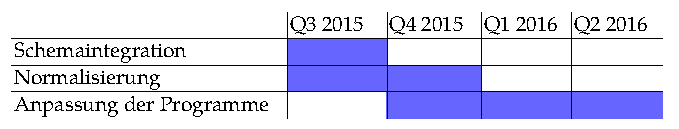
\includegraphics[width=.8\textwidth]{Abbildungen/gantt_aufwand_umsetzung_cropped.pdf}
\caption[Aufwandsschätzung Umsetzung einer teilweisen Integration von Postgres-XL]{Aufwandsschätzung Umsetzung einer teilweisen Integration von Postgres-XL in den Ist-Stand}
\label{fig:aufwand}
\end{figure}
Deshalb ist die Erstellung eines umfassenden Entwurfs hinsichtlich des speziellen Szenarios bei Agri~Con im Rahmen dieser Arbeit nicht möglich.

Der Entwurf wird daher als Klon des Ist-Standes, jedoch ohne Trigger, erstellt.
Entsprechend den Leistungstests soll der Entwurf die Produktivdaten liefern und anwendungsnahe Berechnungen ausführen.
Somit sind Aussagen zur Leistungsfähigkeit gegenüber dem Ist-Stand treffbar.
Die Speicherung von historischen Daten wird aus Zeitgründen nicht betrachtet.
Eine Übernahme aller vorhandenen Daten wurde mit Abschnitt \ref{subsection:interface} erläutert, sodass die Möglichkeit der Speicherung von historischen Daten damit gezeigt ist.

Der Ist-Stand wurde unter Kapitel \ref{IstStand} dargelegt, somit sind die Unterschiede des für die Testumgebung umgesetzten Entwurfes zu erläutern.
Das Datenbankschema unterscheidet sich von dem des Ist-Standes durch das Fehlen von Triggern und einigen Fremdschlüssel Constraints.
Diese Fremdschlüsselbeziehungen müssen entfernt werden, da Primär- und Fremdschlüssel immer in \verb+distribute by+ enthalten sein müssen, was entweder auf Grund der Stufe der Datennormalität nicht umsetzbar ist oder diese Beziehungen in den Tests nicht verwendet werden.
Diese Änderungen sind auch im Vergleichssystem mit PostgreSQL 9.3 enthalten.
Weiterhin wurden die zu testenden Funktionen an den Funktionsumfang von Postgres-XL angepasst.
Dabei wurden interne Transaktionen und inserts aus den verwendeten Funktionen entfernt.
Das Vorgehen zur Erstellung dieses Aufbaus war zusammengefasst folgender:
Postgres-XL auf sieben VMs installiert, eine Konfigurationsdatei für \verb+pgxc_ctl+ erstellt, den Cluster mit \verb+pgxc_ctl+ erzeugt, eine Datenbank mit dem Namen agrodb erzeugt, darin die Erweiterungen plr, dblink und PostGIS installiert, das Datenbankschema mit Funktionen angepasst, das Datenbankschema und Hilfsfunktionen eingespielt und die Daten mit dblink für ausgewählte Betriebe übernommen.
Die Schritte sind mit entsprechender Zeitschätzung in Abbildung \ref{fig:getan} zu finden.
\begin{figure}[h!]
\centering
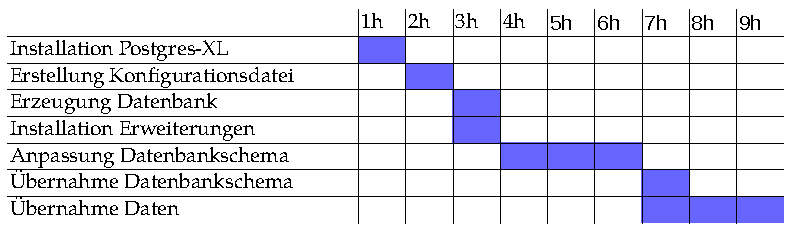
\includegraphics[width=.8\textwidth]{Abbildungen/gantt_done_cropped.pdf}
\caption[Vorgehen zur Erstellung der Postgres-XL Testumgebung]{Vorgehen zur Erstellung der Postgres-XL Testumgebung mit Zeitschätzung}
\label{fig:getan}
\end{figure}
Es handelt sich um eine Schätzung des Zeitaufwandes, da der Aufwand einzelner Schritte vom Szenario abhängt, ergo nicht allgemein bestimmbar ist.
Außerdem kann es dazu kommen, dass bei einer Fehlkonfiguration von Postgres-XL der Cluster neu erstellt werden muss, um die vollständige Umsetzung zu realisieren.\footnote{Während der Erstellung durch den Autor waren falsche Einstellungskonstellationen aus Knoten und Datenbankschema irreversibel, sodass nur eine Neuerstellung die angestrebte Konfiguration ermöglichen konnte.}

%\begin{table}[h!]
%\centering
%\small
%\begin{tabular}{l||c|c|c|c|c}
% & \textbf{Q2 2015} & \textbf{Q3 2015} & \textbf{Q4 2015} & \textbf{Q1 2016} & \textbf{Q2 2016} \\ \hline
%Teilweise Schemaintegration & \cellcolor{blue!50} & \cellcolor{blue!50} & & & \\ \hline
%Normalisierung & & {\cellcolor{blue!50}} & {\cellcolor{blue!50}} & & \\ \hline
%Anpassung der Programme & & & \cellcolor{blue!50} & \cellcolor{blue!50} & \cellcolor{blue!50} \\ 
%\end{tabular}
%\caption{}
%\label{tbl:aufwand}
%\end{table}


\chapter{Tests}
\label{chapter:tests}
%Erwartung definieren!
Postgres-XL wird hinsichtlich Funktionalität und Leistungsfähigkeit bezüglich der Anforderungen getestet.
%pgbench http://www.postgresql.org/docs/devel/static/pgbench.html
Die systematischen Tests werden in diesem Kapitel vorgestellt.
Die Kriterien wurden in Kapitel \ref{qualitätsmetriken} definiert, somit werden hier die Randbedingungen, Eingaben, Durchführung und Ergebnisse dargelegt.

\section{Testumgebung}
%verlinkungen auch zur hardware!
Die wesentliche Randbedingung Testumgebung wurde nach der Softwareauswahl und vor der Durchführung der Tests erstellt.
Die Testumgebung ist Hardware aus dem Jahr 2007 und soll dazu dienen, relative Aussagen über die Leistung von Postgres-XL zu treffen.
Dafür steht ein IBM Rack Server x3850 M2\footnote{\url{http://www.redbooks.ibm.com/redpapers/pdfs/redp4362.pdf}} mit folgender Ausstattung zur Verfügung:
vier Xeon E7330 Quad-Core mit 2,4 GHz, 64GB DDR2 RAM, vier 500GB 2,5 Zoll SATA Festplatten von Western Digital mit 7.200 U/min und einem MR10k Raid-Controller.
Der Postgres-XL Cluster wird mit Virtualisierung der einzelnen Knoten erstellt.
Als Virtualisierungssoftware kommt \Gls{esxi} in der kostenlosen Version 6.0 mit \Gls{vsphere} 6.0\footnote{\url{https://www.vmware.com/de/products/vsphere}} als Testversion zum Einsatz.
Mit dieser Virtualisierungslösung ist es möglich, Ressourcen explizit und ausschließlich einer \Gls{vm} zuzuordnen.
So werden die Prozessorkerne in Paaren und der Arbeitsspeicher direkt und mit exklusiver Verwendung den einzelnen \Gls{vm}s zugeordnet.

Ziel dieser unter Abbildung \ref{fig:physAufb} skizzierten Testumgebung ist es einen homogenen Cluster zu erzeugen und Postgres-XL mit der PostgreSQL Konfiguration des Ist Standes zu vergleichen.
% und Aussagen über die Skalierbarkeit von Postgres-XL zu treffen.

Die Ausstattung des Computers zur Verwaltung der Virtualisierung wird nicht definiert, da dies keinen Einfluss auf Messungen hat.
Die \Gls{vm}s sind in Abbildung \ref{fig:VMAufb} dargestellt.
Typ I enthält eine GTM Instanz und Typ II eine GTM-Proxy, eine Coordinator und zwei DataNode Instanzen.
Dabei stehen sechs Typ II VMs zur Verfügung.
%, wobei zur Beurteilung der Skalierbarkeit zwei bis sieben genutzt werden.
Jede \Gls{vm} besitzt als Betriebssystem Ubuntu 14.04 LTS und alle für die Installation und Ausführung des Prototypen notwendigen Pakete.
Weiterhin erhalten die Typ II \Gls{vm}s folgende Hardware Zuordnung:
zwei Prozessorkerne, sieben GB RAM und 100 GB Festplattenspeicherplatz.
Typ I erhält dagegen zwei Prozessorkerne, sieben GB RAM und 20 GB Festplattenspeicherplatz.
\begin{figure}[h!]
\centering
% Graphic for TeX using PGF
% Title: /home/tboonx/Dokumente/Studium/Masterarbeit/masterthesis/Abbildungen/Testsystem_physischerAufbau.dia
% Creator: Dia v0.97.2
% CreationDate: Sun Mar 22 16:47:12 2015
% For: tboonx
% \usepackage{tikz}
% The following commands are not supported in PSTricks at present
% We define them conditionally, so when they are implemented,
% this pgf file will use them.
\ifx\du\undefined
  \newlength{\du}
\fi
\setlength{\du}{15\unitlength}
\begin{tikzpicture}
\pgftransformxscale{1.000000}
\pgftransformyscale{-1.000000}
\definecolor{dialinecolor}{rgb}{0.000000, 0.000000, 0.000000}
\pgfsetstrokecolor{dialinecolor}
\definecolor{dialinecolor}{rgb}{1.000000, 1.000000, 1.000000}
\pgfsetfillcolor{dialinecolor}
\pgfsetlinewidth{0.100000\du}
\pgfsetdash{}{0pt}
\pgfsetdash{}{0pt}
\pgfsetbuttcap
\pgfsetmiterjoin
\pgfsetlinewidth{0.100000\du}
\pgfsetbuttcap
\pgfsetmiterjoin
\pgfsetdash{}{0pt}
\definecolor{dialinecolor}{rgb}{0.000000, 0.000000, 0.000000}
\pgfsetstrokecolor{dialinecolor}
\draw (38.088600\du,26.070243\du)--(38.088600\du,30.624686\du)--(39.606748\du,30.624686\du)--(39.606748\du,26.070243\du)--cycle;
\pgfsetlinewidth{0.010000\du}
\pgfsetbuttcap
\pgfsetmiterjoin
\pgfsetdash{}{0pt}
\definecolor{dialinecolor}{rgb}{0.000000, 0.000000, 0.000000}
\pgfsetstrokecolor{dialinecolor}
\draw (38.088600\du,26.070243\du)--(38.088600\du,30.624686\du)--(39.606748\du,30.624686\du)--(39.606748\du,26.070243\du)--cycle;
\pgfsetlinewidth{0.100000\du}
\pgfsetbuttcap
\pgfsetmiterjoin
\pgfsetdash{}{0pt}
\definecolor{dialinecolor}{rgb}{0.000000, 0.000000, 0.000000}
\pgfsetstrokecolor{dialinecolor}
\draw (38.240415\du,26.222058\du)--(38.240415\du,28.043835\du)--(39.454933\du,28.043835\du)--(39.454933\du,26.222058\du)--cycle;
\pgfsetlinewidth{0.010000\du}
\pgfsetbuttcap
\pgfsetmiterjoin
\pgfsetdash{}{0pt}
\definecolor{dialinecolor}{rgb}{0.000000, 0.000000, 0.000000}
\pgfsetstrokecolor{dialinecolor}
\draw (38.240415\du,26.222058\du)--(38.240415\du,28.043835\du)--(39.454933\du,28.043835\du)--(39.454933\du,26.222058\du)--cycle;
\pgfsetbuttcap
\pgfsetmiterjoin
\pgfsetdash{}{0pt}
\definecolor{dialinecolor}{rgb}{0.000000, 0.000000, 0.000000}
\pgfsetstrokecolor{dialinecolor}
\draw (38.240415\du,26.525688\du)--(39.454933\du,26.525688\du);
\pgfsetbuttcap
\pgfsetmiterjoin
\pgfsetdash{}{0pt}
\definecolor{dialinecolor}{rgb}{0.000000, 0.000000, 0.000000}
\pgfsetstrokecolor{dialinecolor}
\draw (39.454933\du,26.829317\du)--(38.240415\du,26.829317\du);
\pgfsetbuttcap
\pgfsetmiterjoin
\pgfsetdash{}{0pt}
\definecolor{dialinecolor}{rgb}{0.000000, 0.000000, 0.000000}
\pgfsetstrokecolor{dialinecolor}
\draw (38.240415\du,27.132947\du)--(39.454933\du,27.132947\du);
\pgfsetbuttcap
\pgfsetmiterjoin
\pgfsetdash{}{0pt}
\definecolor{dialinecolor}{rgb}{0.000000, 0.000000, 0.000000}
\pgfsetstrokecolor{dialinecolor}
\draw (38.240415\du,27.436576\du)--(39.454933\du,27.436576\du);
\pgfsetbuttcap
\pgfsetmiterjoin
\pgfsetdash{}{0pt}
\definecolor{dialinecolor}{rgb}{0.000000, 0.000000, 0.000000}
\pgfsetstrokecolor{dialinecolor}
\draw (39.454933\du,27.740206\du)--(38.240415\du,27.740206\du);
\pgfsetlinewidth{0.100000\du}
\pgfsetbuttcap
\pgfsetmiterjoin
\pgfsetdash{}{0pt}
\definecolor{dialinecolor}{rgb}{0.000000, 0.000000, 0.000000}
\pgfsetstrokecolor{dialinecolor}
\draw (38.240415\du,28.195650\du)--(38.240415\du,28.651094\du)--(39.075396\du,28.651094\du)--(39.075396\du,28.195650\du)--cycle;
\pgfsetlinewidth{0.010000\du}
\pgfsetbuttcap
\pgfsetmiterjoin
\pgfsetdash{}{0pt}
\definecolor{dialinecolor}{rgb}{0.000000, 0.000000, 0.000000}
\pgfsetstrokecolor{dialinecolor}
\draw (38.240415\du,28.195650\du)--(38.240415\du,28.651094\du)--(39.075396\du,28.651094\du)--(39.075396\du,28.195650\du)--cycle;
\pgfsetbuttcap
\pgfsetmiterjoin
\pgfsetdash{}{0pt}
\definecolor{dialinecolor}{rgb}{0.000000, 0.000000, 0.000000}
\pgfsetstrokecolor{dialinecolor}
\draw (38.088600\du,28.954724\du)--(39.606748\du,28.954724\du);
\pgfsetlinewidth{0.100000\du}
\pgfsetbuttcap
\pgfsetmiterjoin
\pgfsetdash{}{0pt}
\definecolor{dialinecolor}{rgb}{0.000000, 0.000000, 0.000000}
\pgfsetstrokecolor{dialinecolor}
\draw (38.771766\du,29.106539\du)--(38.771766\du,29.182446\du)--(38.847674\du,29.182446\du)--(38.847674\du,29.106539\du)--cycle;
\pgfsetlinewidth{0.010000\du}
\pgfsetbuttcap
\pgfsetmiterjoin
\pgfsetdash{}{0pt}
\definecolor{dialinecolor}{rgb}{0.000000, 0.000000, 0.000000}
\pgfsetstrokecolor{dialinecolor}
\draw (38.771766\du,29.106539\du)--(38.771766\du,29.182446\du)--(38.847674\du,29.182446\du)--(38.847674\du,29.106539\du)--cycle;
\pgfsetlinewidth{0.100000\du}
\pgfsetbuttcap
\pgfsetmiterjoin
\pgfsetdash{}{0pt}
\definecolor{dialinecolor}{rgb}{0.000000, 0.000000, 0.000000}
\pgfsetstrokecolor{dialinecolor}
\draw (39.075396\du,29.106539\du)--(39.075396\du,29.182446\du)--(39.151303\du,29.182446\du)--(39.151303\du,29.106539\du)--cycle;
\pgfsetlinewidth{0.010000\du}
\pgfsetbuttcap
\pgfsetmiterjoin
\pgfsetdash{}{0pt}
\definecolor{dialinecolor}{rgb}{0.000000, 0.000000, 0.000000}
\pgfsetstrokecolor{dialinecolor}
\draw (39.075396\du,29.106539\du)--(39.075396\du,29.182446\du)--(39.151303\du,29.182446\du)--(39.151303\du,29.106539\du)--cycle;
\pgfsetlinewidth{0.100000\du}
\pgfsetbuttcap
\pgfsetmiterjoin
\pgfsetdash{}{0pt}
\definecolor{dialinecolor}{rgb}{0.000000, 0.000000, 0.000000}
\pgfsetstrokecolor{dialinecolor}
\draw (39.379026\du,29.106539\du)--(39.379026\du,29.182446\du)--(39.454933\du,29.182446\du)--(39.454933\du,29.106539\du)--cycle;
\pgfsetlinewidth{0.010000\du}
\pgfsetbuttcap
\pgfsetmiterjoin
\pgfsetdash{}{0pt}
\definecolor{dialinecolor}{rgb}{0.000000, 0.000000, 0.000000}
\pgfsetstrokecolor{dialinecolor}
\draw (39.379026\du,29.106539\du)--(39.379026\du,29.182446\du)--(39.454933\du,29.182446\du)--(39.454933\du,29.106539\du)--cycle;
\pgfsetlinewidth{0.100000\du}
\pgfsetbuttcap
\pgfsetmiterjoin
\pgfsetdash{}{0pt}
\definecolor{dialinecolor}{rgb}{0.000000, 0.000000, 0.000000}
\pgfsetstrokecolor{dialinecolor}
\draw (39.303118\du,28.651094\du)--(39.303118\du,28.802909\du)--(39.454933\du,28.802909\du)--(39.454933\du,28.651094\du)--cycle;
\pgfsetlinewidth{0.010000\du}
\pgfsetbuttcap
\pgfsetmiterjoin
\pgfsetdash{}{0pt}
\definecolor{dialinecolor}{rgb}{0.000000, 0.000000, 0.000000}
\pgfsetstrokecolor{dialinecolor}
\draw (39.303118\du,28.651094\du)--(39.303118\du,28.802909\du)--(39.454933\du,28.802909\du)--(39.454933\du,28.651094\du)--cycle;
\pgfsetbuttcap
\pgfsetmiterjoin
\pgfsetdash{}{0pt}
\definecolor{dialinecolor}{rgb}{0.000000, 0.000000, 0.000000}
\pgfsetstrokecolor{dialinecolor}
\draw (38.240415\du,28.423372\du)--(39.075396\du,28.423372\du);
\pgfsetlinewidth{0.100000\du}
\pgfsetbuttcap
\pgfsetmiterjoin
\pgfsetdash{}{0pt}
\definecolor{dialinecolor}{rgb}{0.000000, 0.000000, 0.000000}
\pgfsetstrokecolor{dialinecolor}
\draw (38.240415\du,29.030631\du)--(38.240415\du,29.258353\du)--(38.468137\du,29.258353\du)--(38.468137\du,29.030631\du)--cycle;
\pgfsetlinewidth{0.010000\du}
\pgfsetbuttcap
\pgfsetmiterjoin
\pgfsetdash{}{0pt}
\definecolor{dialinecolor}{rgb}{0.000000, 0.000000, 0.000000}
\pgfsetstrokecolor{dialinecolor}
\draw (38.240415\du,29.030631\du)--(38.240415\du,29.258353\du)--(38.468137\du,29.258353\du)--(38.468137\du,29.030631\du)--cycle;
\pgfsetlinewidth{0.100000\du}
\pgfsetbuttcap
\pgfsetmiterjoin
\pgfsetdash{}{0pt}
\definecolor{dialinecolor}{rgb}{0.000000, 0.000000, 0.000000}
\pgfsetstrokecolor{dialinecolor}
\draw (38.316322\du,27.816113\du)--(38.316322\du,27.892021\du)--(39.379026\du,27.892021\du)--(39.379026\du,27.816113\du)--cycle;
\pgfsetlinewidth{0.010000\du}
\pgfsetbuttcap
\pgfsetmiterjoin
\pgfsetdash{}{0pt}
\definecolor{dialinecolor}{rgb}{0.000000, 0.000000, 0.000000}
\pgfsetstrokecolor{dialinecolor}
\draw (38.316322\du,27.816113\du)--(38.316322\du,27.892021\du)--(39.379026\du,27.892021\du)--(39.379026\du,27.816113\du)--cycle;
\pgfsetbuttcap
\pgfsetmiterjoin
\pgfsetdash{}{0pt}
\definecolor{dialinecolor}{rgb}{0.000000, 0.000000, 0.000000}
\pgfsetstrokecolor{dialinecolor}
\draw (38.316322\du,28.271557\du)--(38.999489\du,28.271557\du);
\pgfsetbuttcap
\pgfsetmiterjoin
\pgfsetdash{}{0pt}
\definecolor{dialinecolor}{rgb}{0.000000, 0.000000, 0.000000}
\pgfsetstrokecolor{dialinecolor}
\draw (38.999489\du,28.347465\du)--(38.923581\du,28.347465\du);
\pgfsetbuttcap
\pgfsetmiterjoin
\pgfsetdash{}{0pt}
\definecolor{dialinecolor}{rgb}{0.000000, 0.000000, 0.000000}
\pgfsetstrokecolor{dialinecolor}
\draw (38.316322\du,28.347465\du)--(38.392230\du,28.347465\du);
\pgfsetlinewidth{0.100000\du}
\pgfsetbuttcap
\pgfsetmiterjoin
\pgfsetdash{}{0pt}
\definecolor{dialinecolor}{rgb}{0.000000, 0.000000, 0.000000}
\pgfsetstrokecolor{dialinecolor}
\draw (38.468137\du,28.271557\du)--(38.468137\du,28.347465\du)--(38.847674\du,28.347465\du)--(38.847674\du,28.271557\du)--cycle;
\pgfsetlinewidth{0.010000\du}
\pgfsetbuttcap
\pgfsetmiterjoin
\pgfsetdash{}{0pt}
\definecolor{dialinecolor}{rgb}{0.000000, 0.000000, 0.000000}
\pgfsetstrokecolor{dialinecolor}
\draw (38.468137\du,28.271557\du)--(38.468137\du,28.347465\du)--(38.847674\du,28.347465\du)--(38.847674\du,28.271557\du)--cycle;
\pgfsetbuttcap
\pgfsetmiterjoin
\pgfsetdash{}{0pt}
\definecolor{dialinecolor}{rgb}{0.000000, 0.000000, 0.000000}
\pgfsetstrokecolor{dialinecolor}
\draw (38.316322\du,27.967928\du)--(38.392230\du,27.967928\du);
\pgfsetbuttcap
\pgfsetmiterjoin
\pgfsetdash{}{0pt}
\definecolor{dialinecolor}{rgb}{0.000000, 0.000000, 0.000000}
\pgfsetstrokecolor{dialinecolor}
\draw (38.468137\du,27.967928\du)--(38.544044\du,27.967928\du);
\pgfsetbuttcap
\pgfsetmiterjoin
\pgfsetdash{}{0pt}
\definecolor{dialinecolor}{rgb}{0.000000, 0.000000, 0.000000}
\pgfsetstrokecolor{dialinecolor}
\draw (39.227211\du,27.967928\du)--(39.379026\du,27.967928\du);
\pgfsetbuttcap
\pgfsetmiterjoin
\pgfsetdash{}{0pt}
\definecolor{dialinecolor}{rgb}{0.000000, 0.000000, 0.000000}
\pgfsetstrokecolor{dialinecolor}
\draw (38.164507\du,30.548779\du)--(39.530840\du,30.548779\du);
\pgfsetbuttcap
\pgfsetmiterjoin
\pgfsetdash{}{0pt}
\definecolor{dialinecolor}{rgb}{0.000000, 0.000000, 0.000000}
\pgfsetstrokecolor{dialinecolor}
\draw (39.530840\du,30.472872\du)--(38.164507\du,30.472872\du);
\pgfsetbuttcap
\pgfsetmiterjoin
\pgfsetdash{}{0pt}
\definecolor{dialinecolor}{rgb}{0.000000, 0.000000, 0.000000}
\pgfsetstrokecolor{dialinecolor}
\draw (38.164507\du,30.396964\du)--(39.530840\du,30.396964\du);
\pgfsetbuttcap
\pgfsetmiterjoin
\pgfsetdash{}{0pt}
\definecolor{dialinecolor}{rgb}{0.000000, 0.000000, 0.000000}
\pgfsetstrokecolor{dialinecolor}
\draw (39.530840\du,30.321057\du)--(38.164507\du,30.321057\du);
\pgfsetbuttcap
\pgfsetmiterjoin
\pgfsetdash{}{0pt}
\definecolor{dialinecolor}{rgb}{0.000000, 0.000000, 0.000000}
\pgfsetstrokecolor{dialinecolor}
\draw (38.164507\du,30.245150\du)--(39.530840\du,30.245150\du);
\pgfsetbuttcap
\pgfsetmiterjoin
\pgfsetdash{}{0pt}
\definecolor{dialinecolor}{rgb}{0.000000, 0.000000, 0.000000}
\pgfsetstrokecolor{dialinecolor}
\draw (39.530840\du,30.169242\du)--(38.164507\du,30.169242\du);
\pgfsetbuttcap
\pgfsetmiterjoin
\pgfsetdash{}{0pt}
\definecolor{dialinecolor}{rgb}{0.000000, 0.000000, 0.000000}
\pgfsetstrokecolor{dialinecolor}
\draw (38.164507\du,30.093335\du)--(39.530840\du,30.093335\du);
\pgfsetbuttcap
\pgfsetmiterjoin
\pgfsetdash{}{0pt}
\definecolor{dialinecolor}{rgb}{0.000000, 0.000000, 0.000000}
\pgfsetstrokecolor{dialinecolor}
\draw (39.530840\du,30.017427\du)--(38.164507\du,30.017427\du);
\pgfsetbuttcap
\pgfsetmiterjoin
\pgfsetdash{}{0pt}
\definecolor{dialinecolor}{rgb}{0.000000, 0.000000, 0.000000}
\pgfsetstrokecolor{dialinecolor}
\draw (38.164507\du,29.941520\du)--(39.530840\du,29.941520\du);
\pgfsetbuttcap
\pgfsetmiterjoin
\pgfsetdash{}{0pt}
\definecolor{dialinecolor}{rgb}{0.000000, 0.000000, 0.000000}
\pgfsetstrokecolor{dialinecolor}
\draw (39.530840\du,29.865613\du)--(38.164507\du,29.865613\du);
\pgfsetbuttcap
\pgfsetmiterjoin
\pgfsetdash{}{0pt}
\definecolor{dialinecolor}{rgb}{0.000000, 0.000000, 0.000000}
\pgfsetstrokecolor{dialinecolor}
\draw (38.164507\du,29.789705\du)--(39.530840\du,29.789705\du);
\pgfsetbuttcap
\pgfsetmiterjoin
\pgfsetdash{}{0pt}
\definecolor{dialinecolor}{rgb}{0.000000, 0.000000, 0.000000}
\pgfsetstrokecolor{dialinecolor}
\draw (39.530840\du,29.713798\du)--(38.164507\du,29.713798\du);
\pgfsetbuttcap
\pgfsetmiterjoin
\pgfsetdash{}{0pt}
\definecolor{dialinecolor}{rgb}{0.000000, 0.000000, 0.000000}
\pgfsetstrokecolor{dialinecolor}
\draw (38.164507\du,29.637890\du)--(39.530840\du,29.637890\du);
\pgfsetbuttcap
\pgfsetmiterjoin
\pgfsetdash{}{0pt}
\definecolor{dialinecolor}{rgb}{0.000000, 0.000000, 0.000000}
\pgfsetstrokecolor{dialinecolor}
\draw (39.530840\du,29.561983\du)--(38.164507\du,29.561983\du);
% setfont left to latex
\definecolor{dialinecolor}{rgb}{0.000000, 0.000000, 0.000000}
\pgfsetstrokecolor{dialinecolor}
\node at (38.636700\du,24.819100\du){VMware vCenter Server};
% setfont left to latex
\definecolor{dialinecolor}{rgb}{0.000000, 0.000000, 0.000000}
\pgfsetstrokecolor{dialinecolor}
\node at (38.636700\du,25.619100\du){VMware vSphere Client};
\pgfsetlinewidth{0.100000\du}
\pgfsetdash{}{0pt}
\pgfsetdash{}{0pt}
\pgfsetbuttcap
\pgfsetmiterjoin
\pgfsetlinewidth{0.100000\du}
\pgfsetbuttcap
\pgfsetmiterjoin
\pgfsetdash{}{0pt}
\definecolor{dialinecolor}{rgb}{0.000000, 0.000000, 0.000000}
\pgfsetstrokecolor{dialinecolor}
\draw (35.650000\du,34.105300\du)--(35.650000\du,35.713097\du)--(42.081186\du,35.713097\du)--(42.081186\du,34.105300\du)--cycle;
\pgfsetlinewidth{0.010000\du}
\pgfsetbuttcap
\pgfsetmiterjoin
\pgfsetdash{}{0pt}
\definecolor{dialinecolor}{rgb}{0.000000, 0.000000, 0.000000}
\pgfsetstrokecolor{dialinecolor}
\draw (35.650000\du,34.105300\du)--(35.650000\du,35.713097\du)--(42.081186\du,35.713097\du)--(42.081186\du,34.105300\du)--cycle;
\pgfsetbuttcap
\pgfsetmiterjoin
\pgfsetdash{}{0pt}
\definecolor{dialinecolor}{rgb}{0.000000, 0.000000, 0.000000}
\pgfsetstrokecolor{dialinecolor}
\draw (36.775458\du,34.748419\du)--(36.614678\du,34.909198\du);
\pgfsetbuttcap
\pgfsetmiterjoin
\pgfsetdash{}{0pt}
\definecolor{dialinecolor}{rgb}{0.000000, 0.000000, 0.000000}
\pgfsetstrokecolor{dialinecolor}
\draw (36.614678\du,34.909198\du)--(36.775458\du,35.069978\du);
\pgfsetbuttcap
\pgfsetmiterjoin
\pgfsetdash{}{0pt}
\definecolor{dialinecolor}{rgb}{0.000000, 0.000000, 0.000000}
\pgfsetstrokecolor{dialinecolor}
\draw (37.418576\du,34.748419\du)--(37.257797\du,34.909198\du);
\pgfsetbuttcap
\pgfsetmiterjoin
\pgfsetdash{}{0pt}
\definecolor{dialinecolor}{rgb}{0.000000, 0.000000, 0.000000}
\pgfsetstrokecolor{dialinecolor}
\draw (37.257797\du,34.909198\du)--(37.418576\du,35.069978\du);
\pgfsetbuttcap
\pgfsetmiterjoin
\pgfsetdash{}{0pt}
\definecolor{dialinecolor}{rgb}{0.000000, 0.000000, 0.000000}
\pgfsetstrokecolor{dialinecolor}
\draw (38.061695\du,34.748419\du)--(37.900915\du,34.909198\du);
\pgfsetbuttcap
\pgfsetmiterjoin
\pgfsetdash{}{0pt}
\definecolor{dialinecolor}{rgb}{0.000000, 0.000000, 0.000000}
\pgfsetstrokecolor{dialinecolor}
\draw (37.900915\du,34.909198\du)--(38.061695\du,35.069978\du);
\pgfsetbuttcap
\pgfsetmiterjoin
\pgfsetdash{}{0pt}
\definecolor{dialinecolor}{rgb}{0.000000, 0.000000, 0.000000}
\pgfsetstrokecolor{dialinecolor}
\draw (38.704814\du,34.748419\du)--(38.544034\du,34.909198\du);
\pgfsetbuttcap
\pgfsetmiterjoin
\pgfsetdash{}{0pt}
\definecolor{dialinecolor}{rgb}{0.000000, 0.000000, 0.000000}
\pgfsetstrokecolor{dialinecolor}
\draw (38.544034\du,34.909198\du)--(38.704814\du,35.069978\du);
\pgfsetbuttcap
\pgfsetmiterjoin
\pgfsetdash{}{0pt}
\definecolor{dialinecolor}{rgb}{0.000000, 0.000000, 0.000000}
\pgfsetstrokecolor{dialinecolor}
\draw (39.347932\du,34.748419\du)--(39.187153\du,34.909198\du);
\pgfsetbuttcap
\pgfsetmiterjoin
\pgfsetdash{}{0pt}
\definecolor{dialinecolor}{rgb}{0.000000, 0.000000, 0.000000}
\pgfsetstrokecolor{dialinecolor}
\draw (39.187153\du,34.909198\du)--(39.347932\du,35.069978\du);
\pgfsetbuttcap
\pgfsetmiterjoin
\pgfsetdash{}{0pt}
\definecolor{dialinecolor}{rgb}{0.000000, 0.000000, 0.000000}
\pgfsetstrokecolor{dialinecolor}
\draw (39.991051\du,34.748419\du)--(39.830271\du,34.909198\du);
\pgfsetbuttcap
\pgfsetmiterjoin
\pgfsetdash{}{0pt}
\definecolor{dialinecolor}{rgb}{0.000000, 0.000000, 0.000000}
\pgfsetstrokecolor{dialinecolor}
\draw (39.830271\du,34.909198\du)--(39.991051\du,35.069978\du);
\pgfsetbuttcap
\pgfsetmiterjoin
\pgfsetdash{}{0pt}
\definecolor{dialinecolor}{rgb}{0.000000, 0.000000, 0.000000}
\pgfsetstrokecolor{dialinecolor}
\draw (40.634170\du,34.748419\du)--(40.473390\du,34.909198\du);
\pgfsetbuttcap
\pgfsetmiterjoin
\pgfsetdash{}{0pt}
\definecolor{dialinecolor}{rgb}{0.000000, 0.000000, 0.000000}
\pgfsetstrokecolor{dialinecolor}
\draw (40.473390\du,34.909198\du)--(40.634170\du,35.069978\du);
\pgfsetbuttcap
\pgfsetmiterjoin
\pgfsetdash{}{0pt}
\definecolor{dialinecolor}{rgb}{0.000000, 0.000000, 0.000000}
\pgfsetstrokecolor{dialinecolor}
\draw (41.277288\du,34.748419\du)--(41.116509\du,34.909198\du);
\pgfsetbuttcap
\pgfsetmiterjoin
\pgfsetdash{}{0pt}
\definecolor{dialinecolor}{rgb}{0.000000, 0.000000, 0.000000}
\pgfsetstrokecolor{dialinecolor}
\draw (41.116509\du,34.909198\du)--(41.277288\du,35.069978\du);
\pgfsetbuttcap
\pgfsetmiterjoin
\pgfsetdash{}{0pt}
\definecolor{dialinecolor}{rgb}{0.000000, 0.000000, 0.000000}
\pgfsetstrokecolor{dialinecolor}
\draw (41.598847\du,35.230758\du)--(41.438068\du,35.391537\du);
\pgfsetbuttcap
\pgfsetmiterjoin
\pgfsetdash{}{0pt}
\definecolor{dialinecolor}{rgb}{0.000000, 0.000000, 0.000000}
\pgfsetstrokecolor{dialinecolor}
\draw (41.438068\du,35.391537\du)--(41.598847\du,35.552317\du);
\pgfsetbuttcap
\pgfsetmiterjoin
\pgfsetdash{}{0pt}
\definecolor{dialinecolor}{rgb}{0.000000, 0.000000, 0.000000}
\pgfsetstrokecolor{dialinecolor}
\draw (40.955729\du,35.230758\du)--(40.794949\du,35.391537\du);
\pgfsetbuttcap
\pgfsetmiterjoin
\pgfsetdash{}{0pt}
\definecolor{dialinecolor}{rgb}{0.000000, 0.000000, 0.000000}
\pgfsetstrokecolor{dialinecolor}
\draw (40.794949\du,35.391537\du)--(40.955729\du,35.552317\du);
\pgfsetbuttcap
\pgfsetmiterjoin
\pgfsetdash{}{0pt}
\definecolor{dialinecolor}{rgb}{0.000000, 0.000000, 0.000000}
\pgfsetstrokecolor{dialinecolor}
\draw (40.312610\du,35.230758\du)--(40.151831\du,35.391537\du);
\pgfsetbuttcap
\pgfsetmiterjoin
\pgfsetdash{}{0pt}
\definecolor{dialinecolor}{rgb}{0.000000, 0.000000, 0.000000}
\pgfsetstrokecolor{dialinecolor}
\draw (40.151831\du,35.391537\du)--(40.312610\du,35.552317\du);
\pgfsetbuttcap
\pgfsetmiterjoin
\pgfsetdash{}{0pt}
\definecolor{dialinecolor}{rgb}{0.000000, 0.000000, 0.000000}
\pgfsetstrokecolor{dialinecolor}
\draw (39.669492\du,35.230758\du)--(39.508712\du,35.391537\du);
\pgfsetbuttcap
\pgfsetmiterjoin
\pgfsetdash{}{0pt}
\definecolor{dialinecolor}{rgb}{0.000000, 0.000000, 0.000000}
\pgfsetstrokecolor{dialinecolor}
\draw (39.508712\du,35.391537\du)--(39.669492\du,35.552317\du);
\pgfsetbuttcap
\pgfsetmiterjoin
\pgfsetdash{}{0pt}
\definecolor{dialinecolor}{rgb}{0.000000, 0.000000, 0.000000}
\pgfsetstrokecolor{dialinecolor}
\draw (39.026373\du,35.230758\du)--(38.865593\du,35.391537\du);
\pgfsetbuttcap
\pgfsetmiterjoin
\pgfsetdash{}{0pt}
\definecolor{dialinecolor}{rgb}{0.000000, 0.000000, 0.000000}
\pgfsetstrokecolor{dialinecolor}
\draw (38.865593\du,35.391537\du)--(39.026373\du,35.552317\du);
\pgfsetbuttcap
\pgfsetmiterjoin
\pgfsetdash{}{0pt}
\definecolor{dialinecolor}{rgb}{0.000000, 0.000000, 0.000000}
\pgfsetstrokecolor{dialinecolor}
\draw (38.383254\du,35.230758\du)--(38.222475\du,35.391537\du);
\pgfsetbuttcap
\pgfsetmiterjoin
\pgfsetdash{}{0pt}
\definecolor{dialinecolor}{rgb}{0.000000, 0.000000, 0.000000}
\pgfsetstrokecolor{dialinecolor}
\draw (38.222475\du,35.391537\du)--(38.383254\du,35.552317\du);
\pgfsetbuttcap
\pgfsetmiterjoin
\pgfsetdash{}{0pt}
\definecolor{dialinecolor}{rgb}{0.000000, 0.000000, 0.000000}
\pgfsetstrokecolor{dialinecolor}
\draw (37.740136\du,35.230758\du)--(37.579356\du,35.391537\du);
\pgfsetbuttcap
\pgfsetmiterjoin
\pgfsetdash{}{0pt}
\definecolor{dialinecolor}{rgb}{0.000000, 0.000000, 0.000000}
\pgfsetstrokecolor{dialinecolor}
\draw (37.579356\du,35.391537\du)--(37.740136\du,35.552317\du);
\pgfsetlinewidth{0.100000\du}
\pgfsetbuttcap
\pgfsetmiterjoin
\pgfsetdash{}{0pt}
\definecolor{dialinecolor}{rgb}{0.000000, 0.000000, 0.000000}
\pgfsetstrokecolor{dialinecolor}
\draw (36.775458\du,35.391537\du)--(36.775458\du,35.552317\du)--(37.418576\du,35.552317\du)--(37.418576\du,35.391537\du)--cycle;
\pgfsetlinewidth{0.010000\du}
\pgfsetbuttcap
\pgfsetmiterjoin
\pgfsetdash{}{0pt}
\definecolor{dialinecolor}{rgb}{0.000000, 0.000000, 0.000000}
\pgfsetstrokecolor{dialinecolor}
\draw (36.775458\du,35.391537\du)--(36.775458\du,35.552317\du)--(37.418576\du,35.552317\du)--(37.418576\du,35.391537\du)--cycle;
\pgfsetlinewidth{0.100000\du}
\pgfsetbuttcap
\pgfsetmiterjoin
\pgfsetdash{}{0pt}
\definecolor{dialinecolor}{rgb}{0.000000, 0.000000, 0.000000}
\pgfsetstrokecolor{dialinecolor}
\draw (36.132339\du,34.909198\du)--(36.453898\du,35.230758\du)--(36.132339\du,35.552317\du)--(35.810780\du,35.230758\du)--cycle;
\pgfsetlinewidth{0.010000\du}
\pgfsetbuttcap
\pgfsetmiterjoin
\pgfsetdash{}{0pt}
\definecolor{dialinecolor}{rgb}{0.000000, 0.000000, 0.000000}
\pgfsetstrokecolor{dialinecolor}
\draw (36.132339\du,34.909198\du)--(36.453898\du,35.230758\du)--(36.132339\du,35.552317\du)--(35.810780\du,35.230758\du)--cycle;
\pgfsetlinewidth{0.100000\du}
\pgfsetbuttcap
\pgfsetmiterjoin
\pgfsetdash{}{0pt}
\definecolor{dialinecolor}{rgb}{0.000000, 0.000000, 0.000000}
\pgfsetstrokecolor{dialinecolor}
\draw (35.650000\du,34.426859\du)--(35.650000\du,34.587639\du)--(42.081186\du,34.587639\du)--(42.081186\du,34.426859\du)--cycle;
\pgfsetlinewidth{0.010000\du}
\pgfsetbuttcap
\pgfsetmiterjoin
\pgfsetdash{}{0pt}
\definecolor{dialinecolor}{rgb}{0.000000, 0.000000, 0.000000}
\pgfsetstrokecolor{dialinecolor}
\draw (35.650000\du,34.426859\du)--(35.650000\du,34.587639\du)--(42.081186\du,34.587639\du)--(42.081186\du,34.426859\du)--cycle;
\pgfsetlinewidth{0.100000\du}
\pgfsetbuttcap
\pgfsetmiterjoin
\pgfsetdash{}{0pt}
\definecolor{dialinecolor}{rgb}{0.000000, 0.000000, 0.000000}
\pgfsetstrokecolor{dialinecolor}
\draw (36.453898\du,34.426859\du)--(36.453898\du,34.587639\du)--(37.900915\du,34.587639\du)--(37.900915\du,34.426859\du)--cycle;
\pgfsetlinewidth{0.010000\du}
\pgfsetbuttcap
\pgfsetmiterjoin
\pgfsetdash{}{0pt}
\definecolor{dialinecolor}{rgb}{0.000000, 0.000000, 0.000000}
\pgfsetstrokecolor{dialinecolor}
\draw (36.453898\du,34.426859\du)--(36.453898\du,34.587639\du)--(37.900915\du,34.587639\du)--(37.900915\du,34.426859\du)--cycle;
% setfont left to latex
\definecolor{dialinecolor}{rgb}{0.000000, 0.000000, 0.000000}
\pgfsetstrokecolor{dialinecolor}
\node at (39.078800\du,36.378000\du){IBM RackServer};
% setfont left to latex
\definecolor{dialinecolor}{rgb}{0.000000, 0.000000, 0.000000}
\pgfsetstrokecolor{dialinecolor}
\node at (39.078800\du,37.178000\du){VMware ESXi};
\pgfsetlinewidth{0.100000\du}
\pgfsetdash{}{0pt}
\pgfsetdash{}{0pt}
\pgfsetbuttcap
{
\definecolor{dialinecolor}{rgb}{0.000000, 0.000000, 0.000000}
\pgfsetfillcolor{dialinecolor}
% was here!!!
\pgfsetarrowsstart{latex}
\pgfsetarrowsend{latex}
\definecolor{dialinecolor}{rgb}{0.000000, 0.000000, 0.000000}
\pgfsetstrokecolor{dialinecolor}
\draw (38.847674\du,30.624686\du)--(38.865593\du,34.105300\du);
}
% setfont left to latex
\definecolor{dialinecolor}{rgb}{0.000000, 0.000000, 0.000000}
\pgfsetstrokecolor{dialinecolor}
\node[anchor=west] at (38.959000\du,32.514900\du){Ethernet};
\end{tikzpicture}

\caption[Aufbau der Geräte des Testsystems]{Aufbau der Geräte des Testsystems}
\label{fig:physAufb}
\end{figure}
\begin{figure}[h!]
\centering
% Graphic for TeX using PGF
% Title: /home/tboonx/Dokumente/Studium/Masterarbeit/masterthesis/Abbildungen/Testsystem_VMs.dia
% Creator: Dia v0.97.2
% CreationDate: Thu Apr 23 17:29:28 2015
% For: tboonx
% \usepackage{tikz}
% The following commands are not supported in PSTricks at present
% We define them conditionally, so when they are implemented,
% this pgf file will use them.
\ifx\du\undefined
  \newlength{\du}
\fi
\setlength{\du}{15\unitlength}
\begin{tikzpicture}
\pgftransformxscale{1.000000}
\pgftransformyscale{-1.000000}
\definecolor{dialinecolor}{rgb}{0.000000, 0.000000, 0.000000}
\pgfsetstrokecolor{dialinecolor}
\definecolor{dialinecolor}{rgb}{1.000000, 1.000000, 1.000000}
\pgfsetfillcolor{dialinecolor}
\pgfsetlinewidth{0.100000\du}
\pgfsetdash{}{0pt}
\pgfsetdash{}{0pt}
\pgfsetmiterjoin
\pgfsetbuttcap
\definecolor{dialinecolor}{rgb}{0.000000, 0.000000, 0.000000}
\pgfsetstrokecolor{dialinecolor}
\draw (48.300000\du,24.162500\du)--(53.200000\du,24.212500\du)--(53.150000\du,26.712500\du)--(55.550000\du,26.762500\du)--(55.550000\du,35.162500\du)--(46.050000\du,35.112500\du)--(46.100000\du,26.862500\du)--(48.350000\du,26.862500\du)--cycle;
\pgfsetlinewidth{0.100000\du}
\pgfsetdash{}{0pt}
\pgfsetdash{}{0pt}
\pgfsetbuttcap
\pgfsetmiterjoin
\pgfsetlinewidth{0.100000\du}
\pgfsetbuttcap
\pgfsetmiterjoin
\pgfsetdash{}{0pt}
\definecolor{dialinecolor}{rgb}{0.000000, 0.000000, 0.000000}
\pgfsetstrokecolor{dialinecolor}
\draw (48.874800\du,24.869200\du)--(48.874800\du,25.775015\du)--(52.498061\du,25.775015\du)--(52.498061\du,24.869200\du)--cycle;
\pgfsetlinewidth{0.010000\du}
\pgfsetbuttcap
\pgfsetmiterjoin
\pgfsetdash{}{0pt}
\definecolor{dialinecolor}{rgb}{0.000000, 0.000000, 0.000000}
\pgfsetstrokecolor{dialinecolor}
\draw (48.874800\du,24.869200\du)--(48.874800\du,25.775015\du)--(52.498061\du,25.775015\du)--(52.498061\du,24.869200\du)--cycle;
\pgfsetbuttcap
\pgfsetmiterjoin
\pgfsetdash{}{0pt}
\definecolor{dialinecolor}{rgb}{0.000000, 0.000000, 0.000000}
\pgfsetstrokecolor{dialinecolor}
\draw (49.508871\du,25.231526\du)--(49.418289\du,25.322108\du);
\pgfsetbuttcap
\pgfsetmiterjoin
\pgfsetdash{}{0pt}
\definecolor{dialinecolor}{rgb}{0.000000, 0.000000, 0.000000}
\pgfsetstrokecolor{dialinecolor}
\draw (49.418289\du,25.322108\du)--(49.508871\du,25.412689\du);
\pgfsetbuttcap
\pgfsetmiterjoin
\pgfsetdash{}{0pt}
\definecolor{dialinecolor}{rgb}{0.000000, 0.000000, 0.000000}
\pgfsetstrokecolor{dialinecolor}
\draw (49.871197\du,25.231526\du)--(49.780615\du,25.322108\du);
\pgfsetbuttcap
\pgfsetmiterjoin
\pgfsetdash{}{0pt}
\definecolor{dialinecolor}{rgb}{0.000000, 0.000000, 0.000000}
\pgfsetstrokecolor{dialinecolor}
\draw (49.780615\du,25.322108\du)--(49.871197\du,25.412689\du);
\pgfsetbuttcap
\pgfsetmiterjoin
\pgfsetdash{}{0pt}
\definecolor{dialinecolor}{rgb}{0.000000, 0.000000, 0.000000}
\pgfsetstrokecolor{dialinecolor}
\draw (50.233523\du,25.231526\du)--(50.142941\du,25.322108\du);
\pgfsetbuttcap
\pgfsetmiterjoin
\pgfsetdash{}{0pt}
\definecolor{dialinecolor}{rgb}{0.000000, 0.000000, 0.000000}
\pgfsetstrokecolor{dialinecolor}
\draw (50.142941\du,25.322108\du)--(50.233523\du,25.412689\du);
\pgfsetbuttcap
\pgfsetmiterjoin
\pgfsetdash{}{0pt}
\definecolor{dialinecolor}{rgb}{0.000000, 0.000000, 0.000000}
\pgfsetstrokecolor{dialinecolor}
\draw (50.595849\du,25.231526\du)--(50.505268\du,25.322108\du);
\pgfsetbuttcap
\pgfsetmiterjoin
\pgfsetdash{}{0pt}
\definecolor{dialinecolor}{rgb}{0.000000, 0.000000, 0.000000}
\pgfsetstrokecolor{dialinecolor}
\draw (50.505268\du,25.322108\du)--(50.595849\du,25.412689\du);
\pgfsetbuttcap
\pgfsetmiterjoin
\pgfsetdash{}{0pt}
\definecolor{dialinecolor}{rgb}{0.000000, 0.000000, 0.000000}
\pgfsetstrokecolor{dialinecolor}
\draw (50.958175\du,25.231526\du)--(50.867594\du,25.322108\du);
\pgfsetbuttcap
\pgfsetmiterjoin
\pgfsetdash{}{0pt}
\definecolor{dialinecolor}{rgb}{0.000000, 0.000000, 0.000000}
\pgfsetstrokecolor{dialinecolor}
\draw (50.867594\du,25.322108\du)--(50.958175\du,25.412689\du);
\pgfsetbuttcap
\pgfsetmiterjoin
\pgfsetdash{}{0pt}
\definecolor{dialinecolor}{rgb}{0.000000, 0.000000, 0.000000}
\pgfsetstrokecolor{dialinecolor}
\draw (51.320501\du,25.231526\du)--(51.229920\du,25.322108\du);
\pgfsetbuttcap
\pgfsetmiterjoin
\pgfsetdash{}{0pt}
\definecolor{dialinecolor}{rgb}{0.000000, 0.000000, 0.000000}
\pgfsetstrokecolor{dialinecolor}
\draw (51.229920\du,25.322108\du)--(51.320501\du,25.412689\du);
\pgfsetbuttcap
\pgfsetmiterjoin
\pgfsetdash{}{0pt}
\definecolor{dialinecolor}{rgb}{0.000000, 0.000000, 0.000000}
\pgfsetstrokecolor{dialinecolor}
\draw (51.682827\du,25.231526\du)--(51.592246\du,25.322108\du);
\pgfsetbuttcap
\pgfsetmiterjoin
\pgfsetdash{}{0pt}
\definecolor{dialinecolor}{rgb}{0.000000, 0.000000, 0.000000}
\pgfsetstrokecolor{dialinecolor}
\draw (51.592246\du,25.322108\du)--(51.682827\du,25.412689\du);
\pgfsetbuttcap
\pgfsetmiterjoin
\pgfsetdash{}{0pt}
\definecolor{dialinecolor}{rgb}{0.000000, 0.000000, 0.000000}
\pgfsetstrokecolor{dialinecolor}
\draw (52.045154\du,25.231526\du)--(51.954572\du,25.322108\du);
\pgfsetbuttcap
\pgfsetmiterjoin
\pgfsetdash{}{0pt}
\definecolor{dialinecolor}{rgb}{0.000000, 0.000000, 0.000000}
\pgfsetstrokecolor{dialinecolor}
\draw (51.954572\du,25.322108\du)--(52.045154\du,25.412689\du);
\pgfsetbuttcap
\pgfsetmiterjoin
\pgfsetdash{}{0pt}
\definecolor{dialinecolor}{rgb}{0.000000, 0.000000, 0.000000}
\pgfsetstrokecolor{dialinecolor}
\draw (52.226317\du,25.503271\du)--(52.135735\du,25.593852\du);
\pgfsetbuttcap
\pgfsetmiterjoin
\pgfsetdash{}{0pt}
\definecolor{dialinecolor}{rgb}{0.000000, 0.000000, 0.000000}
\pgfsetstrokecolor{dialinecolor}
\draw (52.135735\du,25.593852\du)--(52.226317\du,25.684434\du);
\pgfsetbuttcap
\pgfsetmiterjoin
\pgfsetdash{}{0pt}
\definecolor{dialinecolor}{rgb}{0.000000, 0.000000, 0.000000}
\pgfsetstrokecolor{dialinecolor}
\draw (51.863990\du,25.503271\du)--(51.773409\du,25.593852\du);
\pgfsetbuttcap
\pgfsetmiterjoin
\pgfsetdash{}{0pt}
\definecolor{dialinecolor}{rgb}{0.000000, 0.000000, 0.000000}
\pgfsetstrokecolor{dialinecolor}
\draw (51.773409\du,25.593852\du)--(51.863990\du,25.684434\du);
\pgfsetbuttcap
\pgfsetmiterjoin
\pgfsetdash{}{0pt}
\definecolor{dialinecolor}{rgb}{0.000000, 0.000000, 0.000000}
\pgfsetstrokecolor{dialinecolor}
\draw (51.501664\du,25.503271\du)--(51.411083\du,25.593852\du);
\pgfsetbuttcap
\pgfsetmiterjoin
\pgfsetdash{}{0pt}
\definecolor{dialinecolor}{rgb}{0.000000, 0.000000, 0.000000}
\pgfsetstrokecolor{dialinecolor}
\draw (51.411083\du,25.593852\du)--(51.501664\du,25.684434\du);
\pgfsetbuttcap
\pgfsetmiterjoin
\pgfsetdash{}{0pt}
\definecolor{dialinecolor}{rgb}{0.000000, 0.000000, 0.000000}
\pgfsetstrokecolor{dialinecolor}
\draw (51.139338\du,25.503271\du)--(51.048757\du,25.593852\du);
\pgfsetbuttcap
\pgfsetmiterjoin
\pgfsetdash{}{0pt}
\definecolor{dialinecolor}{rgb}{0.000000, 0.000000, 0.000000}
\pgfsetstrokecolor{dialinecolor}
\draw (51.048757\du,25.593852\du)--(51.139338\du,25.684434\du);
\pgfsetbuttcap
\pgfsetmiterjoin
\pgfsetdash{}{0pt}
\definecolor{dialinecolor}{rgb}{0.000000, 0.000000, 0.000000}
\pgfsetstrokecolor{dialinecolor}
\draw (50.777012\du,25.503271\du)--(50.686431\du,25.593852\du);
\pgfsetbuttcap
\pgfsetmiterjoin
\pgfsetdash{}{0pt}
\definecolor{dialinecolor}{rgb}{0.000000, 0.000000, 0.000000}
\pgfsetstrokecolor{dialinecolor}
\draw (50.686431\du,25.593852\du)--(50.777012\du,25.684434\du);
\pgfsetbuttcap
\pgfsetmiterjoin
\pgfsetdash{}{0pt}
\definecolor{dialinecolor}{rgb}{0.000000, 0.000000, 0.000000}
\pgfsetstrokecolor{dialinecolor}
\draw (50.414686\du,25.503271\du)--(50.324104\du,25.593852\du);
\pgfsetbuttcap
\pgfsetmiterjoin
\pgfsetdash{}{0pt}
\definecolor{dialinecolor}{rgb}{0.000000, 0.000000, 0.000000}
\pgfsetstrokecolor{dialinecolor}
\draw (50.324104\du,25.593852\du)--(50.414686\du,25.684434\du);
\pgfsetbuttcap
\pgfsetmiterjoin
\pgfsetdash{}{0pt}
\definecolor{dialinecolor}{rgb}{0.000000, 0.000000, 0.000000}
\pgfsetstrokecolor{dialinecolor}
\draw (50.052360\du,25.503271\du)--(49.961778\du,25.593852\du);
\pgfsetbuttcap
\pgfsetmiterjoin
\pgfsetdash{}{0pt}
\definecolor{dialinecolor}{rgb}{0.000000, 0.000000, 0.000000}
\pgfsetstrokecolor{dialinecolor}
\draw (49.961778\du,25.593852\du)--(50.052360\du,25.684434\du);
\pgfsetlinewidth{0.100000\du}
\pgfsetbuttcap
\pgfsetmiterjoin
\pgfsetdash{}{0pt}
\definecolor{dialinecolor}{rgb}{0.000000, 0.000000, 0.000000}
\pgfsetstrokecolor{dialinecolor}
\draw (49.508871\du,25.593852\du)--(49.508871\du,25.684434\du)--(49.871197\du,25.684434\du)--(49.871197\du,25.593852\du)--cycle;
\pgfsetlinewidth{0.010000\du}
\pgfsetbuttcap
\pgfsetmiterjoin
\pgfsetdash{}{0pt}
\definecolor{dialinecolor}{rgb}{0.000000, 0.000000, 0.000000}
\pgfsetstrokecolor{dialinecolor}
\draw (49.508871\du,25.593852\du)--(49.508871\du,25.684434\du)--(49.871197\du,25.684434\du)--(49.871197\du,25.593852\du)--cycle;
\pgfsetlinewidth{0.100000\du}
\pgfsetbuttcap
\pgfsetmiterjoin
\pgfsetdash{}{0pt}
\definecolor{dialinecolor}{rgb}{0.000000, 0.000000, 0.000000}
\pgfsetstrokecolor{dialinecolor}
\draw (49.146545\du,25.322108\du)--(49.327708\du,25.503271\du)--(49.146545\du,25.684434\du)--(48.965382\du,25.503271\du)--cycle;
\pgfsetlinewidth{0.010000\du}
\pgfsetbuttcap
\pgfsetmiterjoin
\pgfsetdash{}{0pt}
\definecolor{dialinecolor}{rgb}{0.000000, 0.000000, 0.000000}
\pgfsetstrokecolor{dialinecolor}
\draw (49.146545\du,25.322108\du)--(49.327708\du,25.503271\du)--(49.146545\du,25.684434\du)--(48.965382\du,25.503271\du)--cycle;
\pgfsetlinewidth{0.100000\du}
\pgfsetbuttcap
\pgfsetmiterjoin
\pgfsetdash{}{0pt}
\definecolor{dialinecolor}{rgb}{0.000000, 0.000000, 0.000000}
\pgfsetstrokecolor{dialinecolor}
\draw (48.874800\du,25.050363\du)--(48.874800\du,25.140945\du)--(52.498061\du,25.140945\du)--(52.498061\du,25.050363\du)--cycle;
\pgfsetlinewidth{0.010000\du}
\pgfsetbuttcap
\pgfsetmiterjoin
\pgfsetdash{}{0pt}
\definecolor{dialinecolor}{rgb}{0.000000, 0.000000, 0.000000}
\pgfsetstrokecolor{dialinecolor}
\draw (48.874800\du,25.050363\du)--(48.874800\du,25.140945\du)--(52.498061\du,25.140945\du)--(52.498061\du,25.050363\du)--cycle;
\pgfsetlinewidth{0.100000\du}
\pgfsetbuttcap
\pgfsetmiterjoin
\pgfsetdash{}{0pt}
\definecolor{dialinecolor}{rgb}{0.000000, 0.000000, 0.000000}
\pgfsetstrokecolor{dialinecolor}
\draw (49.327708\du,25.050363\du)--(49.327708\du,25.140945\du)--(50.142941\du,25.140945\du)--(50.142941\du,25.050363\du)--cycle;
\pgfsetlinewidth{0.010000\du}
\pgfsetbuttcap
\pgfsetmiterjoin
\pgfsetdash{}{0pt}
\definecolor{dialinecolor}{rgb}{0.000000, 0.000000, 0.000000}
\pgfsetstrokecolor{dialinecolor}
\draw (49.327708\du,25.050363\du)--(49.327708\du,25.140945\du)--(50.142941\du,25.140945\du)--(50.142941\du,25.050363\du)--cycle;
% setfont left to latex
\definecolor{dialinecolor}{rgb}{0.000000, 0.000000, 0.000000}
\pgfsetstrokecolor{dialinecolor}
\node[anchor=west] at (48.826600\du,26.545700\du){Typ I};
\pgfsetlinewidth{0.100000\du}
\pgfsetdash{}{0pt}
\pgfsetdash{}{0pt}
\pgfsetbuttcap
\pgfsetmiterjoin
\pgfsetlinewidth{0.100000\du}
\pgfsetbuttcap
\pgfsetmiterjoin
\pgfsetdash{}{0pt}
\definecolor{dialinecolor}{rgb}{0.000000, 0.000000, 0.000000}
\pgfsetstrokecolor{dialinecolor}
\draw (46.742100\du,27.647500\du)--(46.742100\du,28.553315\du)--(50.365361\du,28.553315\du)--(50.365361\du,27.647500\du)--cycle;
\pgfsetlinewidth{0.010000\du}
\pgfsetbuttcap
\pgfsetmiterjoin
\pgfsetdash{}{0pt}
\definecolor{dialinecolor}{rgb}{0.000000, 0.000000, 0.000000}
\pgfsetstrokecolor{dialinecolor}
\draw (46.742100\du,27.647500\du)--(46.742100\du,28.553315\du)--(50.365361\du,28.553315\du)--(50.365361\du,27.647500\du)--cycle;
\pgfsetbuttcap
\pgfsetmiterjoin
\pgfsetdash{}{0pt}
\definecolor{dialinecolor}{rgb}{0.000000, 0.000000, 0.000000}
\pgfsetstrokecolor{dialinecolor}
\draw (47.376171\du,28.009826\du)--(47.285589\du,28.100408\du);
\pgfsetbuttcap
\pgfsetmiterjoin
\pgfsetdash{}{0pt}
\definecolor{dialinecolor}{rgb}{0.000000, 0.000000, 0.000000}
\pgfsetstrokecolor{dialinecolor}
\draw (47.285589\du,28.100408\du)--(47.376171\du,28.190989\du);
\pgfsetbuttcap
\pgfsetmiterjoin
\pgfsetdash{}{0pt}
\definecolor{dialinecolor}{rgb}{0.000000, 0.000000, 0.000000}
\pgfsetstrokecolor{dialinecolor}
\draw (47.738497\du,28.009826\du)--(47.647915\du,28.100408\du);
\pgfsetbuttcap
\pgfsetmiterjoin
\pgfsetdash{}{0pt}
\definecolor{dialinecolor}{rgb}{0.000000, 0.000000, 0.000000}
\pgfsetstrokecolor{dialinecolor}
\draw (47.647915\du,28.100408\du)--(47.738497\du,28.190989\du);
\pgfsetbuttcap
\pgfsetmiterjoin
\pgfsetdash{}{0pt}
\definecolor{dialinecolor}{rgb}{0.000000, 0.000000, 0.000000}
\pgfsetstrokecolor{dialinecolor}
\draw (48.100823\du,28.009826\du)--(48.010241\du,28.100408\du);
\pgfsetbuttcap
\pgfsetmiterjoin
\pgfsetdash{}{0pt}
\definecolor{dialinecolor}{rgb}{0.000000, 0.000000, 0.000000}
\pgfsetstrokecolor{dialinecolor}
\draw (48.010241\du,28.100408\du)--(48.100823\du,28.190989\du);
\pgfsetbuttcap
\pgfsetmiterjoin
\pgfsetdash{}{0pt}
\definecolor{dialinecolor}{rgb}{0.000000, 0.000000, 0.000000}
\pgfsetstrokecolor{dialinecolor}
\draw (48.463149\du,28.009826\du)--(48.372568\du,28.100408\du);
\pgfsetbuttcap
\pgfsetmiterjoin
\pgfsetdash{}{0pt}
\definecolor{dialinecolor}{rgb}{0.000000, 0.000000, 0.000000}
\pgfsetstrokecolor{dialinecolor}
\draw (48.372568\du,28.100408\du)--(48.463149\du,28.190989\du);
\pgfsetbuttcap
\pgfsetmiterjoin
\pgfsetdash{}{0pt}
\definecolor{dialinecolor}{rgb}{0.000000, 0.000000, 0.000000}
\pgfsetstrokecolor{dialinecolor}
\draw (48.825475\du,28.009826\du)--(48.734894\du,28.100408\du);
\pgfsetbuttcap
\pgfsetmiterjoin
\pgfsetdash{}{0pt}
\definecolor{dialinecolor}{rgb}{0.000000, 0.000000, 0.000000}
\pgfsetstrokecolor{dialinecolor}
\draw (48.734894\du,28.100408\du)--(48.825475\du,28.190989\du);
\pgfsetbuttcap
\pgfsetmiterjoin
\pgfsetdash{}{0pt}
\definecolor{dialinecolor}{rgb}{0.000000, 0.000000, 0.000000}
\pgfsetstrokecolor{dialinecolor}
\draw (49.187801\du,28.009826\du)--(49.097220\du,28.100408\du);
\pgfsetbuttcap
\pgfsetmiterjoin
\pgfsetdash{}{0pt}
\definecolor{dialinecolor}{rgb}{0.000000, 0.000000, 0.000000}
\pgfsetstrokecolor{dialinecolor}
\draw (49.097220\du,28.100408\du)--(49.187801\du,28.190989\du);
\pgfsetbuttcap
\pgfsetmiterjoin
\pgfsetdash{}{0pt}
\definecolor{dialinecolor}{rgb}{0.000000, 0.000000, 0.000000}
\pgfsetstrokecolor{dialinecolor}
\draw (49.550127\du,28.009826\du)--(49.459546\du,28.100408\du);
\pgfsetbuttcap
\pgfsetmiterjoin
\pgfsetdash{}{0pt}
\definecolor{dialinecolor}{rgb}{0.000000, 0.000000, 0.000000}
\pgfsetstrokecolor{dialinecolor}
\draw (49.459546\du,28.100408\du)--(49.550127\du,28.190989\du);
\pgfsetbuttcap
\pgfsetmiterjoin
\pgfsetdash{}{0pt}
\definecolor{dialinecolor}{rgb}{0.000000, 0.000000, 0.000000}
\pgfsetstrokecolor{dialinecolor}
\draw (49.912454\du,28.009826\du)--(49.821872\du,28.100408\du);
\pgfsetbuttcap
\pgfsetmiterjoin
\pgfsetdash{}{0pt}
\definecolor{dialinecolor}{rgb}{0.000000, 0.000000, 0.000000}
\pgfsetstrokecolor{dialinecolor}
\draw (49.821872\du,28.100408\du)--(49.912454\du,28.190989\du);
\pgfsetbuttcap
\pgfsetmiterjoin
\pgfsetdash{}{0pt}
\definecolor{dialinecolor}{rgb}{0.000000, 0.000000, 0.000000}
\pgfsetstrokecolor{dialinecolor}
\draw (50.093617\du,28.281571\du)--(50.003035\du,28.372152\du);
\pgfsetbuttcap
\pgfsetmiterjoin
\pgfsetdash{}{0pt}
\definecolor{dialinecolor}{rgb}{0.000000, 0.000000, 0.000000}
\pgfsetstrokecolor{dialinecolor}
\draw (50.003035\du,28.372152\du)--(50.093617\du,28.462734\du);
\pgfsetbuttcap
\pgfsetmiterjoin
\pgfsetdash{}{0pt}
\definecolor{dialinecolor}{rgb}{0.000000, 0.000000, 0.000000}
\pgfsetstrokecolor{dialinecolor}
\draw (49.731290\du,28.281571\du)--(49.640709\du,28.372152\du);
\pgfsetbuttcap
\pgfsetmiterjoin
\pgfsetdash{}{0pt}
\definecolor{dialinecolor}{rgb}{0.000000, 0.000000, 0.000000}
\pgfsetstrokecolor{dialinecolor}
\draw (49.640709\du,28.372152\du)--(49.731290\du,28.462734\du);
\pgfsetbuttcap
\pgfsetmiterjoin
\pgfsetdash{}{0pt}
\definecolor{dialinecolor}{rgb}{0.000000, 0.000000, 0.000000}
\pgfsetstrokecolor{dialinecolor}
\draw (49.368964\du,28.281571\du)--(49.278383\du,28.372152\du);
\pgfsetbuttcap
\pgfsetmiterjoin
\pgfsetdash{}{0pt}
\definecolor{dialinecolor}{rgb}{0.000000, 0.000000, 0.000000}
\pgfsetstrokecolor{dialinecolor}
\draw (49.278383\du,28.372152\du)--(49.368964\du,28.462734\du);
\pgfsetbuttcap
\pgfsetmiterjoin
\pgfsetdash{}{0pt}
\definecolor{dialinecolor}{rgb}{0.000000, 0.000000, 0.000000}
\pgfsetstrokecolor{dialinecolor}
\draw (49.006638\du,28.281571\du)--(48.916057\du,28.372152\du);
\pgfsetbuttcap
\pgfsetmiterjoin
\pgfsetdash{}{0pt}
\definecolor{dialinecolor}{rgb}{0.000000, 0.000000, 0.000000}
\pgfsetstrokecolor{dialinecolor}
\draw (48.916057\du,28.372152\du)--(49.006638\du,28.462734\du);
\pgfsetbuttcap
\pgfsetmiterjoin
\pgfsetdash{}{0pt}
\definecolor{dialinecolor}{rgb}{0.000000, 0.000000, 0.000000}
\pgfsetstrokecolor{dialinecolor}
\draw (48.644312\du,28.281571\du)--(48.553731\du,28.372152\du);
\pgfsetbuttcap
\pgfsetmiterjoin
\pgfsetdash{}{0pt}
\definecolor{dialinecolor}{rgb}{0.000000, 0.000000, 0.000000}
\pgfsetstrokecolor{dialinecolor}
\draw (48.553731\du,28.372152\du)--(48.644312\du,28.462734\du);
\pgfsetbuttcap
\pgfsetmiterjoin
\pgfsetdash{}{0pt}
\definecolor{dialinecolor}{rgb}{0.000000, 0.000000, 0.000000}
\pgfsetstrokecolor{dialinecolor}
\draw (48.281986\du,28.281571\du)--(48.191404\du,28.372152\du);
\pgfsetbuttcap
\pgfsetmiterjoin
\pgfsetdash{}{0pt}
\definecolor{dialinecolor}{rgb}{0.000000, 0.000000, 0.000000}
\pgfsetstrokecolor{dialinecolor}
\draw (48.191404\du,28.372152\du)--(48.281986\du,28.462734\du);
\pgfsetbuttcap
\pgfsetmiterjoin
\pgfsetdash{}{0pt}
\definecolor{dialinecolor}{rgb}{0.000000, 0.000000, 0.000000}
\pgfsetstrokecolor{dialinecolor}
\draw (47.919660\du,28.281571\du)--(47.829078\du,28.372152\du);
\pgfsetbuttcap
\pgfsetmiterjoin
\pgfsetdash{}{0pt}
\definecolor{dialinecolor}{rgb}{0.000000, 0.000000, 0.000000}
\pgfsetstrokecolor{dialinecolor}
\draw (47.829078\du,28.372152\du)--(47.919660\du,28.462734\du);
\pgfsetlinewidth{0.100000\du}
\pgfsetbuttcap
\pgfsetmiterjoin
\pgfsetdash{}{0pt}
\definecolor{dialinecolor}{rgb}{0.000000, 0.000000, 0.000000}
\pgfsetstrokecolor{dialinecolor}
\draw (47.376171\du,28.372152\du)--(47.376171\du,28.462734\du)--(47.738497\du,28.462734\du)--(47.738497\du,28.372152\du)--cycle;
\pgfsetlinewidth{0.010000\du}
\pgfsetbuttcap
\pgfsetmiterjoin
\pgfsetdash{}{0pt}
\definecolor{dialinecolor}{rgb}{0.000000, 0.000000, 0.000000}
\pgfsetstrokecolor{dialinecolor}
\draw (47.376171\du,28.372152\du)--(47.376171\du,28.462734\du)--(47.738497\du,28.462734\du)--(47.738497\du,28.372152\du)--cycle;
\pgfsetlinewidth{0.100000\du}
\pgfsetbuttcap
\pgfsetmiterjoin
\pgfsetdash{}{0pt}
\definecolor{dialinecolor}{rgb}{0.000000, 0.000000, 0.000000}
\pgfsetstrokecolor{dialinecolor}
\draw (47.013845\du,28.100408\du)--(47.195008\du,28.281571\du)--(47.013845\du,28.462734\du)--(46.832682\du,28.281571\du)--cycle;
\pgfsetlinewidth{0.010000\du}
\pgfsetbuttcap
\pgfsetmiterjoin
\pgfsetdash{}{0pt}
\definecolor{dialinecolor}{rgb}{0.000000, 0.000000, 0.000000}
\pgfsetstrokecolor{dialinecolor}
\draw (47.013845\du,28.100408\du)--(47.195008\du,28.281571\du)--(47.013845\du,28.462734\du)--(46.832682\du,28.281571\du)--cycle;
\pgfsetlinewidth{0.100000\du}
\pgfsetbuttcap
\pgfsetmiterjoin
\pgfsetdash{}{0pt}
\definecolor{dialinecolor}{rgb}{0.000000, 0.000000, 0.000000}
\pgfsetstrokecolor{dialinecolor}
\draw (46.742100\du,27.828663\du)--(46.742100\du,27.919245\du)--(50.365361\du,27.919245\du)--(50.365361\du,27.828663\du)--cycle;
\pgfsetlinewidth{0.010000\du}
\pgfsetbuttcap
\pgfsetmiterjoin
\pgfsetdash{}{0pt}
\definecolor{dialinecolor}{rgb}{0.000000, 0.000000, 0.000000}
\pgfsetstrokecolor{dialinecolor}
\draw (46.742100\du,27.828663\du)--(46.742100\du,27.919245\du)--(50.365361\du,27.919245\du)--(50.365361\du,27.828663\du)--cycle;
\pgfsetlinewidth{0.100000\du}
\pgfsetbuttcap
\pgfsetmiterjoin
\pgfsetdash{}{0pt}
\definecolor{dialinecolor}{rgb}{0.000000, 0.000000, 0.000000}
\pgfsetstrokecolor{dialinecolor}
\draw (47.195008\du,27.828663\du)--(47.195008\du,27.919245\du)--(48.010241\du,27.919245\du)--(48.010241\du,27.828663\du)--cycle;
\pgfsetlinewidth{0.010000\du}
\pgfsetbuttcap
\pgfsetmiterjoin
\pgfsetdash{}{0pt}
\definecolor{dialinecolor}{rgb}{0.000000, 0.000000, 0.000000}
\pgfsetstrokecolor{dialinecolor}
\draw (47.195008\du,27.828663\du)--(47.195008\du,27.919245\du)--(48.010241\du,27.919245\du)--(48.010241\du,27.828663\du)--cycle;
% setfont left to latex
\definecolor{dialinecolor}{rgb}{0.000000, 0.000000, 0.000000}
\pgfsetstrokecolor{dialinecolor}
\node[anchor=west] at (46.650000\du,29.418000\du){Typ II};
\pgfsetlinewidth{0.100000\du}
\pgfsetdash{}{0pt}
\pgfsetdash{}{0pt}
\pgfsetbuttcap
\pgfsetmiterjoin
\pgfsetlinewidth{0.100000\du}
\pgfsetbuttcap
\pgfsetmiterjoin
\pgfsetdash{}{0pt}
\definecolor{dialinecolor}{rgb}{0.000000, 0.000000, 0.000000}
\pgfsetstrokecolor{dialinecolor}
\draw (51.342100\du,27.582500\du)--(51.342100\du,28.488315\du)--(54.965361\du,28.488315\du)--(54.965361\du,27.582500\du)--cycle;
\pgfsetlinewidth{0.010000\du}
\pgfsetbuttcap
\pgfsetmiterjoin
\pgfsetdash{}{0pt}
\definecolor{dialinecolor}{rgb}{0.000000, 0.000000, 0.000000}
\pgfsetstrokecolor{dialinecolor}
\draw (51.342100\du,27.582500\du)--(51.342100\du,28.488315\du)--(54.965361\du,28.488315\du)--(54.965361\du,27.582500\du)--cycle;
\pgfsetbuttcap
\pgfsetmiterjoin
\pgfsetdash{}{0pt}
\definecolor{dialinecolor}{rgb}{0.000000, 0.000000, 0.000000}
\pgfsetstrokecolor{dialinecolor}
\draw (51.976171\du,27.944826\du)--(51.885589\du,28.035408\du);
\pgfsetbuttcap
\pgfsetmiterjoin
\pgfsetdash{}{0pt}
\definecolor{dialinecolor}{rgb}{0.000000, 0.000000, 0.000000}
\pgfsetstrokecolor{dialinecolor}
\draw (51.885589\du,28.035408\du)--(51.976171\du,28.125989\du);
\pgfsetbuttcap
\pgfsetmiterjoin
\pgfsetdash{}{0pt}
\definecolor{dialinecolor}{rgb}{0.000000, 0.000000, 0.000000}
\pgfsetstrokecolor{dialinecolor}
\draw (52.338497\du,27.944826\du)--(52.247915\du,28.035408\du);
\pgfsetbuttcap
\pgfsetmiterjoin
\pgfsetdash{}{0pt}
\definecolor{dialinecolor}{rgb}{0.000000, 0.000000, 0.000000}
\pgfsetstrokecolor{dialinecolor}
\draw (52.247915\du,28.035408\du)--(52.338497\du,28.125989\du);
\pgfsetbuttcap
\pgfsetmiterjoin
\pgfsetdash{}{0pt}
\definecolor{dialinecolor}{rgb}{0.000000, 0.000000, 0.000000}
\pgfsetstrokecolor{dialinecolor}
\draw (52.700823\du,27.944826\du)--(52.610241\du,28.035408\du);
\pgfsetbuttcap
\pgfsetmiterjoin
\pgfsetdash{}{0pt}
\definecolor{dialinecolor}{rgb}{0.000000, 0.000000, 0.000000}
\pgfsetstrokecolor{dialinecolor}
\draw (52.610241\du,28.035408\du)--(52.700823\du,28.125989\du);
\pgfsetbuttcap
\pgfsetmiterjoin
\pgfsetdash{}{0pt}
\definecolor{dialinecolor}{rgb}{0.000000, 0.000000, 0.000000}
\pgfsetstrokecolor{dialinecolor}
\draw (53.063149\du,27.944826\du)--(52.972568\du,28.035408\du);
\pgfsetbuttcap
\pgfsetmiterjoin
\pgfsetdash{}{0pt}
\definecolor{dialinecolor}{rgb}{0.000000, 0.000000, 0.000000}
\pgfsetstrokecolor{dialinecolor}
\draw (52.972568\du,28.035408\du)--(53.063149\du,28.125989\du);
\pgfsetbuttcap
\pgfsetmiterjoin
\pgfsetdash{}{0pt}
\definecolor{dialinecolor}{rgb}{0.000000, 0.000000, 0.000000}
\pgfsetstrokecolor{dialinecolor}
\draw (53.425475\du,27.944826\du)--(53.334894\du,28.035408\du);
\pgfsetbuttcap
\pgfsetmiterjoin
\pgfsetdash{}{0pt}
\definecolor{dialinecolor}{rgb}{0.000000, 0.000000, 0.000000}
\pgfsetstrokecolor{dialinecolor}
\draw (53.334894\du,28.035408\du)--(53.425475\du,28.125989\du);
\pgfsetbuttcap
\pgfsetmiterjoin
\pgfsetdash{}{0pt}
\definecolor{dialinecolor}{rgb}{0.000000, 0.000000, 0.000000}
\pgfsetstrokecolor{dialinecolor}
\draw (53.787801\du,27.944826\du)--(53.697220\du,28.035408\du);
\pgfsetbuttcap
\pgfsetmiterjoin
\pgfsetdash{}{0pt}
\definecolor{dialinecolor}{rgb}{0.000000, 0.000000, 0.000000}
\pgfsetstrokecolor{dialinecolor}
\draw (53.697220\du,28.035408\du)--(53.787801\du,28.125989\du);
\pgfsetbuttcap
\pgfsetmiterjoin
\pgfsetdash{}{0pt}
\definecolor{dialinecolor}{rgb}{0.000000, 0.000000, 0.000000}
\pgfsetstrokecolor{dialinecolor}
\draw (54.150127\du,27.944826\du)--(54.059546\du,28.035408\du);
\pgfsetbuttcap
\pgfsetmiterjoin
\pgfsetdash{}{0pt}
\definecolor{dialinecolor}{rgb}{0.000000, 0.000000, 0.000000}
\pgfsetstrokecolor{dialinecolor}
\draw (54.059546\du,28.035408\du)--(54.150127\du,28.125989\du);
\pgfsetbuttcap
\pgfsetmiterjoin
\pgfsetdash{}{0pt}
\definecolor{dialinecolor}{rgb}{0.000000, 0.000000, 0.000000}
\pgfsetstrokecolor{dialinecolor}
\draw (54.512454\du,27.944826\du)--(54.421872\du,28.035408\du);
\pgfsetbuttcap
\pgfsetmiterjoin
\pgfsetdash{}{0pt}
\definecolor{dialinecolor}{rgb}{0.000000, 0.000000, 0.000000}
\pgfsetstrokecolor{dialinecolor}
\draw (54.421872\du,28.035408\du)--(54.512454\du,28.125989\du);
\pgfsetbuttcap
\pgfsetmiterjoin
\pgfsetdash{}{0pt}
\definecolor{dialinecolor}{rgb}{0.000000, 0.000000, 0.000000}
\pgfsetstrokecolor{dialinecolor}
\draw (54.693617\du,28.216571\du)--(54.603035\du,28.307152\du);
\pgfsetbuttcap
\pgfsetmiterjoin
\pgfsetdash{}{0pt}
\definecolor{dialinecolor}{rgb}{0.000000, 0.000000, 0.000000}
\pgfsetstrokecolor{dialinecolor}
\draw (54.603035\du,28.307152\du)--(54.693617\du,28.397734\du);
\pgfsetbuttcap
\pgfsetmiterjoin
\pgfsetdash{}{0pt}
\definecolor{dialinecolor}{rgb}{0.000000, 0.000000, 0.000000}
\pgfsetstrokecolor{dialinecolor}
\draw (54.331290\du,28.216571\du)--(54.240709\du,28.307152\du);
\pgfsetbuttcap
\pgfsetmiterjoin
\pgfsetdash{}{0pt}
\definecolor{dialinecolor}{rgb}{0.000000, 0.000000, 0.000000}
\pgfsetstrokecolor{dialinecolor}
\draw (54.240709\du,28.307152\du)--(54.331290\du,28.397734\du);
\pgfsetbuttcap
\pgfsetmiterjoin
\pgfsetdash{}{0pt}
\definecolor{dialinecolor}{rgb}{0.000000, 0.000000, 0.000000}
\pgfsetstrokecolor{dialinecolor}
\draw (53.968964\du,28.216571\du)--(53.878383\du,28.307152\du);
\pgfsetbuttcap
\pgfsetmiterjoin
\pgfsetdash{}{0pt}
\definecolor{dialinecolor}{rgb}{0.000000, 0.000000, 0.000000}
\pgfsetstrokecolor{dialinecolor}
\draw (53.878383\du,28.307152\du)--(53.968964\du,28.397734\du);
\pgfsetbuttcap
\pgfsetmiterjoin
\pgfsetdash{}{0pt}
\definecolor{dialinecolor}{rgb}{0.000000, 0.000000, 0.000000}
\pgfsetstrokecolor{dialinecolor}
\draw (53.606638\du,28.216571\du)--(53.516057\du,28.307152\du);
\pgfsetbuttcap
\pgfsetmiterjoin
\pgfsetdash{}{0pt}
\definecolor{dialinecolor}{rgb}{0.000000, 0.000000, 0.000000}
\pgfsetstrokecolor{dialinecolor}
\draw (53.516057\du,28.307152\du)--(53.606638\du,28.397734\du);
\pgfsetbuttcap
\pgfsetmiterjoin
\pgfsetdash{}{0pt}
\definecolor{dialinecolor}{rgb}{0.000000, 0.000000, 0.000000}
\pgfsetstrokecolor{dialinecolor}
\draw (53.244312\du,28.216571\du)--(53.153731\du,28.307152\du);
\pgfsetbuttcap
\pgfsetmiterjoin
\pgfsetdash{}{0pt}
\definecolor{dialinecolor}{rgb}{0.000000, 0.000000, 0.000000}
\pgfsetstrokecolor{dialinecolor}
\draw (53.153731\du,28.307152\du)--(53.244312\du,28.397734\du);
\pgfsetbuttcap
\pgfsetmiterjoin
\pgfsetdash{}{0pt}
\definecolor{dialinecolor}{rgb}{0.000000, 0.000000, 0.000000}
\pgfsetstrokecolor{dialinecolor}
\draw (52.881986\du,28.216571\du)--(52.791404\du,28.307152\du);
\pgfsetbuttcap
\pgfsetmiterjoin
\pgfsetdash{}{0pt}
\definecolor{dialinecolor}{rgb}{0.000000, 0.000000, 0.000000}
\pgfsetstrokecolor{dialinecolor}
\draw (52.791404\du,28.307152\du)--(52.881986\du,28.397734\du);
\pgfsetbuttcap
\pgfsetmiterjoin
\pgfsetdash{}{0pt}
\definecolor{dialinecolor}{rgb}{0.000000, 0.000000, 0.000000}
\pgfsetstrokecolor{dialinecolor}
\draw (52.519660\du,28.216571\du)--(52.429078\du,28.307152\du);
\pgfsetbuttcap
\pgfsetmiterjoin
\pgfsetdash{}{0pt}
\definecolor{dialinecolor}{rgb}{0.000000, 0.000000, 0.000000}
\pgfsetstrokecolor{dialinecolor}
\draw (52.429078\du,28.307152\du)--(52.519660\du,28.397734\du);
\pgfsetlinewidth{0.100000\du}
\pgfsetbuttcap
\pgfsetmiterjoin
\pgfsetdash{}{0pt}
\definecolor{dialinecolor}{rgb}{0.000000, 0.000000, 0.000000}
\pgfsetstrokecolor{dialinecolor}
\draw (51.976171\du,28.307152\du)--(51.976171\du,28.397734\du)--(52.338497\du,28.397734\du)--(52.338497\du,28.307152\du)--cycle;
\pgfsetlinewidth{0.010000\du}
\pgfsetbuttcap
\pgfsetmiterjoin
\pgfsetdash{}{0pt}
\definecolor{dialinecolor}{rgb}{0.000000, 0.000000, 0.000000}
\pgfsetstrokecolor{dialinecolor}
\draw (51.976171\du,28.307152\du)--(51.976171\du,28.397734\du)--(52.338497\du,28.397734\du)--(52.338497\du,28.307152\du)--cycle;
\pgfsetlinewidth{0.100000\du}
\pgfsetbuttcap
\pgfsetmiterjoin
\pgfsetdash{}{0pt}
\definecolor{dialinecolor}{rgb}{0.000000, 0.000000, 0.000000}
\pgfsetstrokecolor{dialinecolor}
\draw (51.613845\du,28.035408\du)--(51.795008\du,28.216571\du)--(51.613845\du,28.397734\du)--(51.432682\du,28.216571\du)--cycle;
\pgfsetlinewidth{0.010000\du}
\pgfsetbuttcap
\pgfsetmiterjoin
\pgfsetdash{}{0pt}
\definecolor{dialinecolor}{rgb}{0.000000, 0.000000, 0.000000}
\pgfsetstrokecolor{dialinecolor}
\draw (51.613845\du,28.035408\du)--(51.795008\du,28.216571\du)--(51.613845\du,28.397734\du)--(51.432682\du,28.216571\du)--cycle;
\pgfsetlinewidth{0.100000\du}
\pgfsetbuttcap
\pgfsetmiterjoin
\pgfsetdash{}{0pt}
\definecolor{dialinecolor}{rgb}{0.000000, 0.000000, 0.000000}
\pgfsetstrokecolor{dialinecolor}
\draw (51.342100\du,27.763663\du)--(51.342100\du,27.854245\du)--(54.965361\du,27.854245\du)--(54.965361\du,27.763663\du)--cycle;
\pgfsetlinewidth{0.010000\du}
\pgfsetbuttcap
\pgfsetmiterjoin
\pgfsetdash{}{0pt}
\definecolor{dialinecolor}{rgb}{0.000000, 0.000000, 0.000000}
\pgfsetstrokecolor{dialinecolor}
\draw (51.342100\du,27.763663\du)--(51.342100\du,27.854245\du)--(54.965361\du,27.854245\du)--(54.965361\du,27.763663\du)--cycle;
\pgfsetlinewidth{0.100000\du}
\pgfsetbuttcap
\pgfsetmiterjoin
\pgfsetdash{}{0pt}
\definecolor{dialinecolor}{rgb}{0.000000, 0.000000, 0.000000}
\pgfsetstrokecolor{dialinecolor}
\draw (51.795008\du,27.763663\du)--(51.795008\du,27.854245\du)--(52.610241\du,27.854245\du)--(52.610241\du,27.763663\du)--cycle;
\pgfsetlinewidth{0.010000\du}
\pgfsetbuttcap
\pgfsetmiterjoin
\pgfsetdash{}{0pt}
\definecolor{dialinecolor}{rgb}{0.000000, 0.000000, 0.000000}
\pgfsetstrokecolor{dialinecolor}
\draw (51.795008\du,27.763663\du)--(51.795008\du,27.854245\du)--(52.610241\du,27.854245\du)--(52.610241\du,27.763663\du)--cycle;
% setfont left to latex
\definecolor{dialinecolor}{rgb}{0.000000, 0.000000, 0.000000}
\pgfsetstrokecolor{dialinecolor}
\node[anchor=west] at (51.250000\du,29.353000\du){Typ II};
\pgfsetlinewidth{0.100000\du}
\pgfsetdash{}{0pt}
\pgfsetdash{}{0pt}
\pgfsetbuttcap
\pgfsetmiterjoin
\pgfsetlinewidth{0.100000\du}
\pgfsetbuttcap
\pgfsetmiterjoin
\pgfsetdash{}{0pt}
\definecolor{dialinecolor}{rgb}{0.000000, 0.000000, 0.000000}
\pgfsetstrokecolor{dialinecolor}
\draw (46.769400\du,30.247500\du)--(46.769400\du,31.153315\du)--(50.392661\du,31.153315\du)--(50.392661\du,30.247500\du)--cycle;
\pgfsetlinewidth{0.010000\du}
\pgfsetbuttcap
\pgfsetmiterjoin
\pgfsetdash{}{0pt}
\definecolor{dialinecolor}{rgb}{0.000000, 0.000000, 0.000000}
\pgfsetstrokecolor{dialinecolor}
\draw (46.769400\du,30.247500\du)--(46.769400\du,31.153315\du)--(50.392661\du,31.153315\du)--(50.392661\du,30.247500\du)--cycle;
\pgfsetbuttcap
\pgfsetmiterjoin
\pgfsetdash{}{0pt}
\definecolor{dialinecolor}{rgb}{0.000000, 0.000000, 0.000000}
\pgfsetstrokecolor{dialinecolor}
\draw (47.403471\du,30.609826\du)--(47.312889\du,30.700408\du);
\pgfsetbuttcap
\pgfsetmiterjoin
\pgfsetdash{}{0pt}
\definecolor{dialinecolor}{rgb}{0.000000, 0.000000, 0.000000}
\pgfsetstrokecolor{dialinecolor}
\draw (47.312889\du,30.700408\du)--(47.403471\du,30.790989\du);
\pgfsetbuttcap
\pgfsetmiterjoin
\pgfsetdash{}{0pt}
\definecolor{dialinecolor}{rgb}{0.000000, 0.000000, 0.000000}
\pgfsetstrokecolor{dialinecolor}
\draw (47.765797\du,30.609826\du)--(47.675215\du,30.700408\du);
\pgfsetbuttcap
\pgfsetmiterjoin
\pgfsetdash{}{0pt}
\definecolor{dialinecolor}{rgb}{0.000000, 0.000000, 0.000000}
\pgfsetstrokecolor{dialinecolor}
\draw (47.675215\du,30.700408\du)--(47.765797\du,30.790989\du);
\pgfsetbuttcap
\pgfsetmiterjoin
\pgfsetdash{}{0pt}
\definecolor{dialinecolor}{rgb}{0.000000, 0.000000, 0.000000}
\pgfsetstrokecolor{dialinecolor}
\draw (48.128123\du,30.609826\du)--(48.037541\du,30.700408\du);
\pgfsetbuttcap
\pgfsetmiterjoin
\pgfsetdash{}{0pt}
\definecolor{dialinecolor}{rgb}{0.000000, 0.000000, 0.000000}
\pgfsetstrokecolor{dialinecolor}
\draw (48.037541\du,30.700408\du)--(48.128123\du,30.790989\du);
\pgfsetbuttcap
\pgfsetmiterjoin
\pgfsetdash{}{0pt}
\definecolor{dialinecolor}{rgb}{0.000000, 0.000000, 0.000000}
\pgfsetstrokecolor{dialinecolor}
\draw (48.490449\du,30.609826\du)--(48.399868\du,30.700408\du);
\pgfsetbuttcap
\pgfsetmiterjoin
\pgfsetdash{}{0pt}
\definecolor{dialinecolor}{rgb}{0.000000, 0.000000, 0.000000}
\pgfsetstrokecolor{dialinecolor}
\draw (48.399868\du,30.700408\du)--(48.490449\du,30.790989\du);
\pgfsetbuttcap
\pgfsetmiterjoin
\pgfsetdash{}{0pt}
\definecolor{dialinecolor}{rgb}{0.000000, 0.000000, 0.000000}
\pgfsetstrokecolor{dialinecolor}
\draw (48.852775\du,30.609826\du)--(48.762194\du,30.700408\du);
\pgfsetbuttcap
\pgfsetmiterjoin
\pgfsetdash{}{0pt}
\definecolor{dialinecolor}{rgb}{0.000000, 0.000000, 0.000000}
\pgfsetstrokecolor{dialinecolor}
\draw (48.762194\du,30.700408\du)--(48.852775\du,30.790989\du);
\pgfsetbuttcap
\pgfsetmiterjoin
\pgfsetdash{}{0pt}
\definecolor{dialinecolor}{rgb}{0.000000, 0.000000, 0.000000}
\pgfsetstrokecolor{dialinecolor}
\draw (49.215101\du,30.609826\du)--(49.124520\du,30.700408\du);
\pgfsetbuttcap
\pgfsetmiterjoin
\pgfsetdash{}{0pt}
\definecolor{dialinecolor}{rgb}{0.000000, 0.000000, 0.000000}
\pgfsetstrokecolor{dialinecolor}
\draw (49.124520\du,30.700408\du)--(49.215101\du,30.790989\du);
\pgfsetbuttcap
\pgfsetmiterjoin
\pgfsetdash{}{0pt}
\definecolor{dialinecolor}{rgb}{0.000000, 0.000000, 0.000000}
\pgfsetstrokecolor{dialinecolor}
\draw (49.577427\du,30.609826\du)--(49.486846\du,30.700408\du);
\pgfsetbuttcap
\pgfsetmiterjoin
\pgfsetdash{}{0pt}
\definecolor{dialinecolor}{rgb}{0.000000, 0.000000, 0.000000}
\pgfsetstrokecolor{dialinecolor}
\draw (49.486846\du,30.700408\du)--(49.577427\du,30.790989\du);
\pgfsetbuttcap
\pgfsetmiterjoin
\pgfsetdash{}{0pt}
\definecolor{dialinecolor}{rgb}{0.000000, 0.000000, 0.000000}
\pgfsetstrokecolor{dialinecolor}
\draw (49.939754\du,30.609826\du)--(49.849172\du,30.700408\du);
\pgfsetbuttcap
\pgfsetmiterjoin
\pgfsetdash{}{0pt}
\definecolor{dialinecolor}{rgb}{0.000000, 0.000000, 0.000000}
\pgfsetstrokecolor{dialinecolor}
\draw (49.849172\du,30.700408\du)--(49.939754\du,30.790989\du);
\pgfsetbuttcap
\pgfsetmiterjoin
\pgfsetdash{}{0pt}
\definecolor{dialinecolor}{rgb}{0.000000, 0.000000, 0.000000}
\pgfsetstrokecolor{dialinecolor}
\draw (50.120917\du,30.881571\du)--(50.030335\du,30.972152\du);
\pgfsetbuttcap
\pgfsetmiterjoin
\pgfsetdash{}{0pt}
\definecolor{dialinecolor}{rgb}{0.000000, 0.000000, 0.000000}
\pgfsetstrokecolor{dialinecolor}
\draw (50.030335\du,30.972152\du)--(50.120917\du,31.062734\du);
\pgfsetbuttcap
\pgfsetmiterjoin
\pgfsetdash{}{0pt}
\definecolor{dialinecolor}{rgb}{0.000000, 0.000000, 0.000000}
\pgfsetstrokecolor{dialinecolor}
\draw (49.758590\du,30.881571\du)--(49.668009\du,30.972152\du);
\pgfsetbuttcap
\pgfsetmiterjoin
\pgfsetdash{}{0pt}
\definecolor{dialinecolor}{rgb}{0.000000, 0.000000, 0.000000}
\pgfsetstrokecolor{dialinecolor}
\draw (49.668009\du,30.972152\du)--(49.758590\du,31.062734\du);
\pgfsetbuttcap
\pgfsetmiterjoin
\pgfsetdash{}{0pt}
\definecolor{dialinecolor}{rgb}{0.000000, 0.000000, 0.000000}
\pgfsetstrokecolor{dialinecolor}
\draw (49.396264\du,30.881571\du)--(49.305683\du,30.972152\du);
\pgfsetbuttcap
\pgfsetmiterjoin
\pgfsetdash{}{0pt}
\definecolor{dialinecolor}{rgb}{0.000000, 0.000000, 0.000000}
\pgfsetstrokecolor{dialinecolor}
\draw (49.305683\du,30.972152\du)--(49.396264\du,31.062734\du);
\pgfsetbuttcap
\pgfsetmiterjoin
\pgfsetdash{}{0pt}
\definecolor{dialinecolor}{rgb}{0.000000, 0.000000, 0.000000}
\pgfsetstrokecolor{dialinecolor}
\draw (49.033938\du,30.881571\du)--(48.943357\du,30.972152\du);
\pgfsetbuttcap
\pgfsetmiterjoin
\pgfsetdash{}{0pt}
\definecolor{dialinecolor}{rgb}{0.000000, 0.000000, 0.000000}
\pgfsetstrokecolor{dialinecolor}
\draw (48.943357\du,30.972152\du)--(49.033938\du,31.062734\du);
\pgfsetbuttcap
\pgfsetmiterjoin
\pgfsetdash{}{0pt}
\definecolor{dialinecolor}{rgb}{0.000000, 0.000000, 0.000000}
\pgfsetstrokecolor{dialinecolor}
\draw (48.671612\du,30.881571\du)--(48.581031\du,30.972152\du);
\pgfsetbuttcap
\pgfsetmiterjoin
\pgfsetdash{}{0pt}
\definecolor{dialinecolor}{rgb}{0.000000, 0.000000, 0.000000}
\pgfsetstrokecolor{dialinecolor}
\draw (48.581031\du,30.972152\du)--(48.671612\du,31.062734\du);
\pgfsetbuttcap
\pgfsetmiterjoin
\pgfsetdash{}{0pt}
\definecolor{dialinecolor}{rgb}{0.000000, 0.000000, 0.000000}
\pgfsetstrokecolor{dialinecolor}
\draw (48.309286\du,30.881571\du)--(48.218704\du,30.972152\du);
\pgfsetbuttcap
\pgfsetmiterjoin
\pgfsetdash{}{0pt}
\definecolor{dialinecolor}{rgb}{0.000000, 0.000000, 0.000000}
\pgfsetstrokecolor{dialinecolor}
\draw (48.218704\du,30.972152\du)--(48.309286\du,31.062734\du);
\pgfsetbuttcap
\pgfsetmiterjoin
\pgfsetdash{}{0pt}
\definecolor{dialinecolor}{rgb}{0.000000, 0.000000, 0.000000}
\pgfsetstrokecolor{dialinecolor}
\draw (47.946960\du,30.881571\du)--(47.856378\du,30.972152\du);
\pgfsetbuttcap
\pgfsetmiterjoin
\pgfsetdash{}{0pt}
\definecolor{dialinecolor}{rgb}{0.000000, 0.000000, 0.000000}
\pgfsetstrokecolor{dialinecolor}
\draw (47.856378\du,30.972152\du)--(47.946960\du,31.062734\du);
\pgfsetlinewidth{0.100000\du}
\pgfsetbuttcap
\pgfsetmiterjoin
\pgfsetdash{}{0pt}
\definecolor{dialinecolor}{rgb}{0.000000, 0.000000, 0.000000}
\pgfsetstrokecolor{dialinecolor}
\draw (47.403471\du,30.972152\du)--(47.403471\du,31.062734\du)--(47.765797\du,31.062734\du)--(47.765797\du,30.972152\du)--cycle;
\pgfsetlinewidth{0.010000\du}
\pgfsetbuttcap
\pgfsetmiterjoin
\pgfsetdash{}{0pt}
\definecolor{dialinecolor}{rgb}{0.000000, 0.000000, 0.000000}
\pgfsetstrokecolor{dialinecolor}
\draw (47.403471\du,30.972152\du)--(47.403471\du,31.062734\du)--(47.765797\du,31.062734\du)--(47.765797\du,30.972152\du)--cycle;
\pgfsetlinewidth{0.100000\du}
\pgfsetbuttcap
\pgfsetmiterjoin
\pgfsetdash{}{0pt}
\definecolor{dialinecolor}{rgb}{0.000000, 0.000000, 0.000000}
\pgfsetstrokecolor{dialinecolor}
\draw (47.041145\du,30.700408\du)--(47.222308\du,30.881571\du)--(47.041145\du,31.062734\du)--(46.859982\du,30.881571\du)--cycle;
\pgfsetlinewidth{0.010000\du}
\pgfsetbuttcap
\pgfsetmiterjoin
\pgfsetdash{}{0pt}
\definecolor{dialinecolor}{rgb}{0.000000, 0.000000, 0.000000}
\pgfsetstrokecolor{dialinecolor}
\draw (47.041145\du,30.700408\du)--(47.222308\du,30.881571\du)--(47.041145\du,31.062734\du)--(46.859982\du,30.881571\du)--cycle;
\pgfsetlinewidth{0.100000\du}
\pgfsetbuttcap
\pgfsetmiterjoin
\pgfsetdash{}{0pt}
\definecolor{dialinecolor}{rgb}{0.000000, 0.000000, 0.000000}
\pgfsetstrokecolor{dialinecolor}
\draw (46.769400\du,30.428663\du)--(46.769400\du,30.519245\du)--(50.392661\du,30.519245\du)--(50.392661\du,30.428663\du)--cycle;
\pgfsetlinewidth{0.010000\du}
\pgfsetbuttcap
\pgfsetmiterjoin
\pgfsetdash{}{0pt}
\definecolor{dialinecolor}{rgb}{0.000000, 0.000000, 0.000000}
\pgfsetstrokecolor{dialinecolor}
\draw (46.769400\du,30.428663\du)--(46.769400\du,30.519245\du)--(50.392661\du,30.519245\du)--(50.392661\du,30.428663\du)--cycle;
\pgfsetlinewidth{0.100000\du}
\pgfsetbuttcap
\pgfsetmiterjoin
\pgfsetdash{}{0pt}
\definecolor{dialinecolor}{rgb}{0.000000, 0.000000, 0.000000}
\pgfsetstrokecolor{dialinecolor}
\draw (47.222308\du,30.428663\du)--(47.222308\du,30.519245\du)--(48.037541\du,30.519245\du)--(48.037541\du,30.428663\du)--cycle;
\pgfsetlinewidth{0.010000\du}
\pgfsetbuttcap
\pgfsetmiterjoin
\pgfsetdash{}{0pt}
\definecolor{dialinecolor}{rgb}{0.000000, 0.000000, 0.000000}
\pgfsetstrokecolor{dialinecolor}
\draw (47.222308\du,30.428663\du)--(47.222308\du,30.519245\du)--(48.037541\du,30.519245\du)--(48.037541\du,30.428663\du)--cycle;
% setfont left to latex
\definecolor{dialinecolor}{rgb}{0.000000, 0.000000, 0.000000}
\pgfsetstrokecolor{dialinecolor}
\node[anchor=west] at (46.677300\du,32.018000\du){Typ II};
\pgfsetlinewidth{0.100000\du}
\pgfsetdash{}{0pt}
\pgfsetdash{}{0pt}
\pgfsetbuttcap
\pgfsetmiterjoin
\pgfsetlinewidth{0.100000\du}
\pgfsetbuttcap
\pgfsetmiterjoin
\pgfsetdash{}{0pt}
\definecolor{dialinecolor}{rgb}{0.000000, 0.000000, 0.000000}
\pgfsetstrokecolor{dialinecolor}
\draw (51.369400\du,30.182500\du)--(51.369400\du,31.088315\du)--(54.992661\du,31.088315\du)--(54.992661\du,30.182500\du)--cycle;
\pgfsetlinewidth{0.010000\du}
\pgfsetbuttcap
\pgfsetmiterjoin
\pgfsetdash{}{0pt}
\definecolor{dialinecolor}{rgb}{0.000000, 0.000000, 0.000000}
\pgfsetstrokecolor{dialinecolor}
\draw (51.369400\du,30.182500\du)--(51.369400\du,31.088315\du)--(54.992661\du,31.088315\du)--(54.992661\du,30.182500\du)--cycle;
\pgfsetbuttcap
\pgfsetmiterjoin
\pgfsetdash{}{0pt}
\definecolor{dialinecolor}{rgb}{0.000000, 0.000000, 0.000000}
\pgfsetstrokecolor{dialinecolor}
\draw (52.003471\du,30.544826\du)--(51.912889\du,30.635408\du);
\pgfsetbuttcap
\pgfsetmiterjoin
\pgfsetdash{}{0pt}
\definecolor{dialinecolor}{rgb}{0.000000, 0.000000, 0.000000}
\pgfsetstrokecolor{dialinecolor}
\draw (51.912889\du,30.635408\du)--(52.003471\du,30.725989\du);
\pgfsetbuttcap
\pgfsetmiterjoin
\pgfsetdash{}{0pt}
\definecolor{dialinecolor}{rgb}{0.000000, 0.000000, 0.000000}
\pgfsetstrokecolor{dialinecolor}
\draw (52.365797\du,30.544826\du)--(52.275215\du,30.635408\du);
\pgfsetbuttcap
\pgfsetmiterjoin
\pgfsetdash{}{0pt}
\definecolor{dialinecolor}{rgb}{0.000000, 0.000000, 0.000000}
\pgfsetstrokecolor{dialinecolor}
\draw (52.275215\du,30.635408\du)--(52.365797\du,30.725989\du);
\pgfsetbuttcap
\pgfsetmiterjoin
\pgfsetdash{}{0pt}
\definecolor{dialinecolor}{rgb}{0.000000, 0.000000, 0.000000}
\pgfsetstrokecolor{dialinecolor}
\draw (52.728123\du,30.544826\du)--(52.637541\du,30.635408\du);
\pgfsetbuttcap
\pgfsetmiterjoin
\pgfsetdash{}{0pt}
\definecolor{dialinecolor}{rgb}{0.000000, 0.000000, 0.000000}
\pgfsetstrokecolor{dialinecolor}
\draw (52.637541\du,30.635408\du)--(52.728123\du,30.725989\du);
\pgfsetbuttcap
\pgfsetmiterjoin
\pgfsetdash{}{0pt}
\definecolor{dialinecolor}{rgb}{0.000000, 0.000000, 0.000000}
\pgfsetstrokecolor{dialinecolor}
\draw (53.090449\du,30.544826\du)--(52.999868\du,30.635408\du);
\pgfsetbuttcap
\pgfsetmiterjoin
\pgfsetdash{}{0pt}
\definecolor{dialinecolor}{rgb}{0.000000, 0.000000, 0.000000}
\pgfsetstrokecolor{dialinecolor}
\draw (52.999868\du,30.635408\du)--(53.090449\du,30.725989\du);
\pgfsetbuttcap
\pgfsetmiterjoin
\pgfsetdash{}{0pt}
\definecolor{dialinecolor}{rgb}{0.000000, 0.000000, 0.000000}
\pgfsetstrokecolor{dialinecolor}
\draw (53.452775\du,30.544826\du)--(53.362194\du,30.635408\du);
\pgfsetbuttcap
\pgfsetmiterjoin
\pgfsetdash{}{0pt}
\definecolor{dialinecolor}{rgb}{0.000000, 0.000000, 0.000000}
\pgfsetstrokecolor{dialinecolor}
\draw (53.362194\du,30.635408\du)--(53.452775\du,30.725989\du);
\pgfsetbuttcap
\pgfsetmiterjoin
\pgfsetdash{}{0pt}
\definecolor{dialinecolor}{rgb}{0.000000, 0.000000, 0.000000}
\pgfsetstrokecolor{dialinecolor}
\draw (53.815101\du,30.544826\du)--(53.724520\du,30.635408\du);
\pgfsetbuttcap
\pgfsetmiterjoin
\pgfsetdash{}{0pt}
\definecolor{dialinecolor}{rgb}{0.000000, 0.000000, 0.000000}
\pgfsetstrokecolor{dialinecolor}
\draw (53.724520\du,30.635408\du)--(53.815101\du,30.725989\du);
\pgfsetbuttcap
\pgfsetmiterjoin
\pgfsetdash{}{0pt}
\definecolor{dialinecolor}{rgb}{0.000000, 0.000000, 0.000000}
\pgfsetstrokecolor{dialinecolor}
\draw (54.177427\du,30.544826\du)--(54.086846\du,30.635408\du);
\pgfsetbuttcap
\pgfsetmiterjoin
\pgfsetdash{}{0pt}
\definecolor{dialinecolor}{rgb}{0.000000, 0.000000, 0.000000}
\pgfsetstrokecolor{dialinecolor}
\draw (54.086846\du,30.635408\du)--(54.177427\du,30.725989\du);
\pgfsetbuttcap
\pgfsetmiterjoin
\pgfsetdash{}{0pt}
\definecolor{dialinecolor}{rgb}{0.000000, 0.000000, 0.000000}
\pgfsetstrokecolor{dialinecolor}
\draw (54.539754\du,30.544826\du)--(54.449172\du,30.635408\du);
\pgfsetbuttcap
\pgfsetmiterjoin
\pgfsetdash{}{0pt}
\definecolor{dialinecolor}{rgb}{0.000000, 0.000000, 0.000000}
\pgfsetstrokecolor{dialinecolor}
\draw (54.449172\du,30.635408\du)--(54.539754\du,30.725989\du);
\pgfsetbuttcap
\pgfsetmiterjoin
\pgfsetdash{}{0pt}
\definecolor{dialinecolor}{rgb}{0.000000, 0.000000, 0.000000}
\pgfsetstrokecolor{dialinecolor}
\draw (54.720917\du,30.816571\du)--(54.630335\du,30.907152\du);
\pgfsetbuttcap
\pgfsetmiterjoin
\pgfsetdash{}{0pt}
\definecolor{dialinecolor}{rgb}{0.000000, 0.000000, 0.000000}
\pgfsetstrokecolor{dialinecolor}
\draw (54.630335\du,30.907152\du)--(54.720917\du,30.997734\du);
\pgfsetbuttcap
\pgfsetmiterjoin
\pgfsetdash{}{0pt}
\definecolor{dialinecolor}{rgb}{0.000000, 0.000000, 0.000000}
\pgfsetstrokecolor{dialinecolor}
\draw (54.358590\du,30.816571\du)--(54.268009\du,30.907152\du);
\pgfsetbuttcap
\pgfsetmiterjoin
\pgfsetdash{}{0pt}
\definecolor{dialinecolor}{rgb}{0.000000, 0.000000, 0.000000}
\pgfsetstrokecolor{dialinecolor}
\draw (54.268009\du,30.907152\du)--(54.358590\du,30.997734\du);
\pgfsetbuttcap
\pgfsetmiterjoin
\pgfsetdash{}{0pt}
\definecolor{dialinecolor}{rgb}{0.000000, 0.000000, 0.000000}
\pgfsetstrokecolor{dialinecolor}
\draw (53.996264\du,30.816571\du)--(53.905683\du,30.907152\du);
\pgfsetbuttcap
\pgfsetmiterjoin
\pgfsetdash{}{0pt}
\definecolor{dialinecolor}{rgb}{0.000000, 0.000000, 0.000000}
\pgfsetstrokecolor{dialinecolor}
\draw (53.905683\du,30.907152\du)--(53.996264\du,30.997734\du);
\pgfsetbuttcap
\pgfsetmiterjoin
\pgfsetdash{}{0pt}
\definecolor{dialinecolor}{rgb}{0.000000, 0.000000, 0.000000}
\pgfsetstrokecolor{dialinecolor}
\draw (53.633938\du,30.816571\du)--(53.543357\du,30.907152\du);
\pgfsetbuttcap
\pgfsetmiterjoin
\pgfsetdash{}{0pt}
\definecolor{dialinecolor}{rgb}{0.000000, 0.000000, 0.000000}
\pgfsetstrokecolor{dialinecolor}
\draw (53.543357\du,30.907152\du)--(53.633938\du,30.997734\du);
\pgfsetbuttcap
\pgfsetmiterjoin
\pgfsetdash{}{0pt}
\definecolor{dialinecolor}{rgb}{0.000000, 0.000000, 0.000000}
\pgfsetstrokecolor{dialinecolor}
\draw (53.271612\du,30.816571\du)--(53.181031\du,30.907152\du);
\pgfsetbuttcap
\pgfsetmiterjoin
\pgfsetdash{}{0pt}
\definecolor{dialinecolor}{rgb}{0.000000, 0.000000, 0.000000}
\pgfsetstrokecolor{dialinecolor}
\draw (53.181031\du,30.907152\du)--(53.271612\du,30.997734\du);
\pgfsetbuttcap
\pgfsetmiterjoin
\pgfsetdash{}{0pt}
\definecolor{dialinecolor}{rgb}{0.000000, 0.000000, 0.000000}
\pgfsetstrokecolor{dialinecolor}
\draw (52.909286\du,30.816571\du)--(52.818704\du,30.907152\du);
\pgfsetbuttcap
\pgfsetmiterjoin
\pgfsetdash{}{0pt}
\definecolor{dialinecolor}{rgb}{0.000000, 0.000000, 0.000000}
\pgfsetstrokecolor{dialinecolor}
\draw (52.818704\du,30.907152\du)--(52.909286\du,30.997734\du);
\pgfsetbuttcap
\pgfsetmiterjoin
\pgfsetdash{}{0pt}
\definecolor{dialinecolor}{rgb}{0.000000, 0.000000, 0.000000}
\pgfsetstrokecolor{dialinecolor}
\draw (52.546960\du,30.816571\du)--(52.456378\du,30.907152\du);
\pgfsetbuttcap
\pgfsetmiterjoin
\pgfsetdash{}{0pt}
\definecolor{dialinecolor}{rgb}{0.000000, 0.000000, 0.000000}
\pgfsetstrokecolor{dialinecolor}
\draw (52.456378\du,30.907152\du)--(52.546960\du,30.997734\du);
\pgfsetlinewidth{0.100000\du}
\pgfsetbuttcap
\pgfsetmiterjoin
\pgfsetdash{}{0pt}
\definecolor{dialinecolor}{rgb}{0.000000, 0.000000, 0.000000}
\pgfsetstrokecolor{dialinecolor}
\draw (52.003471\du,30.907152\du)--(52.003471\du,30.997734\du)--(52.365797\du,30.997734\du)--(52.365797\du,30.907152\du)--cycle;
\pgfsetlinewidth{0.010000\du}
\pgfsetbuttcap
\pgfsetmiterjoin
\pgfsetdash{}{0pt}
\definecolor{dialinecolor}{rgb}{0.000000, 0.000000, 0.000000}
\pgfsetstrokecolor{dialinecolor}
\draw (52.003471\du,30.907152\du)--(52.003471\du,30.997734\du)--(52.365797\du,30.997734\du)--(52.365797\du,30.907152\du)--cycle;
\pgfsetlinewidth{0.100000\du}
\pgfsetbuttcap
\pgfsetmiterjoin
\pgfsetdash{}{0pt}
\definecolor{dialinecolor}{rgb}{0.000000, 0.000000, 0.000000}
\pgfsetstrokecolor{dialinecolor}
\draw (51.641145\du,30.635408\du)--(51.822308\du,30.816571\du)--(51.641145\du,30.997734\du)--(51.459982\du,30.816571\du)--cycle;
\pgfsetlinewidth{0.010000\du}
\pgfsetbuttcap
\pgfsetmiterjoin
\pgfsetdash{}{0pt}
\definecolor{dialinecolor}{rgb}{0.000000, 0.000000, 0.000000}
\pgfsetstrokecolor{dialinecolor}
\draw (51.641145\du,30.635408\du)--(51.822308\du,30.816571\du)--(51.641145\du,30.997734\du)--(51.459982\du,30.816571\du)--cycle;
\pgfsetlinewidth{0.100000\du}
\pgfsetbuttcap
\pgfsetmiterjoin
\pgfsetdash{}{0pt}
\definecolor{dialinecolor}{rgb}{0.000000, 0.000000, 0.000000}
\pgfsetstrokecolor{dialinecolor}
\draw (51.369400\du,30.363663\du)--(51.369400\du,30.454245\du)--(54.992661\du,30.454245\du)--(54.992661\du,30.363663\du)--cycle;
\pgfsetlinewidth{0.010000\du}
\pgfsetbuttcap
\pgfsetmiterjoin
\pgfsetdash{}{0pt}
\definecolor{dialinecolor}{rgb}{0.000000, 0.000000, 0.000000}
\pgfsetstrokecolor{dialinecolor}
\draw (51.369400\du,30.363663\du)--(51.369400\du,30.454245\du)--(54.992661\du,30.454245\du)--(54.992661\du,30.363663\du)--cycle;
\pgfsetlinewidth{0.100000\du}
\pgfsetbuttcap
\pgfsetmiterjoin
\pgfsetdash{}{0pt}
\definecolor{dialinecolor}{rgb}{0.000000, 0.000000, 0.000000}
\pgfsetstrokecolor{dialinecolor}
\draw (51.822308\du,30.363663\du)--(51.822308\du,30.454245\du)--(52.637541\du,30.454245\du)--(52.637541\du,30.363663\du)--cycle;
\pgfsetlinewidth{0.010000\du}
\pgfsetbuttcap
\pgfsetmiterjoin
\pgfsetdash{}{0pt}
\definecolor{dialinecolor}{rgb}{0.000000, 0.000000, 0.000000}
\pgfsetstrokecolor{dialinecolor}
\draw (51.822308\du,30.363663\du)--(51.822308\du,30.454245\du)--(52.637541\du,30.454245\du)--(52.637541\du,30.363663\du)--cycle;
% setfont left to latex
\definecolor{dialinecolor}{rgb}{0.000000, 0.000000, 0.000000}
\pgfsetstrokecolor{dialinecolor}
\node[anchor=west] at (51.277300\du,31.953000\du){Typ II};
\pgfsetlinewidth{0.100000\du}
\pgfsetdash{}{0pt}
\pgfsetdash{}{0pt}
\pgfsetbuttcap
\pgfsetmiterjoin
\pgfsetlinewidth{0.100000\du}
\pgfsetbuttcap
\pgfsetmiterjoin
\pgfsetdash{}{0pt}
\definecolor{dialinecolor}{rgb}{0.000000, 0.000000, 0.000000}
\pgfsetstrokecolor{dialinecolor}
\draw (46.769400\du,32.832500\du)--(46.769400\du,33.738315\du)--(50.392661\du,33.738315\du)--(50.392661\du,32.832500\du)--cycle;
\pgfsetlinewidth{0.010000\du}
\pgfsetbuttcap
\pgfsetmiterjoin
\pgfsetdash{}{0pt}
\definecolor{dialinecolor}{rgb}{0.000000, 0.000000, 0.000000}
\pgfsetstrokecolor{dialinecolor}
\draw (46.769400\du,32.832500\du)--(46.769400\du,33.738315\du)--(50.392661\du,33.738315\du)--(50.392661\du,32.832500\du)--cycle;
\pgfsetbuttcap
\pgfsetmiterjoin
\pgfsetdash{}{0pt}
\definecolor{dialinecolor}{rgb}{0.000000, 0.000000, 0.000000}
\pgfsetstrokecolor{dialinecolor}
\draw (47.403471\du,33.194826\du)--(47.312889\du,33.285408\du);
\pgfsetbuttcap
\pgfsetmiterjoin
\pgfsetdash{}{0pt}
\definecolor{dialinecolor}{rgb}{0.000000, 0.000000, 0.000000}
\pgfsetstrokecolor{dialinecolor}
\draw (47.312889\du,33.285408\du)--(47.403471\du,33.375989\du);
\pgfsetbuttcap
\pgfsetmiterjoin
\pgfsetdash{}{0pt}
\definecolor{dialinecolor}{rgb}{0.000000, 0.000000, 0.000000}
\pgfsetstrokecolor{dialinecolor}
\draw (47.765797\du,33.194826\du)--(47.675215\du,33.285408\du);
\pgfsetbuttcap
\pgfsetmiterjoin
\pgfsetdash{}{0pt}
\definecolor{dialinecolor}{rgb}{0.000000, 0.000000, 0.000000}
\pgfsetstrokecolor{dialinecolor}
\draw (47.675215\du,33.285408\du)--(47.765797\du,33.375989\du);
\pgfsetbuttcap
\pgfsetmiterjoin
\pgfsetdash{}{0pt}
\definecolor{dialinecolor}{rgb}{0.000000, 0.000000, 0.000000}
\pgfsetstrokecolor{dialinecolor}
\draw (48.128123\du,33.194826\du)--(48.037541\du,33.285408\du);
\pgfsetbuttcap
\pgfsetmiterjoin
\pgfsetdash{}{0pt}
\definecolor{dialinecolor}{rgb}{0.000000, 0.000000, 0.000000}
\pgfsetstrokecolor{dialinecolor}
\draw (48.037541\du,33.285408\du)--(48.128123\du,33.375989\du);
\pgfsetbuttcap
\pgfsetmiterjoin
\pgfsetdash{}{0pt}
\definecolor{dialinecolor}{rgb}{0.000000, 0.000000, 0.000000}
\pgfsetstrokecolor{dialinecolor}
\draw (48.490449\du,33.194826\du)--(48.399868\du,33.285408\du);
\pgfsetbuttcap
\pgfsetmiterjoin
\pgfsetdash{}{0pt}
\definecolor{dialinecolor}{rgb}{0.000000, 0.000000, 0.000000}
\pgfsetstrokecolor{dialinecolor}
\draw (48.399868\du,33.285408\du)--(48.490449\du,33.375989\du);
\pgfsetbuttcap
\pgfsetmiterjoin
\pgfsetdash{}{0pt}
\definecolor{dialinecolor}{rgb}{0.000000, 0.000000, 0.000000}
\pgfsetstrokecolor{dialinecolor}
\draw (48.852775\du,33.194826\du)--(48.762194\du,33.285408\du);
\pgfsetbuttcap
\pgfsetmiterjoin
\pgfsetdash{}{0pt}
\definecolor{dialinecolor}{rgb}{0.000000, 0.000000, 0.000000}
\pgfsetstrokecolor{dialinecolor}
\draw (48.762194\du,33.285408\du)--(48.852775\du,33.375989\du);
\pgfsetbuttcap
\pgfsetmiterjoin
\pgfsetdash{}{0pt}
\definecolor{dialinecolor}{rgb}{0.000000, 0.000000, 0.000000}
\pgfsetstrokecolor{dialinecolor}
\draw (49.215101\du,33.194826\du)--(49.124520\du,33.285408\du);
\pgfsetbuttcap
\pgfsetmiterjoin
\pgfsetdash{}{0pt}
\definecolor{dialinecolor}{rgb}{0.000000, 0.000000, 0.000000}
\pgfsetstrokecolor{dialinecolor}
\draw (49.124520\du,33.285408\du)--(49.215101\du,33.375989\du);
\pgfsetbuttcap
\pgfsetmiterjoin
\pgfsetdash{}{0pt}
\definecolor{dialinecolor}{rgb}{0.000000, 0.000000, 0.000000}
\pgfsetstrokecolor{dialinecolor}
\draw (49.577427\du,33.194826\du)--(49.486846\du,33.285408\du);
\pgfsetbuttcap
\pgfsetmiterjoin
\pgfsetdash{}{0pt}
\definecolor{dialinecolor}{rgb}{0.000000, 0.000000, 0.000000}
\pgfsetstrokecolor{dialinecolor}
\draw (49.486846\du,33.285408\du)--(49.577427\du,33.375989\du);
\pgfsetbuttcap
\pgfsetmiterjoin
\pgfsetdash{}{0pt}
\definecolor{dialinecolor}{rgb}{0.000000, 0.000000, 0.000000}
\pgfsetstrokecolor{dialinecolor}
\draw (49.939754\du,33.194826\du)--(49.849172\du,33.285408\du);
\pgfsetbuttcap
\pgfsetmiterjoin
\pgfsetdash{}{0pt}
\definecolor{dialinecolor}{rgb}{0.000000, 0.000000, 0.000000}
\pgfsetstrokecolor{dialinecolor}
\draw (49.849172\du,33.285408\du)--(49.939754\du,33.375989\du);
\pgfsetbuttcap
\pgfsetmiterjoin
\pgfsetdash{}{0pt}
\definecolor{dialinecolor}{rgb}{0.000000, 0.000000, 0.000000}
\pgfsetstrokecolor{dialinecolor}
\draw (50.120917\du,33.466571\du)--(50.030335\du,33.557152\du);
\pgfsetbuttcap
\pgfsetmiterjoin
\pgfsetdash{}{0pt}
\definecolor{dialinecolor}{rgb}{0.000000, 0.000000, 0.000000}
\pgfsetstrokecolor{dialinecolor}
\draw (50.030335\du,33.557152\du)--(50.120917\du,33.647734\du);
\pgfsetbuttcap
\pgfsetmiterjoin
\pgfsetdash{}{0pt}
\definecolor{dialinecolor}{rgb}{0.000000, 0.000000, 0.000000}
\pgfsetstrokecolor{dialinecolor}
\draw (49.758590\du,33.466571\du)--(49.668009\du,33.557152\du);
\pgfsetbuttcap
\pgfsetmiterjoin
\pgfsetdash{}{0pt}
\definecolor{dialinecolor}{rgb}{0.000000, 0.000000, 0.000000}
\pgfsetstrokecolor{dialinecolor}
\draw (49.668009\du,33.557152\du)--(49.758590\du,33.647734\du);
\pgfsetbuttcap
\pgfsetmiterjoin
\pgfsetdash{}{0pt}
\definecolor{dialinecolor}{rgb}{0.000000, 0.000000, 0.000000}
\pgfsetstrokecolor{dialinecolor}
\draw (49.396264\du,33.466571\du)--(49.305683\du,33.557152\du);
\pgfsetbuttcap
\pgfsetmiterjoin
\pgfsetdash{}{0pt}
\definecolor{dialinecolor}{rgb}{0.000000, 0.000000, 0.000000}
\pgfsetstrokecolor{dialinecolor}
\draw (49.305683\du,33.557152\du)--(49.396264\du,33.647734\du);
\pgfsetbuttcap
\pgfsetmiterjoin
\pgfsetdash{}{0pt}
\definecolor{dialinecolor}{rgb}{0.000000, 0.000000, 0.000000}
\pgfsetstrokecolor{dialinecolor}
\draw (49.033938\du,33.466571\du)--(48.943357\du,33.557152\du);
\pgfsetbuttcap
\pgfsetmiterjoin
\pgfsetdash{}{0pt}
\definecolor{dialinecolor}{rgb}{0.000000, 0.000000, 0.000000}
\pgfsetstrokecolor{dialinecolor}
\draw (48.943357\du,33.557152\du)--(49.033938\du,33.647734\du);
\pgfsetbuttcap
\pgfsetmiterjoin
\pgfsetdash{}{0pt}
\definecolor{dialinecolor}{rgb}{0.000000, 0.000000, 0.000000}
\pgfsetstrokecolor{dialinecolor}
\draw (48.671612\du,33.466571\du)--(48.581031\du,33.557152\du);
\pgfsetbuttcap
\pgfsetmiterjoin
\pgfsetdash{}{0pt}
\definecolor{dialinecolor}{rgb}{0.000000, 0.000000, 0.000000}
\pgfsetstrokecolor{dialinecolor}
\draw (48.581031\du,33.557152\du)--(48.671612\du,33.647734\du);
\pgfsetbuttcap
\pgfsetmiterjoin
\pgfsetdash{}{0pt}
\definecolor{dialinecolor}{rgb}{0.000000, 0.000000, 0.000000}
\pgfsetstrokecolor{dialinecolor}
\draw (48.309286\du,33.466571\du)--(48.218704\du,33.557152\du);
\pgfsetbuttcap
\pgfsetmiterjoin
\pgfsetdash{}{0pt}
\definecolor{dialinecolor}{rgb}{0.000000, 0.000000, 0.000000}
\pgfsetstrokecolor{dialinecolor}
\draw (48.218704\du,33.557152\du)--(48.309286\du,33.647734\du);
\pgfsetbuttcap
\pgfsetmiterjoin
\pgfsetdash{}{0pt}
\definecolor{dialinecolor}{rgb}{0.000000, 0.000000, 0.000000}
\pgfsetstrokecolor{dialinecolor}
\draw (47.946960\du,33.466571\du)--(47.856378\du,33.557152\du);
\pgfsetbuttcap
\pgfsetmiterjoin
\pgfsetdash{}{0pt}
\definecolor{dialinecolor}{rgb}{0.000000, 0.000000, 0.000000}
\pgfsetstrokecolor{dialinecolor}
\draw (47.856378\du,33.557152\du)--(47.946960\du,33.647734\du);
\pgfsetlinewidth{0.100000\du}
\pgfsetbuttcap
\pgfsetmiterjoin
\pgfsetdash{}{0pt}
\definecolor{dialinecolor}{rgb}{0.000000, 0.000000, 0.000000}
\pgfsetstrokecolor{dialinecolor}
\draw (47.403471\du,33.557152\du)--(47.403471\du,33.647734\du)--(47.765797\du,33.647734\du)--(47.765797\du,33.557152\du)--cycle;
\pgfsetlinewidth{0.010000\du}
\pgfsetbuttcap
\pgfsetmiterjoin
\pgfsetdash{}{0pt}
\definecolor{dialinecolor}{rgb}{0.000000, 0.000000, 0.000000}
\pgfsetstrokecolor{dialinecolor}
\draw (47.403471\du,33.557152\du)--(47.403471\du,33.647734\du)--(47.765797\du,33.647734\du)--(47.765797\du,33.557152\du)--cycle;
\pgfsetlinewidth{0.100000\du}
\pgfsetbuttcap
\pgfsetmiterjoin
\pgfsetdash{}{0pt}
\definecolor{dialinecolor}{rgb}{0.000000, 0.000000, 0.000000}
\pgfsetstrokecolor{dialinecolor}
\draw (47.041145\du,33.285408\du)--(47.222308\du,33.466571\du)--(47.041145\du,33.647734\du)--(46.859982\du,33.466571\du)--cycle;
\pgfsetlinewidth{0.010000\du}
\pgfsetbuttcap
\pgfsetmiterjoin
\pgfsetdash{}{0pt}
\definecolor{dialinecolor}{rgb}{0.000000, 0.000000, 0.000000}
\pgfsetstrokecolor{dialinecolor}
\draw (47.041145\du,33.285408\du)--(47.222308\du,33.466571\du)--(47.041145\du,33.647734\du)--(46.859982\du,33.466571\du)--cycle;
\pgfsetlinewidth{0.100000\du}
\pgfsetbuttcap
\pgfsetmiterjoin
\pgfsetdash{}{0pt}
\definecolor{dialinecolor}{rgb}{0.000000, 0.000000, 0.000000}
\pgfsetstrokecolor{dialinecolor}
\draw (46.769400\du,33.013663\du)--(46.769400\du,33.104245\du)--(50.392661\du,33.104245\du)--(50.392661\du,33.013663\du)--cycle;
\pgfsetlinewidth{0.010000\du}
\pgfsetbuttcap
\pgfsetmiterjoin
\pgfsetdash{}{0pt}
\definecolor{dialinecolor}{rgb}{0.000000, 0.000000, 0.000000}
\pgfsetstrokecolor{dialinecolor}
\draw (46.769400\du,33.013663\du)--(46.769400\du,33.104245\du)--(50.392661\du,33.104245\du)--(50.392661\du,33.013663\du)--cycle;
\pgfsetlinewidth{0.100000\du}
\pgfsetbuttcap
\pgfsetmiterjoin
\pgfsetdash{}{0pt}
\definecolor{dialinecolor}{rgb}{0.000000, 0.000000, 0.000000}
\pgfsetstrokecolor{dialinecolor}
\draw (47.222308\du,33.013663\du)--(47.222308\du,33.104245\du)--(48.037541\du,33.104245\du)--(48.037541\du,33.013663\du)--cycle;
\pgfsetlinewidth{0.010000\du}
\pgfsetbuttcap
\pgfsetmiterjoin
\pgfsetdash{}{0pt}
\definecolor{dialinecolor}{rgb}{0.000000, 0.000000, 0.000000}
\pgfsetstrokecolor{dialinecolor}
\draw (47.222308\du,33.013663\du)--(47.222308\du,33.104245\du)--(48.037541\du,33.104245\du)--(48.037541\du,33.013663\du)--cycle;
% setfont left to latex
\definecolor{dialinecolor}{rgb}{0.000000, 0.000000, 0.000000}
\pgfsetstrokecolor{dialinecolor}
\node[anchor=west] at (46.677300\du,34.603000\du){Typ II};
\pgfsetlinewidth{0.100000\du}
\pgfsetdash{}{0pt}
\pgfsetdash{}{0pt}
\pgfsetbuttcap
\pgfsetmiterjoin
\pgfsetlinewidth{0.100000\du}
\pgfsetbuttcap
\pgfsetmiterjoin
\pgfsetdash{}{0pt}
\definecolor{dialinecolor}{rgb}{0.000000, 0.000000, 0.000000}
\pgfsetstrokecolor{dialinecolor}
\draw (51.369400\du,32.767500\du)--(51.369400\du,33.673315\du)--(54.992661\du,33.673315\du)--(54.992661\du,32.767500\du)--cycle;
\pgfsetlinewidth{0.010000\du}
\pgfsetbuttcap
\pgfsetmiterjoin
\pgfsetdash{}{0pt}
\definecolor{dialinecolor}{rgb}{0.000000, 0.000000, 0.000000}
\pgfsetstrokecolor{dialinecolor}
\draw (51.369400\du,32.767500\du)--(51.369400\du,33.673315\du)--(54.992661\du,33.673315\du)--(54.992661\du,32.767500\du)--cycle;
\pgfsetbuttcap
\pgfsetmiterjoin
\pgfsetdash{}{0pt}
\definecolor{dialinecolor}{rgb}{0.000000, 0.000000, 0.000000}
\pgfsetstrokecolor{dialinecolor}
\draw (52.003471\du,33.129826\du)--(51.912889\du,33.220408\du);
\pgfsetbuttcap
\pgfsetmiterjoin
\pgfsetdash{}{0pt}
\definecolor{dialinecolor}{rgb}{0.000000, 0.000000, 0.000000}
\pgfsetstrokecolor{dialinecolor}
\draw (51.912889\du,33.220408\du)--(52.003471\du,33.310989\du);
\pgfsetbuttcap
\pgfsetmiterjoin
\pgfsetdash{}{0pt}
\definecolor{dialinecolor}{rgb}{0.000000, 0.000000, 0.000000}
\pgfsetstrokecolor{dialinecolor}
\draw (52.365797\du,33.129826\du)--(52.275215\du,33.220408\du);
\pgfsetbuttcap
\pgfsetmiterjoin
\pgfsetdash{}{0pt}
\definecolor{dialinecolor}{rgb}{0.000000, 0.000000, 0.000000}
\pgfsetstrokecolor{dialinecolor}
\draw (52.275215\du,33.220408\du)--(52.365797\du,33.310989\du);
\pgfsetbuttcap
\pgfsetmiterjoin
\pgfsetdash{}{0pt}
\definecolor{dialinecolor}{rgb}{0.000000, 0.000000, 0.000000}
\pgfsetstrokecolor{dialinecolor}
\draw (52.728123\du,33.129826\du)--(52.637541\du,33.220408\du);
\pgfsetbuttcap
\pgfsetmiterjoin
\pgfsetdash{}{0pt}
\definecolor{dialinecolor}{rgb}{0.000000, 0.000000, 0.000000}
\pgfsetstrokecolor{dialinecolor}
\draw (52.637541\du,33.220408\du)--(52.728123\du,33.310989\du);
\pgfsetbuttcap
\pgfsetmiterjoin
\pgfsetdash{}{0pt}
\definecolor{dialinecolor}{rgb}{0.000000, 0.000000, 0.000000}
\pgfsetstrokecolor{dialinecolor}
\draw (53.090449\du,33.129826\du)--(52.999868\du,33.220408\du);
\pgfsetbuttcap
\pgfsetmiterjoin
\pgfsetdash{}{0pt}
\definecolor{dialinecolor}{rgb}{0.000000, 0.000000, 0.000000}
\pgfsetstrokecolor{dialinecolor}
\draw (52.999868\du,33.220408\du)--(53.090449\du,33.310989\du);
\pgfsetbuttcap
\pgfsetmiterjoin
\pgfsetdash{}{0pt}
\definecolor{dialinecolor}{rgb}{0.000000, 0.000000, 0.000000}
\pgfsetstrokecolor{dialinecolor}
\draw (53.452775\du,33.129826\du)--(53.362194\du,33.220408\du);
\pgfsetbuttcap
\pgfsetmiterjoin
\pgfsetdash{}{0pt}
\definecolor{dialinecolor}{rgb}{0.000000, 0.000000, 0.000000}
\pgfsetstrokecolor{dialinecolor}
\draw (53.362194\du,33.220408\du)--(53.452775\du,33.310989\du);
\pgfsetbuttcap
\pgfsetmiterjoin
\pgfsetdash{}{0pt}
\definecolor{dialinecolor}{rgb}{0.000000, 0.000000, 0.000000}
\pgfsetstrokecolor{dialinecolor}
\draw (53.815101\du,33.129826\du)--(53.724520\du,33.220408\du);
\pgfsetbuttcap
\pgfsetmiterjoin
\pgfsetdash{}{0pt}
\definecolor{dialinecolor}{rgb}{0.000000, 0.000000, 0.000000}
\pgfsetstrokecolor{dialinecolor}
\draw (53.724520\du,33.220408\du)--(53.815101\du,33.310989\du);
\pgfsetbuttcap
\pgfsetmiterjoin
\pgfsetdash{}{0pt}
\definecolor{dialinecolor}{rgb}{0.000000, 0.000000, 0.000000}
\pgfsetstrokecolor{dialinecolor}
\draw (54.177427\du,33.129826\du)--(54.086846\du,33.220408\du);
\pgfsetbuttcap
\pgfsetmiterjoin
\pgfsetdash{}{0pt}
\definecolor{dialinecolor}{rgb}{0.000000, 0.000000, 0.000000}
\pgfsetstrokecolor{dialinecolor}
\draw (54.086846\du,33.220408\du)--(54.177427\du,33.310989\du);
\pgfsetbuttcap
\pgfsetmiterjoin
\pgfsetdash{}{0pt}
\definecolor{dialinecolor}{rgb}{0.000000, 0.000000, 0.000000}
\pgfsetstrokecolor{dialinecolor}
\draw (54.539754\du,33.129826\du)--(54.449172\du,33.220408\du);
\pgfsetbuttcap
\pgfsetmiterjoin
\pgfsetdash{}{0pt}
\definecolor{dialinecolor}{rgb}{0.000000, 0.000000, 0.000000}
\pgfsetstrokecolor{dialinecolor}
\draw (54.449172\du,33.220408\du)--(54.539754\du,33.310989\du);
\pgfsetbuttcap
\pgfsetmiterjoin
\pgfsetdash{}{0pt}
\definecolor{dialinecolor}{rgb}{0.000000, 0.000000, 0.000000}
\pgfsetstrokecolor{dialinecolor}
\draw (54.720917\du,33.401571\du)--(54.630335\du,33.492152\du);
\pgfsetbuttcap
\pgfsetmiterjoin
\pgfsetdash{}{0pt}
\definecolor{dialinecolor}{rgb}{0.000000, 0.000000, 0.000000}
\pgfsetstrokecolor{dialinecolor}
\draw (54.630335\du,33.492152\du)--(54.720917\du,33.582734\du);
\pgfsetbuttcap
\pgfsetmiterjoin
\pgfsetdash{}{0pt}
\definecolor{dialinecolor}{rgb}{0.000000, 0.000000, 0.000000}
\pgfsetstrokecolor{dialinecolor}
\draw (54.358590\du,33.401571\du)--(54.268009\du,33.492152\du);
\pgfsetbuttcap
\pgfsetmiterjoin
\pgfsetdash{}{0pt}
\definecolor{dialinecolor}{rgb}{0.000000, 0.000000, 0.000000}
\pgfsetstrokecolor{dialinecolor}
\draw (54.268009\du,33.492152\du)--(54.358590\du,33.582734\du);
\pgfsetbuttcap
\pgfsetmiterjoin
\pgfsetdash{}{0pt}
\definecolor{dialinecolor}{rgb}{0.000000, 0.000000, 0.000000}
\pgfsetstrokecolor{dialinecolor}
\draw (53.996264\du,33.401571\du)--(53.905683\du,33.492152\du);
\pgfsetbuttcap
\pgfsetmiterjoin
\pgfsetdash{}{0pt}
\definecolor{dialinecolor}{rgb}{0.000000, 0.000000, 0.000000}
\pgfsetstrokecolor{dialinecolor}
\draw (53.905683\du,33.492152\du)--(53.996264\du,33.582734\du);
\pgfsetbuttcap
\pgfsetmiterjoin
\pgfsetdash{}{0pt}
\definecolor{dialinecolor}{rgb}{0.000000, 0.000000, 0.000000}
\pgfsetstrokecolor{dialinecolor}
\draw (53.633938\du,33.401571\du)--(53.543357\du,33.492152\du);
\pgfsetbuttcap
\pgfsetmiterjoin
\pgfsetdash{}{0pt}
\definecolor{dialinecolor}{rgb}{0.000000, 0.000000, 0.000000}
\pgfsetstrokecolor{dialinecolor}
\draw (53.543357\du,33.492152\du)--(53.633938\du,33.582734\du);
\pgfsetbuttcap
\pgfsetmiterjoin
\pgfsetdash{}{0pt}
\definecolor{dialinecolor}{rgb}{0.000000, 0.000000, 0.000000}
\pgfsetstrokecolor{dialinecolor}
\draw (53.271612\du,33.401571\du)--(53.181031\du,33.492152\du);
\pgfsetbuttcap
\pgfsetmiterjoin
\pgfsetdash{}{0pt}
\definecolor{dialinecolor}{rgb}{0.000000, 0.000000, 0.000000}
\pgfsetstrokecolor{dialinecolor}
\draw (53.181031\du,33.492152\du)--(53.271612\du,33.582734\du);
\pgfsetbuttcap
\pgfsetmiterjoin
\pgfsetdash{}{0pt}
\definecolor{dialinecolor}{rgb}{0.000000, 0.000000, 0.000000}
\pgfsetstrokecolor{dialinecolor}
\draw (52.909286\du,33.401571\du)--(52.818704\du,33.492152\du);
\pgfsetbuttcap
\pgfsetmiterjoin
\pgfsetdash{}{0pt}
\definecolor{dialinecolor}{rgb}{0.000000, 0.000000, 0.000000}
\pgfsetstrokecolor{dialinecolor}
\draw (52.818704\du,33.492152\du)--(52.909286\du,33.582734\du);
\pgfsetbuttcap
\pgfsetmiterjoin
\pgfsetdash{}{0pt}
\definecolor{dialinecolor}{rgb}{0.000000, 0.000000, 0.000000}
\pgfsetstrokecolor{dialinecolor}
\draw (52.546960\du,33.401571\du)--(52.456378\du,33.492152\du);
\pgfsetbuttcap
\pgfsetmiterjoin
\pgfsetdash{}{0pt}
\definecolor{dialinecolor}{rgb}{0.000000, 0.000000, 0.000000}
\pgfsetstrokecolor{dialinecolor}
\draw (52.456378\du,33.492152\du)--(52.546960\du,33.582734\du);
\pgfsetlinewidth{0.100000\du}
\pgfsetbuttcap
\pgfsetmiterjoin
\pgfsetdash{}{0pt}
\definecolor{dialinecolor}{rgb}{0.000000, 0.000000, 0.000000}
\pgfsetstrokecolor{dialinecolor}
\draw (52.003471\du,33.492152\du)--(52.003471\du,33.582734\du)--(52.365797\du,33.582734\du)--(52.365797\du,33.492152\du)--cycle;
\pgfsetlinewidth{0.010000\du}
\pgfsetbuttcap
\pgfsetmiterjoin
\pgfsetdash{}{0pt}
\definecolor{dialinecolor}{rgb}{0.000000, 0.000000, 0.000000}
\pgfsetstrokecolor{dialinecolor}
\draw (52.003471\du,33.492152\du)--(52.003471\du,33.582734\du)--(52.365797\du,33.582734\du)--(52.365797\du,33.492152\du)--cycle;
\pgfsetlinewidth{0.100000\du}
\pgfsetbuttcap
\pgfsetmiterjoin
\pgfsetdash{}{0pt}
\definecolor{dialinecolor}{rgb}{0.000000, 0.000000, 0.000000}
\pgfsetstrokecolor{dialinecolor}
\draw (51.641145\du,33.220408\du)--(51.822308\du,33.401571\du)--(51.641145\du,33.582734\du)--(51.459982\du,33.401571\du)--cycle;
\pgfsetlinewidth{0.010000\du}
\pgfsetbuttcap
\pgfsetmiterjoin
\pgfsetdash{}{0pt}
\definecolor{dialinecolor}{rgb}{0.000000, 0.000000, 0.000000}
\pgfsetstrokecolor{dialinecolor}
\draw (51.641145\du,33.220408\du)--(51.822308\du,33.401571\du)--(51.641145\du,33.582734\du)--(51.459982\du,33.401571\du)--cycle;
\pgfsetlinewidth{0.100000\du}
\pgfsetbuttcap
\pgfsetmiterjoin
\pgfsetdash{}{0pt}
\definecolor{dialinecolor}{rgb}{0.000000, 0.000000, 0.000000}
\pgfsetstrokecolor{dialinecolor}
\draw (51.369400\du,32.948663\du)--(51.369400\du,33.039245\du)--(54.992661\du,33.039245\du)--(54.992661\du,32.948663\du)--cycle;
\pgfsetlinewidth{0.010000\du}
\pgfsetbuttcap
\pgfsetmiterjoin
\pgfsetdash{}{0pt}
\definecolor{dialinecolor}{rgb}{0.000000, 0.000000, 0.000000}
\pgfsetstrokecolor{dialinecolor}
\draw (51.369400\du,32.948663\du)--(51.369400\du,33.039245\du)--(54.992661\du,33.039245\du)--(54.992661\du,32.948663\du)--cycle;
\pgfsetlinewidth{0.100000\du}
\pgfsetbuttcap
\pgfsetmiterjoin
\pgfsetdash{}{0pt}
\definecolor{dialinecolor}{rgb}{0.000000, 0.000000, 0.000000}
\pgfsetstrokecolor{dialinecolor}
\draw (51.822308\du,32.948663\du)--(51.822308\du,33.039245\du)--(52.637541\du,33.039245\du)--(52.637541\du,32.948663\du)--cycle;
\pgfsetlinewidth{0.010000\du}
\pgfsetbuttcap
\pgfsetmiterjoin
\pgfsetdash{}{0pt}
\definecolor{dialinecolor}{rgb}{0.000000, 0.000000, 0.000000}
\pgfsetstrokecolor{dialinecolor}
\draw (51.822308\du,32.948663\du)--(51.822308\du,33.039245\du)--(52.637541\du,33.039245\du)--(52.637541\du,32.948663\du)--cycle;
% setfont left to latex
\definecolor{dialinecolor}{rgb}{0.000000, 0.000000, 0.000000}
\pgfsetstrokecolor{dialinecolor}
\node[anchor=west] at (51.277300\du,34.538000\du){Typ II};
% setfont left to latex
\definecolor{dialinecolor}{rgb}{0.000000, 0.000000, 0.000000}
\pgfsetstrokecolor{dialinecolor}
\node at (50.900000\du,35.962500\du){Virtualisierung};
% setfont left to latex
\definecolor{dialinecolor}{rgb}{0.000000, 0.000000, 0.000000}
\pgfsetstrokecolor{dialinecolor}
\node at (50.900000\du,36.844444\du){VMware EXSi};
% setfont left to latex
\definecolor{dialinecolor}{rgb}{0.000000, 0.000000, 0.000000}
\pgfsetstrokecolor{dialinecolor}
\node[anchor=west] at (55.750000\du,28.137500\du){je};
% setfont left to latex
\definecolor{dialinecolor}{rgb}{0.000000, 0.000000, 0.000000}
\pgfsetstrokecolor{dialinecolor}
\node[anchor=west] at (55.750000\du,29.019444\du){Ubuntu 14.04 LTS};
% setfont left to latex
\definecolor{dialinecolor}{rgb}{0.000000, 0.000000, 0.000000}
\pgfsetstrokecolor{dialinecolor}
\node[anchor=west] at (55.750000\du,29.901389\du){2x 2,4 GHz CPU};
% setfont left to latex
\definecolor{dialinecolor}{rgb}{0.000000, 0.000000, 0.000000}
\pgfsetstrokecolor{dialinecolor}
\node[anchor=west] at (55.750000\du,30.783333\du){7 GB DDR2};
% setfont left to latex
\definecolor{dialinecolor}{rgb}{0.000000, 0.000000, 0.000000}
\pgfsetstrokecolor{dialinecolor}
\node[anchor=west] at (55.750000\du,31.665278\du){20 bzw. 100 GB};
\end{tikzpicture}

\caption[Aufbau der VMs des Testsystems]{Aufbau der VMs des Testsystems}
\label{fig:VMAufb}
\end{figure}

Als Referenzsystem wird ein Ubuntu System mit PostgreSQL 9.3.5, PostGIS 2.1.5 und R sowie der Hardwareausstattung einer Typ II \Gls{vm} verwendet.
Mit der Übereinstimmung der Hardwareausstattung der \Gls{vm}s ist eine Vergleichbarkeit von PostgreSQL und Postgres-XL gegeben.
%Außerdem kann durch Verkleinerung und Vergrößerung des Clusters die Skalierbarkeit von Postgres-XL bewertet werden.

Die physischen Festspeicher des Testservers stehen den \Gls{vm}s nicht exklusiv zur Verfügung.
Die Anzahl an Operationen pro Zeiteinheit auf diesem Medium soll für alle \Gls{vm}s annähernd gleich sein.
Als Kompromiss aus Verteilung der Last auf alle Festspeicher, Ausfallsicherheit und Kosten, werden die Festspeicher in einem RAID 5 Verbund zusammengefasst.
So stehen 1,4 TB Festspeicher zur Verfügung.
Die \Gls{vm}s sind mit virtuellen Netzwerkkarten von 10GBit/s verbunden, wodurch die Kosten der Datenübertragung im Netzwerk vernachlässigt werden können.
Um die Vergleichbarkeit der zeitlich abhängigen Messwerte zu gewährleisten, wird ESXi als Zeitgeber für alle \Gls{vm}s eingerichtet.

Zur Überwachung der Auslastung der einzelnen \Gls{vm}s bietet VMware mit vSphere einfache Graphen für die zeitabhängige Auslastung der einzelnen Kerne, des Arbeitsspeichers und weiterer Komponenten.
Diese Graphen besitzen als zeitliche Achse einen beliebigen Bereich bis zum momentanen Zeitpunkt.
Damit sind historische Daten für einzelne \Gls{vm}s und ausgewählte Zeiträume nicht darstellbar.
Deshalb wird zur Überwachung Zabbix eingesetzt.
Zabbix ist ein freies Framework zur Überwachung von Computern und Netzwerken.
Auf einem Zabbix Server werden Daten zentral von beliebigen Zabbix Clients empfangen.
Dabei sind die Art der zu überwachenden Daten beliebig, standardmäßig wird die Systemauslastung und allgemeine Daten zum jeweiligen System an den Server gesendet.
Dazu können eigene Skripts installiert werden und Protokolle wie \Gls{snmp} oder \Gls{ipmi} zur Datenerhebung und Verwaltung genutzt werden.
Ein Zabbix Server wird zur Analyse und Verwaltung der Zabbix Clients mit einem PHP Web-Frontend versehen.
Über dieses Frontend können Clients konfiguriert, deren Status eingesehen, Diagramme zu erhobenen Daten definiert und angezeigt werden.
Weiterhin ist Zabbix ein Mehrbenutzer System und reagiert mit Funktionsaufrufen oder E-Mails auf definierte Ereignisse wie den Ausfall einzelner Clients.
%Installation im Anhang?

%Überwachung der logs?

\section{Funktionstests}
Im Abschnitt Prototypische Implementierung auf Seite \pageref{grundlagen-funktionstests} wurden die Funktionstests bereits als Black-Box Tests definiert und der Umfang im Kapitel \ref{subsection:testfaelle} genauer festgesetzt.
In diesem Abschnitt werden die Funktionstests für die Durchführung spezifiziert und deren Ergebnis festgehalten.
Es wird eine vollständige Erfüllung der Funktionstests erwartet, da PostgreSQL 9.2 und PostGIS 2.1.5 an sich die gesetzten Anforderungen erfüllen.
Das Fehlen von Triggerfunktionen in Postgres-XL wird durch die Funktionstests nicht aufgedeckt.
Jedoch ist dies als wesentliche Einschränkung festzuhalten und für die Auswertung heran zu ziehen.

Alle Funktionstests werden im Anhang \ref{appendix:funktionstests} in Form eines Testdokumentes\footnote{Ein Testdokument mit Testfällen in tabellarischer Form, wie es in der Softwareentwicklung zum Einsatz kommt} zusätzlich dargelegt.
Darin wird der Testfall beschrieben, die Testdaten konkretisiert, das Sollergebnis vordefiniert, das schlussendliche Ergebnis dargestellt und die Akzeptanz des Tests erläutert.
Entsprechend der Reihenfolge der Testfälle im Anhang werden nachfolgend die Tests mit deren Durchführung und deren Ergebnissen präsentiert.
Die Testfälle werden durchnummeriert und mit einem vorangestellten FT für Funktionstest bezeichnet.
Dabei werden die Testfälle mit absteigender Priorität aufgelistet.
Die Priorität hängt vom geschätzten Implementationsaufwand zur Behebung des Fehlschlages des Testfalles ab.
%Nummerierung der Testfälle?

%TODO Funktionstests:
%FT02: 3 Schläge raussuchen und bild erzeugen farmid=1038 BOX(14.0368325023265 50.8972553948787,14.0490303387537 50.9057132115426)
%FT04: st_transform nochmal testen
%FT05: Sandras Polygone in DB eintragen, funktionen anwenden und mit UMN zu Bildern wandeln

\textbf{FT01:}\\
Die Schnittstellen sind nicht explizit zu testen, da Postgres-XL und PostgreSQL wie in Abschnitt \ref{subsection:interface} demonstriert direkt Daten austauschen können.
%Schnittstellen: PostgreSQL mit dblink demonstrieren; PostGIS: Tabelle mit geometry erzeugen, füllen und Funktionen darauf anwenden; UMN: simples Mapfile für nsensorlogs erstellen

\textbf{FT02:}\\
%vorhandenes Mapfile verwenden und schauen was passiert
Für diesen Funktionstest wird der \Gls{umn} als \Gls{fcgi} Modul und einem geeigneten Mapfile verwendet.
Es wird ein Kartenausschnitt vom \Gls{umn} angefordert, welcher drei Schläge enthält.
Arbeitet Postgres-XL mit dem \Gls{umn} korrekt zusammen, liegt ein Bild mit den Schlägen in Form von  grauen Polygonen als Ergebnis vor.

\textbf{FT03:}\\
Da beide Systeme PostGIS 2.1.5 verwenden, sind die Austauschformate für geografische Daten identisch.
Der Beweis stellt die erfolgte Übernahme der Daten des Ist-Standes dar.

\textbf{FT04:}\\
Mit PostGIS kann mit der Funktion st\_{}transform direkt zwischen den Koordinatenreferenzsystemen umgerechnet werden:\\
\textit{select id, st\_{}astext(st\_{}transform(geom, 3857)) as transformed, st\_{}srid(st\_{}transform(geom, 3857)) as newsrid, st\_{}astext(st\_{}transform(st\_{}transform(geom, 3857), 4326)) as original, st\_{}srid(st\_{}transform(st\_{}transform(geom, 3857), 4326)) as srid from nutrients.samples limit 10;}\\
So werden die Punkte der Tabelle samples im Schema nutrients mit dem EPSG Code 4326 zum EPSG Code 3857 sowie wieder zurück umgerechnet.
Die Funktionsdeklaration lautet:
\textit{geometry ST\_{}Transform(geometry g1, integer srid);}\\
srid ist dabei ein EPSG Code aus der Tabelle SPATIAL\_{}REF\_{}SYS, welche 3911 Einträge im Testsystem enthält.
geometry steht dagegen für einen beliebigen räumlichen Datentyp.

\textbf{FT05:}\\
Auch in diesem Funktiontests findet die Validierung anhand von Bildern statt.
Es werden sich überlappende Polygone aus farm.fields heraus gesucht und mit Hilfe von PostGIS Funktionen verschnitten.
Dafür werden folgende Funktionen verwendet:\\
\textit{geometry ST\_{}Intersection( geometry geomA , geometry geomB );}\\
\textit{geometry ST\_{}Union(geometry g1, geometry g2);}\\
\textit{geometry ST\_{}Difference(geometry geomA, geometry geomB);}\\
\textit{geometry ST\_{}SymDifference(geometry geomA, geometry geomB);}\\
Das Ergebnis jedes Funktionsaufrufes wird gespeichert und zu einer Karte gerendert.
%Sandras WKT Polygone in eigene Tabelle, dafür mapfile erzeugen, Karte erstellen, verschneiden, Karten dazu auch erstellen
%POLYGON((-0.79904875148632581 0.11533888228299638,-0.78478002378121281 0.83115338882282985,0.39239001189060629 0.82401902497027335,0.38763376932223537 0.11533888228299638,-0.79904875148632581 0.11533888228299638))
%POLYGON((-0.76575505350772888 -0.33412604042806182,-0.67776456599286561 -0.11533888228299649,-0.56123662306777644 0.08680142687277048,-0.40665873959571941 0.33650416171224729,-0.09988109393579081 0.41260404280618301,0.29013079667063013 0.37931034482758619,0.61593341260404277 0.39833531510107012,0.71581450653983336 0.19619500594530315,0.85612366230677739 -0.37693222354340061,0.45897740784780017 -0.56718192627824016,-0.33293697978596903 -0.46492271105826399,-0.76575505350772888 -0.33412604042806182))

\textbf{FT06:}\\
Dies wird im zweiten Szenario der Lasttests im nachfolgenden Abschnitt durchgeführt.
%auf schwierigkeiten hinweisen
Da das Ergebnis nicht überprüft werden kann, gilt der Test als nicht bestanden.

\textbf{FT07:}\\
%Betrieb mit kleinen Userlayern verwenden
Userlayer einer Halbjahresplanung besitzen begrenzende Rechtecke, welche im WKT Format wie folgt beschrieben sind: \textit{POLYGON((13.2547868501418 50.7878870616778,
13.2833057640198 50.7878870616778,13.2833057640198 50.7935526493687,\\
13.2547868501418 50.7935526493687,13.2547868501418 50.7878870616778))}.
Mit diesem können alle Schläge abhängig des Userlayers räumlich gefiltert werden.
So sind im Testsystem 13803 Schläge vorhanden.
Mit der Funktion \textit{boolean ST\_{}Intersects( geometry geomA , geometry geomB );} werden mit dem begrenzenden Rechteck überlappende Schläge gefiltert.
Dies ergibt mit dem oben genannten Rechteck 382 Schläge.
Mit \textit{boolean ST\_{}Disjoint( geometry A , geometry B );} erhält man dagegen räumlich disjunkte Schläge.
%Screenshots?
Dies soll als Beweis der Verwendbarkeit und Korrektheit der PostGIS Funktionen dienen.
Da die PostGIS Version des Ist-Standes mit der des Testsystems übereinstimmt, kann von voller Funktionalität  ausgegangen werden.
Davon ausgenommen sind Teile der Funktionsmenge zur Verarbeitung von Rasterdaten.
Da Postgres-XL internal als Transition Typ nicht unterstützt, ist die Funktionen zur Bildung der Vereinigung mit einem Raster nicht verfügbar\footnote{Installation von PostGIS wirft Fehler und legt die entsprechenden Funktionen nicht an.}.

%Darstellung mit UMN?

%Zusammenfassen!

\section{Leistungstests}
Die hier verwendeten Leistungstests wurden in Kapitel \ref{grundlagen-funktionstests} als spezielle Tests zur Messung der Leistungsfähigkeit und Effizienz definiert.
%Systemüberwachung
Kapitel \ref{subsection:testfaelle} beschreibt unabhängig des Testsystems die Arten der Leistungstests.
Nachfolgend wird auf den Aufbau der Tests, deren Durchführung und deren Ergebnis eingegangen.
Zusammenfassend ist das Ziel dieser Leistungstests, die spezielle Leistung gegenüber des Ist-Standes zu ermitteln.
%und die Skalierbarkeit von Postgres-XL zu ermitteln.
%Skalierbarkeit(T(1)/T(p))/Effizienz(S(p)/p)
Es wird von einer höheren Leistung, abhängig der Anzahl der verwendeten Knoten, bei der Aggregation und der Verarbeitung im Gegensatz zum Ist-Stand ausgegangen.
Zwar ist bei Postgres-XL die Verarbeitung lokaler Anfragen mit mehr administrativen Aufwand verbunden  wird somit langsamer gegenüber einer PostgreSQL Instanz bearbeitet, jedoch stehen mehrere Zugriffspunkte auf exklusiven Hardwaresystemen zur Verfügung.
Der Faktor der Beschleunigung der Abarbeitung einer festgelegten Menge von gleichzeitigen Abfragen abhängig der Anzahl der Knoten ist zu ermitteln.%Wenn Skalierbarkeit weg, dann auch anzahl der knoten weglassen

%gleichmäßige Beeinflussung durch Zabbix nennen
Analog des Testaufbaus der Bachelor Arbeit des Autors\footnote{\cite{ba:kurt}} wird zur Generierung der Last das freie Java Programm JMeter verwendet, welches mehrere vorbereitete Anfragen parallel und verschränkt erzeugt sowie eine Auswertung der Laufzeiten zur Verfügung stellt.
Ein Testlauf wir dabei per Kommandozeile gestartet und die Ergebnisse in einer .csv Datei festgehalten.
Diese Datei wird anschließend mit der grafischen Oberfläche von JMeter geöffnet und die Daten mit Graphen und Tabellen ausgewertet.
JMeter wird von einem externen Computer ausgeführt.
Dieser ist mit 1GBit/s an das Testsystem angebunden und besitzt die folgende Ausstattung:
16GB DDR3 RAM, 256GB mSata3 SSD und eine Intel i5-3320M Dual-Core CPU mit 2,6GHz und Hyperthreading.

Die PostgreSQL Instanz, welche auf einer dedizierten \Gls{vm} als Vergleichssystem zum Postgres-XL Cluster dient, besitzt die gleiche Konfiguration wie die Coordinator Instanzen.
Einzig \verb+max_connections+ und \verb+max_prepared_transactions+ wurden auf 160 erhöht, um der erhöhten Anzahl an Anfragen pro Instanz  gerecht zu werden.

Um ein statistisches Mittel zu erreichen und Nebeneffekte des Caching der Datenbank und des Betriebssystems zu reduzieren, wird ein Test elf mal ausgeführt.
Es werden die zehn letzten Tests gemittelt.
Außerdem wird Postgres-XL vor jeder Testreihe neu gestartet.
Dieses Vorgehen orientiert sich an der Masterarbeit von Baas Kapitel 6.1 Objective measurements\footnote{\cite[S.51]{ma:neo4j}}.
Die Graphen der Auslastung der Knoten liegen als Bilder vor.
Zur Einschätzung der Auslastung wird der Durchlauf einer gesamten Testreihe mit einem Graph pro Knoten und den dazugehörigen Laufzeiten festgehalten.
Ein Graph enthält die Auslastung der CPU und die Menge des verwendeten Arbeitsspeichers in MB.
Der Wert der CPU Auslastung geht von null bis unbegrenzt, was die Auslastung auf Linux Systemen wiedergibt.
Da es sich pro Knoten um zwei Prozessorkerne handelt, ist der Wert durch 2 geteilt, um mit einer Linie die Durchschnittsauslastung anzeigen zu können.
Der Wert eins bedeutet eine Auslastung aller Kerne von 100\%{}.
Werte über eins zeigen an, dass das Vielfache der momentan verrichteten Arbeit noch für den Prozessor anliegt.

Es besteht die Möglichkeit die theoretische Leistung anhand des Kostenmaßes zu bestimmen.
Nach \cite[S.300 f.]{book:kudrass} setzen sich die Kosten für die Verarbeitung einer Anfrage aus folgendem zusammen:
\begin{description}
\item[Rechenzeit] Dazu zählt die Zeit des Syntaxprüfers, des Ausführungsplaners, der Kombinierung und der Sortierung.
\item[Ein- und Ausgabe] Besteht aus der Anzahl der Aufrufe an das Speichersystem und der Protokollierung mit internem Speichermanagement.
\item[Datenübertragung] Meint die Übertragung von Befehlen und Daten zwischen Komponenten.
\end{description}
Weiterhin sind Einflussfaktoren das  logische Datenbank Design, die Anwendung, die Abfrage, der Ausführungsplan, die Datenmenge der Abfrage, das physisches Datenbank Design, die Größe der Datenbank, das \Gls{dbms}, die Systemlast, das Netzwerk, die  Parallelität und das Betriebssystem.
Eine Berechnung des einheitenlosen Kostenmaßes fällt auf Grund der Komplexität des Anwendungsfalles und der Menge der Einflussfaktoren aufwendig aus.
Deshalb wird die Verarbeitungsleistung empirisch mit Tests festgestellt.
%In Grundlagen-Tests vrschieben?

Postgres-XL arbeitet mit verteilten Daten.
Diese werden entweder auf jeden Knoten repliziert oder zwischen den Knoten aufgeteilt.
Abhängig von der Verteilung der Daten und deren Aufrufen ergeben sich unterschiedliche Ergebnisse der Leistungsmessung.
Entscheidend für die Laufzeit einer Anfrage an die Datenbank ist die Aufteilung dieser durch den Query Planer.
Die erste Query Planer Instanz ist jene des angesprochenen Coordinators.
Diese erstellt Unterabfragen entsprechend der Verteilung der Daten auf den DataNodes.
Diese Unterabfragen werden lokal vom entsprechendem DataNode verarbeitet und das Ergebnis an den Coordinator zurück gesendet.
Diese Zwischenergebnisse werden schlussendlich vom Coordinator zusammengefasst.
Somit sind die Daten entsprechend ihrer Verknüpfung hinsichtlich des Datenbankschemas und des Anwendungsfalles für ein geeignetes Zerlegen von Aufgaben durch den Query Planer zu verteilen.
Geeignet meint hier das die Unterabfragen bereits wesentlich die Daten filtern, damit der Coordinator einzig die Untermengen zu einer Menge zusammenfassen und nicht mehr als notwendig Datenmengen aggregiert und diese selbst verknüpfen sowie filtern muss.
Auf das Schema angewendet bedeutet dies:
Die Tabellen fields und farms des Schemas farm werden per Replikation auf alle Knoten verteilt, da diese häufig zur nummerischen und räumlichen Filterung verwendet werden und somit jedem DataNode zur Vorfilterung zur Verfügung stehen.
Die Tabelle nsensorlogs im Schema n und die Tabelle samples im Schema nutrients werden anhand des Attributes fileid mit modulo auf die DataNodes verteilt, da dieses Attribut als primäres Filterargument verwendet wird.
Das Attribut fileid ist für eine modulo Verteilung geeignet, da Gruppen von files mit aufsteigender id zu einem Betrieb gehören und bei modulo Verteilung die Wahrscheinlichkeit erhöht wird, dass ein DataNode die files eines Betriebes vorhält.\footnote{Bezogen auf eine betriebsübergreifende Verarbeitung.}\\
Diese Verteilung sollte sich positiv auf die Ergebnisse der Leistungstests auswirken.
Es wurden einzig Tabellen berücksichtigt, welche in den Tests verwendet werden.
Für den produktiven Einsatz bei der Agri~Con entsprechend des Anwendungsfalles sind weitere Änderung in der Verteilung der Daten durchzuführen.
%In Verwendung verschieben?
%Verteilung in Ausblick aufnehmen
%Nach Kudraß
%Erwartung der Treffer (Selektivität) und Histogramme (erzeugt mit analyze) sollen einbezogen werden S.261f.
%S.401 horizontale Fragmentierung wird mit create table distribute by durchgeführt (Datenlokalisierung S.407)

Entscheidend für die Leistungsfähigkeit des \Gls{dbms} ist ebenfalls die Konfiguration des Query Planers.
Dazu zählt die Vergabe von Kostenwerten an Funktionen und das Setzen von Konfigurationen wie den Kostenfaktoren und der Algorithmennutzung in den postgresql.conf Dateien.
Diese Einstellungen werden im Rahmen dieser Arbeit auf Standardwerten belassen.
%, da eine solche Konfiguration sehr stark von den Anfragen und somit von Anwendungsfall abhängt.
Da das Vergleichssystem mit PostgreSQL die selbe Konfiguration besitzt ist eine relative Vergleichbarkeit gewährleistet.
Für einen produktiven Einsatz ist die Berücksichtigung dessen zu empfehlen.
So besteht auch die Möglichkeit Coordinator mit unterschiedlichen Konfigurationen auszustatten, um mehrere Aspekte des Anwendungsfalles abzudecken.
%Im Ausblick erneut darauf eingehen
%Aggregation ohne joins und Unterabfragen -> gewählte Verteilung der Daten und QueryPlaner Bestimmungen sind sehr speziell - für eigene Thesis - für diesen Fall keine Berücksichtigung dieser Feinheiten

%Verteilung der Anfragen an alle Coordinator
% -> definitive Steigerung der Leistungsfähigkeit  (mehr beantwortete Anfragen pro Sekunde)
Postgres-XL bietet mit mehreren Coordinator Instanzen mehrere Verbindungspunkte zum Datenbanksystem.
Bei gleicher Konfiguration aller Instanzen ist eine gleichmäßige Verteilung der Anfragen an alle Instanzen für die Antwortzeit gewinnbringend.
In den nachfolgenden Tests werden alle Instanzen durch JMeter gleich belastet.
Für den produktiven Einsatz bietet sich ein Lastverteilungsprogramm wie pgpool an, welches als Verbindungspunkt zwischen Programmen und Postgres-XL dient und die Anfragen an alle Coodinator weiterreicht.

%Skalierbarkeit ist ebenfalls interessant
%Testen ist möglich, ist aber mit Aufwand und möglichen Problemen verbunden
%Man müsste folgendes für eine Verkleinerung tun: DataNodes aus Datenbankschema entfernen und DataNodes/Coordinator mit pgxc_ctl entfernen
%Tests mit Datenbankschema zeigten Fehleranfälligkeit der Verbindungen zwischen den Knoten, weshalb diese Anweisungen zu Problemen mit den Knoten/Schema  führt
Zur Bewertung eines verteilt arbeitenden Algorithmus ist die Skalierbarkeit bzw. die Effizienz zu ermitteln.
%Skalierbarkeit(T(1)/T(p))/Effizienz(S(p)/p)
Skalierbarkeit ist die Differenz der Laufzeit T bei Verwendung eines Knotens und der Laufzeit bei Verwendung von p Knoten:
$T(1)/T(p)$\ 
Dies sagt aus, um welches Maß sich die Laufzeit ändert bei Verminderung oder Erhöhung der Anzahl der Knoten.
Ein idealer Wert ist bei $n$ Knoten $n$.
Auf Grund von sequenziellen Anteilen in Subalgorithmen und Mehrkosten für Kommunikation zwischen den Knoten liegt der Wert in realen Szenarios unter n.
Die Teilung des Wertes der Skalierung durch die Anzahl der Knoten ergibt die Effizienz.
Dieser Wert beurteilt die Skalierung.
Eine Effizienz von eins ist bei verteilt arbeitenden Systemen ein Zielwert.
Da die Skalierung wie benannt begrenzt ist, befindet sich die Effizienz in realen Szenarios unter eins.\\
Diese Bewertung wird auch auf verteilt arbeitende Systeme angewandt.
Für Postgres-XL ist die Anzahl an Knoten, welche Coordinator und DataNode Instanzen sowie eine GTM Proxy Instanz besitzen, zu ändern und die Differenz der Laufzeiten des unveränderten und geänderten Clusters zu messen.
Dabei sind Techniken zur Lastverteilung oder auf gleiche Belastung aller Elemente des Clusters gerichtete Funktionen zu verwenden.
Die Tests mit dem Testsystem zeigten Fehleranfälligkeiten der Verbindungen zwischen den Elementen des Clusters, weshalb auf empirische Ermittlung der Skalierbarkeit von Postgres-XL im Cluster abgesehen wird.
Jedoch wird die theoretische Vorgehensweise für das Entfernen von Instanzen gegeben.
Das Hinzufügen von Instanzen erfolgt analog mit kleinen Änderungen.
\begin{description}
\item[Coordinator] Eine Verbindung mit einem anderen Coordinator herstellen und darin \verb+DROP NODE coordinatorname;+ und \verb+SELECT pgxc_pool_reload();+ ausführen.
\item[DataNode] Mit beliebigen Coordinator verbinden und für jede Relation, welche auf die zu löschende DataNode verteilt ist, \verb+ALTER TABLE tablename DELETE NODE+\\\verb+(datanodename);+ ausführen. Betroffene Relationen können mit \verb+SELECT+\\\verb+c.pcrelid FROM pgxc_class c, pgxc_node n WHERE n.node_name =+\\\verb+'datanodename' AND n.oid = ANY (c.nodeoids);+ ermittelt werden. Das Tool \verb+pgxc_ctl+ starten und darin \verb+stop datanode datanodename+ ausführen. Auf jedem Coordinator \verb+DROP NODE datanodename;+ und \verb+SELECT+\\\verb+pgxc_pool_reload();+ ausführen.
\end{description}

\subsection{Aggregation}
Der erste Lasttest misst die Laufzeit der Aggregation von Punktdaten aus der Tabelle nsensorlogs des Schemas n.
Die Abfrage und Messung erfolgt mit dem SQL Statement \verb+Select * From n.nsensorlogs Where fileid=%;+ sowie \verb+Explain Verbose+\\
\verb+Select * From n.nsensorlogs Where fileid=%;+.
Die erste Query liefert die Daten sowie Laufzeit\footnote{Sofern in PostgreSQL die Zeiterfassung mit \textbackslash{}timing eingeschaltet wurde.} und die zweite die Aufteilung des SQL Statements an die Knoten des Clusters.
Der Aufruf der ersten Query erfolgt parallel an alle Coordinator und wird für den Lasttest verwendet.
Diese zweite Query wird ein mal pro Coordinator abgerufen, um die Verteilung der Daten zu validieren.
\%{} steht dafür für einen Integer Wert und ist einer der Einträge in files.soilsamplefiles.id.
Es werden die sechs Werte mit der größten Menge an Einträgen, aufgelistet in Tabelle \ref{tbl:entrysnnsensorlogs}, in n.nsensorlogs verwendet.
Die fileids wurden gleichzeitig so gewählt, dass jeder Datensatz einer fileid auf einem anderen Knoten vorhanden ist.
Somit werden alle Knoten gleichmäßig angesprochen.
\begin{table}[h!]
\centering
%\small
\begin{tabular}{c|c|c|c}
\textbf{fileid} & \textbf{Anzahl Einträge} & \textbf{Betroffener Knoten} & \textbf{Betroffener DataNode} \\ \hline
10591 & 37.926 & 3 & 5 \\ \hline	%dn 5 node3
9396 & 36.873 & 1 & 1 \\ \hline		%dn 1 node1
34791 & 33.913 & 6 & 12 \\ \hline 	%dn 12 node6
9394 & 33.391 & 4 & 8 \\ \hline 	%dn 8 node4
10595 & 28.342 & 5 & 9 \\ \hline	%dn 9 node5
44982 & 20.494 & 2 & 4 \\ 			%dn 4 node2
\end{tabular}
\caption{Anzahl der Einträge in n.nsensorlogs nach fileid}
\label{tbl:entrysnnsensorlogs}
\end{table}
Der JMeter Lasttest ist wie folgt geplant:
Pro Coordinator werden drei Threads erzeugt, welche je fünf Wiederholungen folgender Abfragen durchführen:
Fünf der sechs fileids\footnote{Jeder Coordinator verwendet andere fünf fileids, sodass alle fünf mal verwendet werden.} werden für die beschriebene Anfrage verwendet und die Ergebnisse in den Arbeitsspeicher geladen.

Vor Ausführung des Tests ist der Query Plan der Aggregation zu untersuchen.
\verb+Explain Verbose Select+ liefert für die fileid 44982 folgenden Query Plan:
\begin{lstlisting}[language=sql,caption={Explain Verbose Ergebnis eines Coordinator}]
Remote Subquery Scan on all (datanode4)
  -> Index Scan using idx_fileid on n.nsensorlogs
    Index Cond: (nsensorlogs.fileid = 44982)}
\end{lstlisting}
Das Ergebnis ist auf allen Coordinatorn gleich.\footnote{Tabelle wurde mit \textit{vacuum} und \textit{analyze} vorbereitet.}
Bei unterschiedlichen fileids ändert sich der datanode entsprechend der Tabelle \ref{tbl:entrysnnsensorlogs}.
Damit kann von einer gleichen Auslastung aller Knoten ausgegangen werden.

Die einzelnen Ergebnisse des ersten Lasttest sind in Tabelle \ref{tbl:ergebnisseTest1} enthalten.
Wird der erste Durchgang ignoriert und die restlichen zehn Werte gemittelt, lautet das Ergebnis 3619ms durchschnittliche Antwortzeit pro Anfrage.
\begin{table}[h!]
\centering
%\small
\begin{tabular}{c|c|c}
\textbf{Durchlauf} & \textbf{Durchschnittliche Antwortzeit in ms} & \textbf{Laufzeit des Tests in s} \\ \hline
1 & 3771 & 101 \\ \hline
2 & 3561 & 99 \\ \hline
3 & 3472 & 97 \\ \hline
4 & 3704 & 103 \\ \hline 
5 & 3640 & 100 \\ \hline
6 & 3644 & 102 \\ \hline
7 & 3507 & 97 \\ \hline
8 & 3602 & 101 \\ \hline 
9 & 3813 & 104 \\ \hline
10 & 3707 & 102 \\ \hline
11 & 3541 & 98 \\ 			
\end{tabular}
\caption[Testergebnis Lasttest Aggregation]{Testergebnis Lasttest der Aggregation}
\label{tbl:ergebnisseTest1}
\end{table}

Die Auslastung der sieben Knoten ist in Abbildung \ref{fig:auslastungTest1} und \ref{fig:auslastungTest1_gtm} dargestellt.
Die Auslastung der CPUs der Knoten eins bis sechs schwankt zwischen 0.05 und 0,55 innerhalb des zwanzig minütigen Testlaufes.
Die Arbeitsspeicherauslastung dieser Knoten erhöht sich zu Beginn der Durchläufe um etwa 50MB und ändert sich danach nicht mehr messbar.
Der siebte Knoten stellt als GTM eine besondere Instanz dar.
Bei dieser sind bei der CPU einzig zwei Ausschläge zu verzeichnen, welche bis 0,04 bzw. 0,075 gehen.
Die Ursache dieser Spitzen ist nicht feststellbar.
Da sie auch vom Betriebssystem stammen können, kann von einer nicht messbaren Auslastung der CPU des GTM enthaltenden Knoten ausgegangen werden.
Die Arbeitsspeichernutzung hat sich während der Durchläufe stetig um 180MB erhöht.
\begin{figure}[h!]
\centering
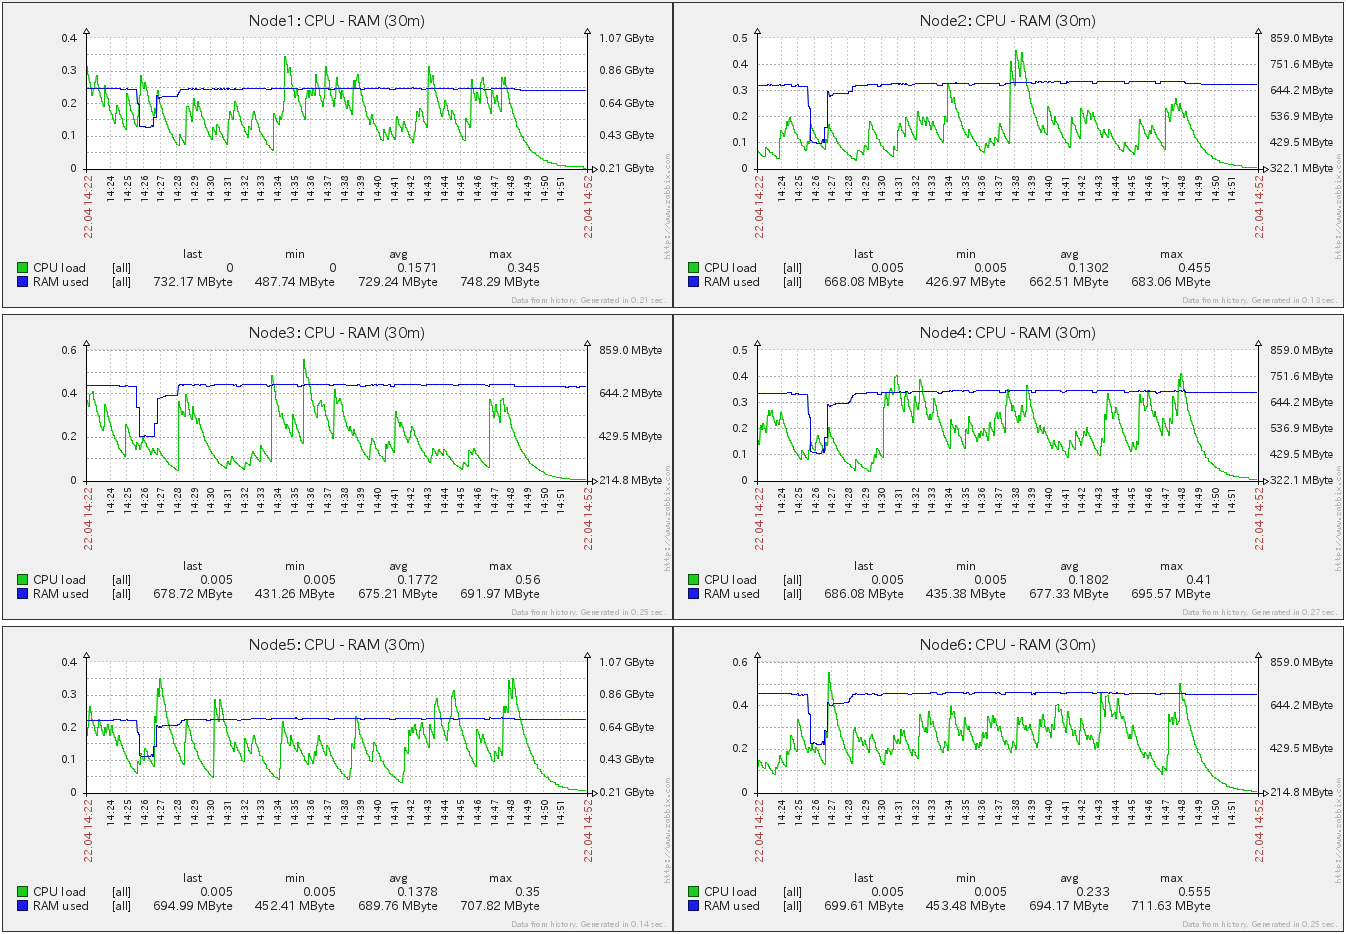
\includegraphics[width=\textwidth]{Testergebnisse/jdbc_aggregation_Testlauf.png}
\caption[Auslastung der Knoten 1 bis 6 im Lasttest der Aggregation]{Auslastung der Knoten 1 bis 6 im Lasttest der Aggregation, 14:28-14:48 Uhr}
\label{fig:auslastungTest1}
\end{figure}
\begin{figure}[h!]
\centering
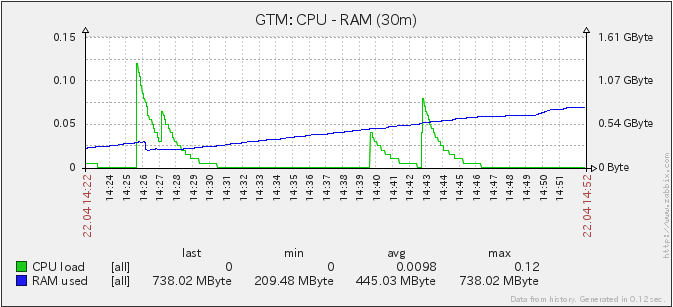
\includegraphics[width=.5\textwidth]{Testergebnisse/jdbc_aggregation_Testlauf_bild2.png}
\caption[Auslastung des Knoten 7 im Lasttest der Aggregation]{Auslastung des Knoten 7 im Lasttest der Aggregation, 14:28-14:48 Uhr}
\label{fig:auslastungTest1_gtm}
\end{figure}


Zusätzlich erfolgt die Aggregation in einem gesonderten Test entsprechend des Anwendungsfalles mit dem \Gls{umn}, mit der Darstellung in Kartenform als Ergebnis.
Dafür wird der \Gls{umn} mit einem Mapfile als \Gls{fcgi} Modul verwendet, siehe Anhang \ref{appendix:mapfileaggregate}.
Das Mapfile stellt Kartenausschnitte der Punktdaten dar und die Karte wird farbig anhand der Metadaten erzeugt.
%Aggregation
%Query vorbereiten   select * from n.nsensorlogs where farmid=1038
%Laufzeitmessung testen   explain analyze
%Auslastung messen/testen    mit Zabbix
%mehrere Durchgänge
%gegenüber stellen
Die Testdefinition baut auf jener aus \cite{ba:kurt} bei Verwendung des \Gls{umn} auf.
Es werden 32 Clients simuliert, indem gleichzeitig 32 Threads in zwei Wiederholungen fünf ausgewählte Kartenbereiche in zufälliger Reihenfolge per WMS abfragen.
Diese Kartenausschnitte enthalten die Einträge aus n.nsensorlogs entsprechend des angeforderten Kartenausschnittes.
Darin wird jeder Wert als Punkt dargestellt und entsprechend des Wertes \verb+applraten+ eingefärbt.
Diese Darstellung wurde aus AgriPort übernommen, färbt die Punkte weiß bis dunkelblau und stellt die Aufnahmemenge von Stickstoff der Pflanzen dar.
Ein Kartenbereich besteht dabei aus fünf Ausschnitten und somit aus fünf WMS Anfragen.
Bei der Erstellung der Kartenausschnitte wurden die aufgeführten fileids berücksichtigt, um eine gleichmäßige Verteilung auf die DataNodes zu erreichen.
Die angeforderten Kartenausschnitte werden als Bilder in den Arbeitsspeicher geladen.

In Vorbereitung des Testes wurde eine sehr hohe Auslastung der CPU in der \Gls{vm} beobachtet, welche die \Gls{umn} Instanz beinhaltet, im Gegensatz zu einer geringen Auslastung der restlichen \Gls{vm}s.
Um einen höheren Durchsatz zu erreichen und das Postgres-XL Cluster mehr auszulasten, wurden der UMN \Gls{vm} zwei weitere CPU Kerne zugeordnet.
Da bereits alle 16 Kerne vergeben sind, wurde die Prozessor Affinität der GTM \Gls{vm} so geändert, dass diese sich ihre zwei Prozessorkerne mit der UMN \Gls{vm} teilt.
Es wurde dafür die GTM \Gls{vm} verwendet, da sie auch bei Benutzung des Postgres-XL Clusters eine geringe CPU Auslastung aufwies\footnote{siehe Abbildung \ref{fig:auslastungTest1_gtm}}.
Diese Ressourcenaufteilung beeinträchtigt die Leistungsfähigkeit des Clusters somit nicht.

%Bilder unteinander setzen: Auslastung, Laufzeiten
%diese auswerten

Die Ergebnisse der Testdurchläufe sind in Tabelle \ref{tbl:ergebnisseTest1UMN} aufgeführt.
Entsprechend der genannten Berechnungsvorschrift ergibt sich eine mittlere Antwortdauer von 2393ms.
\begin{table}[h!]
\centering
%\small
\begin{tabular}{c|c|c}
\textbf{Durchlauf} & \textbf{Durchschnittliche Antwortzeit in ms} & \textbf{Laufzeit des Tests in s} \\ \hline
1 & 2418 & 155 \\ \hline
2 & 2389 & 153 \\ \hline
3 & 2414 & 152 \\ \hline
4 & 2415 & 154 \\ \hline 
5 & 2402 & 152 \\ \hline
6 & 2370 & 153 \\ \hline
7 & 2391 & 152 \\ \hline
8 & 2404 & 154 \\ \hline 
9 & 2380 & 153 \\ \hline
10 & 2394 & 152 \\ \hline
11 & 2375 & 152 \\ 			
\end{tabular}
\caption[Testergebnis Lasttest der Aggregation mit Kartendarstellung]{Testergebnis Lasttest der Aggregation mit Kartendarstellung unter Nutzung des \Gls{umn}}
\label{tbl:ergebnisseTest1UMN}
\end{table}

Die Auslastung aller \Gls{vm}s ist in Abbildung \ref{fig:auslastungTest1UMN} sowie \ref{fig:auslastungTest1UMN_gtm_umn} abgebildet.
In den Knoten eins bis sechs ist zu Beginn eine Erhöhung des genutzten Arbeitsspeichers von etwa 100 MB  zu verzeichnen.
Nach zwei Minuten ändert sich die Auslastung nicht mehr.
Die CPU Auslastung schwankt stark, enthält regelmäßige Leistungsspitzen und ist nicht deckungsgleich zwischen den Knoten.
Dabei befindet sich die Auslastung je nach Knoten zwischen 0.01 und 0.31.
Überblicksartig kann von einer CPU Auslastung 0,1 gesprochen werden.
\begin{figure}[h!]
\centering
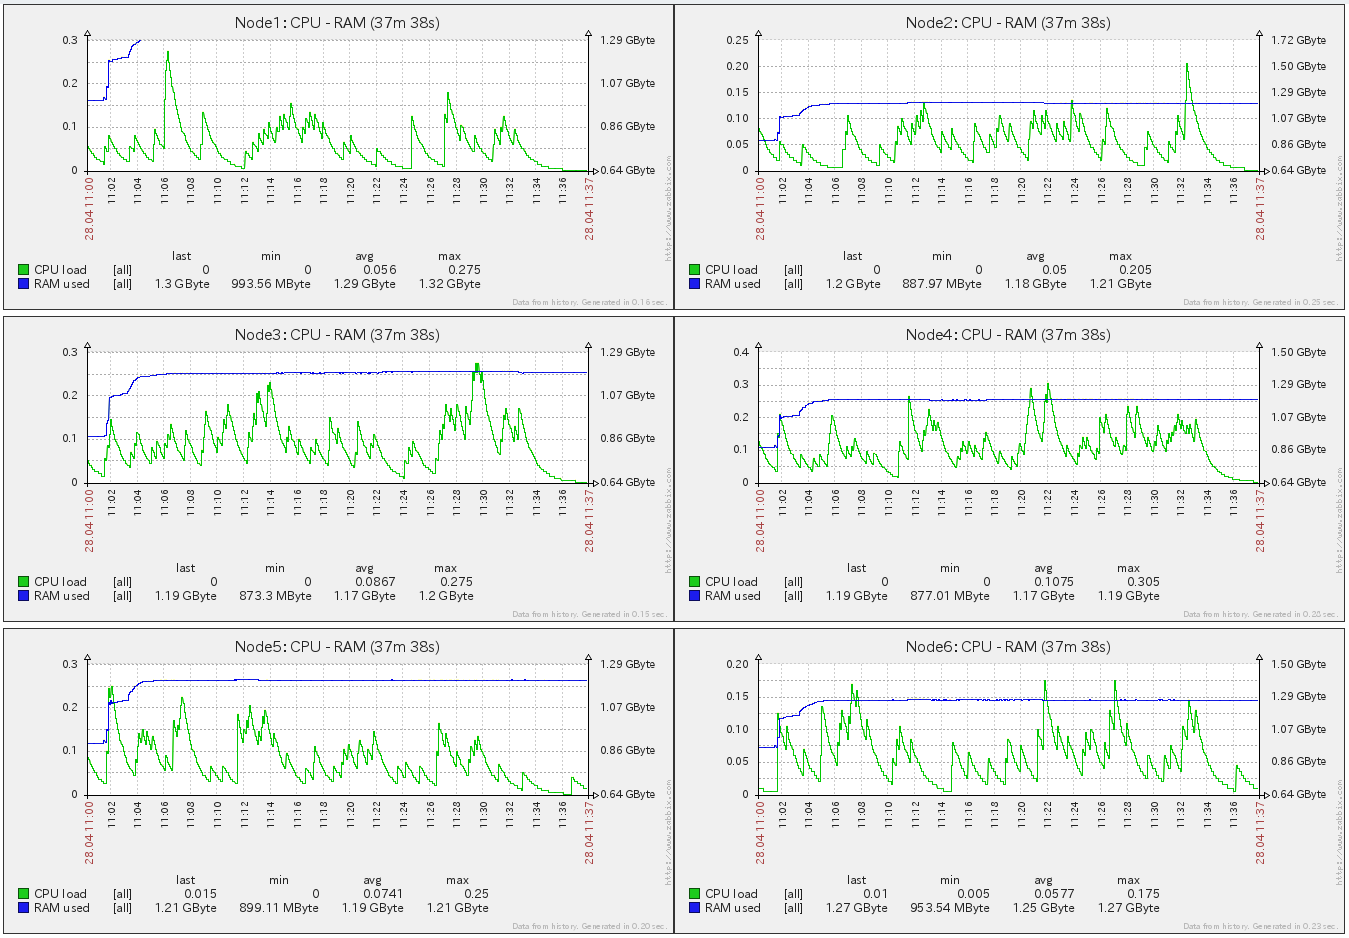
\includegraphics[width=\textwidth]{Testergebnisse/umn_aggregation_Testlauf.png}
\caption[Auslastung der Knoten 1 bis 6 im Lasttest der Aggregation mit Kartendarstellung]{Auslastung der Knoten 1 bis 6 im Lasttest der Aggregation mit Kartendarstellung, 11:03-11:33 Uhr}
\label{fig:auslastungTest1UMN}
\end{figure}
Bezüglich der GTM \Gls{vm} steigt auch in diesem Test die Arbeitsspeicher Auslastung stetig und die CPU Auslastung ist sehr gering.
Der Arbeitsspeicher wird mit etwa 1GB belastet und die CPU wird einzig von 11:15 bis 11:21 Uhr bis zu einem Maximalwert von 0,06 genutzt.
Trotz der Nutzung von vier Prozessoren ist die Auslastung der CPU durch die \Gls{umn} Instanz sehr hoch.
Diese bewegt sich während der Tests zwischen 4.5 und 6.5.
Zu Beginn wird rund 260MB Arbeitsspeicher der \Gls{umn} Instanz zugewiesen, ist zwischen den Tests 40MB niedriger und ansonsten gleich.
\begin{figure}[h!]
\centering
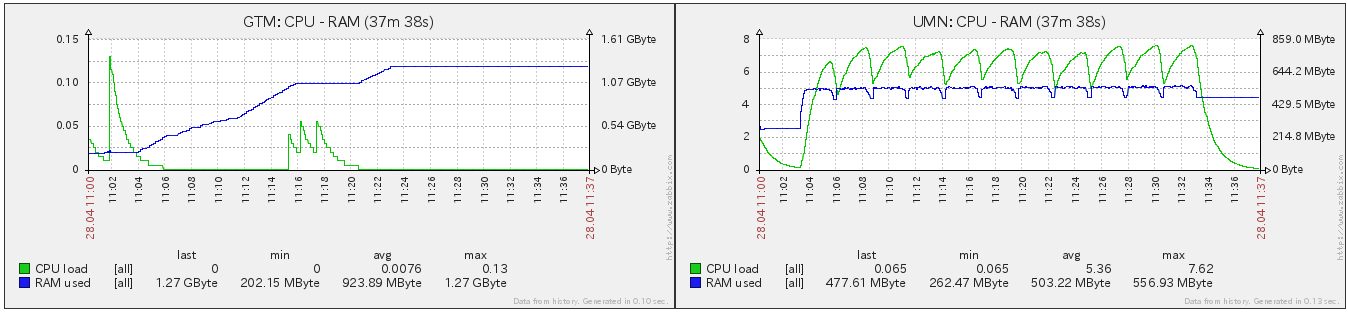
\includegraphics[width=\textwidth]{Testergebnisse/umn_aggregation_Testlauf_bild2.png}
\caption[Auslastung des Knoten 7 im Lasttest der Aggregation mit Kartendarstellung]{Auslastung des Knoten 7 im Lasttest der Aggregation mit Kartendarstellung, 11:03-11:33 Uhr}
\label{fig:auslastungTest1UMN_gtm_umn}
\end{figure}



Für die Lasttests mit der PostgreSQL \Gls{vm} wurden die Datenbankverbindungen zu den Coordinators auf die IP und den Port der PostgreSQL \Gls{vm} geändert.
PostgreSQL und Postgres-XL werden somit mit den gleichen Anfragen in der gleichen Menge belastet.

Die Aggregation mit SQL ergab nach Tabelle \ref{tbl:ergebnisseTest1PG} für die PostgreSQL \Gls{vm} 4319ms durchschnittliche Laufzeit.
\begin{table}[h!]
\centering
%\small
\begin{tabular}{c|c|c}
\textbf{Durchlauf} & \textbf{Durchschnittliche Antwortzeit in ms} & \textbf{Laufzeit des Tests in s} \\ \hline
1 & 4348 & 113 \\ \hline
2 & 4214 & 110 \\ \hline
3 & 4215 & 110 \\ \hline
4 & 4317 & 112 \\ \hline
5 & 4288 & 112 \\ \hline 
6 & 4631 & 122 \\ \hline
7 & 4412 & 116 \\ \hline
8 & 4369 & 114 \\ \hline
9 & 4363 & 114 \\ \hline 
10 & 4154 & 109 \\ \hline
11 & 4226 & 110 \\	
\end{tabular}
\caption[Testergebnis Lasttest der Aggregation mit PostgreSQL \Gls{vm}]{Testergebnis Lasttest der Aggregation mit PostgreSQL \Gls{vm}}
\label{tbl:ergebnisseTest1PG}
\end{table}

Die Auslastung der \Gls{vm} ist in Abbildung \ref{fig:auslastungTest1_pg} abgebildet.
Darin ist zu sehen, dass die Auslastung des Arbeitsspeichers um etwa 180MB zu Beginn des Testdurchlaufes zunahm und nur zwischen den Testschritten temporär um 40MB einbrach.
Weiterhin ist in dieser Abbildung eine bis zu 460 prozentige Auslastung der CPU zu verzeichnen.
Die Auslastung der CPU schwankt zwischen 250\%{} und 460\%{}.
\begin{figure}[h!]
\centering
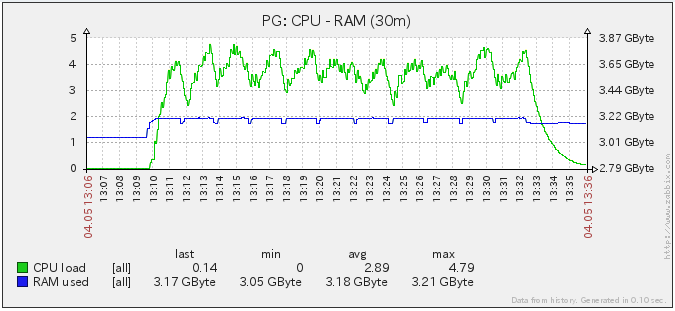
\includegraphics[width=\textwidth]{Testergebnisse/jdbc_aggregation_pg_Testlauf.png}
\caption[Auslastung der PostgreSQL \Gls{vm} im ersten Lasttest]{Auslastung der PostgreSQL \Gls{vm} im Lasttest, 13:09-13:32 Uhr}
\label{fig:auslastungTest1_pg}
\end{figure}


Die Aggregation mit dem \Gls{umn} ergab für die PostgreSQL \Gls{vm} 2595ms durchschnittliche Laufzeit, entsprechend der Tabelle \ref{tbl:ergebnisseTest1PG_UMN}.
\begin{table}[h!]
\centering
%\small
\begin{tabular}{c|c|c}
\textbf{Durchlauf} & \textbf{Durchschnittliche Antwortzeit in ms} & \textbf{Laufzeit des Tests in s} \\ \hline
1 & 2302 & 151 \\ \hline
2 & 2370 & 150 \\ \hline
3 & 2377 & 151 \\ \hline
4 & 2379 & 150 \\ \hline
5 & 2364 & 150 \\ \hline 
6 & 2388 & 150 \\ \hline
7 & 2357 & 150 \\ \hline
8 & 2352 & 150 \\ \hline
9 & 2352 & 150 \\ \hline 
10 & 2348 & 150 \\ \hline
11 & 2365 & 150 \\	
\end{tabular}
\caption[Testergebnis Lasttest der Aggregation mit Kartendarstellung und PostgreSQL \Gls{vm}]{Testergebnis Lasttest der Aggregation mit Kartendarstellung und PostgreSQL \Gls{vm}}
\label{tbl:ergebnisseTest1PG_UMN}
\end{table}

Die Auslastung der PostgreSQL und UMN \Gls{vm} besitzt Ähnlichkeit mit jener der Knoten in Abbildung \ref{fig:auslastungTest1UMN} und \ref{fig:auslastungTest1UMN_gtm_umn}.
Die UMN \Gls{vm} wird bezüglich der CPU um ein Vielfaches der Kapazität belastet.
Die Auslastung beträgt 165MB bis 270MB der Arbeitsspeichers und 450\%{} bis 680\%{} der CPU.
\begin{figure}[h!]
\centering
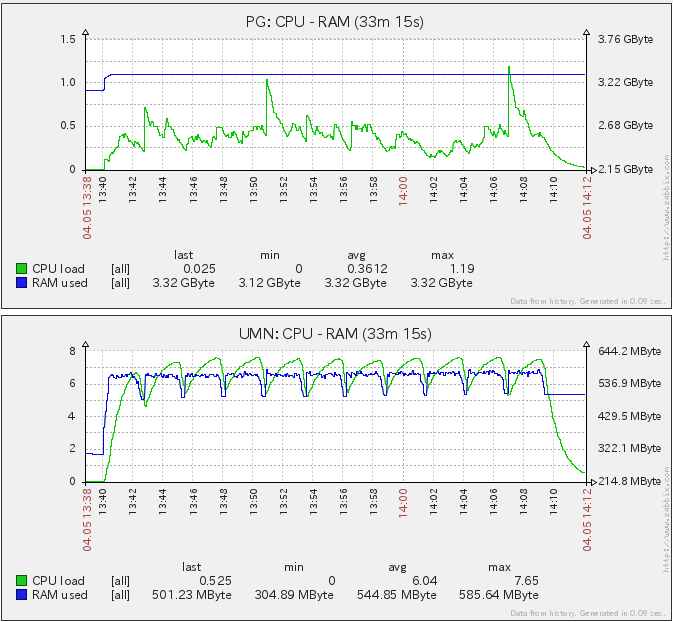
\includegraphics[width=\textwidth]{Testergebnisse/umn_aggregation_pg_Testlauf.png}
\caption[Auslastung der PostgreSQL \Gls{vm} im Lasttest der Aggregation mit Kartendarstellung]{Auslastung der PostgreSQL \Gls{vm} im Lasttest der Aggregation mit Kartendarstellung, 13:40-14:09 Uhr}
\label{fig:auslastungTest1UMN_pg}
\end{figure}





\subsection{Verarbeitung}
Der Lasttest zum messen der Verarbeitungsleistung ruft die SQL Funktion\\
\textit{nutrients.contouringcorrectedatop(integer)} auf.
Diese führt den speziellen Kriging Algorithmus anhand der übergebenen fileid mit den Werten in nutrients.samples durch.
Es werden fileids aus der Tabelle \ref{tbl:entrysnsamples} verwendet.
\begin{table}[h!]
\centering
%\small
\begin{tabular}{c|c|c|c}
\textbf{fileid} & \textbf{Anzahl Einträge} & \textbf{Betroffener Knoten} & \textbf{Betroffener DataNode} \\ \hline
4004 & 494 & 3 & 6 \\ \hline	%dn 6    
3110 & 404 & 6 & 11 \\ \hline	%dn 11    geht nicht
3114 & 369 & 2 & 4 \\ \hline	%dn 4
%3904 & 260 & 1 & 2 \\ \hline	%dn 2
%742 & 201 & 4 & 8 \\ \hline		%dn 8
%4204 & 197 & 1 & 2 \\ \hline	%dn 2
4186 & 160 & 4 & 8 \\ \hline	%dn 8
5796 & 143 & 1 & 1 \\ \hline	%dn 1
5915 & 110 & 5 & 9 \\ %\hline	%dn 9
%5050 & 12 & 4 & 8 \\
\end{tabular}
\caption{Anzahl der Einträge in nutrients.samples nach fileid}
\label{tbl:entrysnsamples}
\end{table}	%Verteilung der Daten nicht so wichtig - da ids mit vielen Einträgen zum Abbruch führen muss es so gehen
Neben der Laufzeit ist gesondert die Auslastung der einzelnen Knoten zu beobachten und zu bewerten.
Zu Beginn dieser Untersuchung steht nicht fest, in wie weit die DataNodes mit in die Berechnungen der Coordinator mit einbezogen werden.
%Nur Coordinator scheint zu berechnen - dies ist mit auslastung EINES Coordinator zu beweisen
Eine automatisierte Verteilung der Berechnungen ist für einen höheren Durchsatz wünschenswert.
%mehrere Aufrufe gleichzeitig - mit scala?

Es zeigte sich, dass mit Postgres-XL zwar Daten per SQL \textit{Insert into} gespeichert werden können, es jedoch bei einer Speicherung innerhalb einer SQL Funktion zu Fehlern kommt.
In der Fehlermeldung wird auf unbekannte Parameter verwiesen, obwohl alle Daten in Parametern korrekt sind.
Aus diesem Grund wurden Nebenwirkungen der Funktionen der Berechnungen entfernt, sodass zwar alle Berechnungen durchgeführt werden, die Ergebnisse aber nicht verfügbar sind.
Weiterhin zeigte sich, dass Funktionen welche die Erweiterung plr für die Nutzung der Sprache R verwenden, zufällige Fehler werfen.
Die Wahrscheinlichkeit des Auftretens des Fehlers konnte durch neu laden der verwendeten R Bibliotheken bei jedem Funktionsaufruf veringert werden.
So wird\\\verb+nutrients.contouringcorrectedatop(integer)+ ohne Nebenwirkungen ausgeführt.

Die Testdefinition wurde aus dem Leistungstest der Aggregation übernommen.
Geändert wurde dabei die SQL Anfrage und die Anzahl der Anfragen an Postgres-XL.
Pro Coordinator wird gleichzeitig die Interpolation von sechs fileids aufgerufen.
Diese Definition ist jedoch nicht verwendbar, da bei gleichzeitigen parallelen Aufruf Fehler geworfen werden.
Dabei verlieren die Coordinator die Verbindung zu den DataNodes.
Aus diesem Grund wird ein Coordinator verwendet und die Anfragen erfolgen sequenziell mit den fileids aus Tabelle \ref{tbl:entrysnsamples} beginnend mit dem ersten Eintrag.

%Nur einen Coordinator ansprechen und Auslastung beobachten
% Auslastungen als Bilder in Anhang und darauf verweisen
% nur coodinator scheint augelastet zu werden - bewerten

%Bilder unteinander setzen: Auslastung, Laufzeiten
% diese auswerten
% auf Fehleranteil eingehen
Dieser Lasttest hat eine durchschnittliche Laufzeit von 975s im Postgres-XL Cluster.
Tabelle \ref{tbl:ergebnisseTest2} enthält die einzelnen Laufzeiten und die maximale und minimale Antwortzeit der Anfragen.
Die durchschnittliche Antwortzeit wird nicht aufgeführt, da 6 Anfragen gestellt werden, der Durchschnitt somit leicht berechenbar ist, und sich die Laufzeiten der Berechnungen bis zum 20 fachen unterscheiden.
Die Laufzeit der Anfragen ist direkt proportional Abhängig zur Anzahl der betroffenen Einträge in nutrients.samples.
\begin{table}[h!]
\centering
%\small
\begin{tabular}{c|C{3.4cm}|C{3.4cm}|c}
\textbf{Durchlauf} & \textbf{Maximale Antwortzeit in ms} & \textbf{Minimale Antwortzeit in ms} & \textbf{Laufzeit des Tests in s} \\ \hline
1 & 563130 & 24992 & 987 \\ \hline
2 & 553914 & 24948 & 978 \\ \hline
3 & 552416 & 25027 & 970 \\ \hline
4 & 551919 & 25097 & 970 \\ \hline
5 & 553892 & 24919 & 977 \\ \hline 
6 & 552905 & 25108 & 971 \\ \hline
7 & 553884 & 24985 & 977 \\ \hline
8 & 553931 & 24843 & 976 \\ \hline
9 & 554989 & 24947 & 979 \\ \hline 
10 & 554304 & 24916 & 978 \\ \hline
11 & 552536 & 24915 & 975 \\	
\end{tabular}
\caption[Testergebnis Lasttest der Verarbeitung]{Testergebnis Lasttest der Verarbeitung}
\label{tbl:ergebnisseTest2}
\end{table}

Abbildung \ref{fig:auslastungTest2} zeigt eine durchgehend starke Auslastung des ersten Knoten\footnote{Knoten eins wurde im Test angesprochen.} im Gegensatz zu einer geringen Auslastung der restlichen Knoten.
Knoten eins, in Abbildung Node1 genannt, verwendet für die Testreihe 400MB und für einen Testdurchlauf etwa 100MB Arbeitsspeicher.
Die Auslastung der CPU bewegt sich während der Testreihe zwischen 33\%{} und 78\%{}.
Die restlichen Knoten reservierten während des Testlaufes stetig Arbeisspeicher, bis zu 100MB pro Knoten.
Bezüglich der CPU kann von einer nicht relevanten Auslastung ausgegangen werden.
Zwar existieren bei jedem Knoten Leistungsspitzen bis zu 80\%{}, jedoch dauert eine solche Auslastung maximal 5 Minuten und das Auftreten dieser Spitzenwerte ist während der Testreihe unterschiedlich sowie nicht deckungsgleich zwischen den Knoten.
\begin{figure}[h!]
\centering
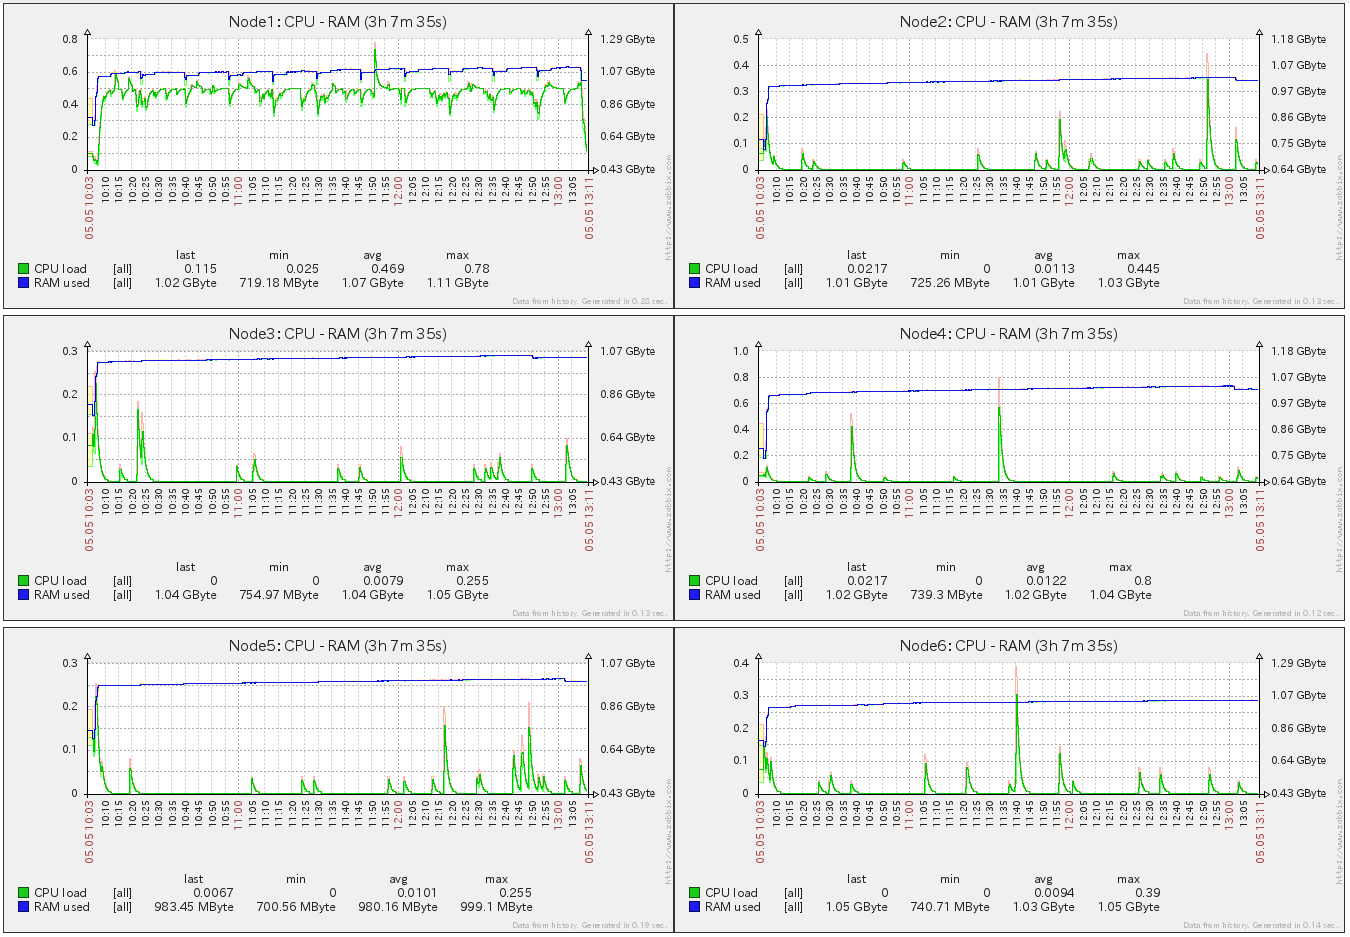
\includegraphics[width=\textwidth]{Testergebnisse/jdbc_contouring_Testlauf.png}
\caption[Auslastung der Knoten 1 bis 6 im Lasttest der Verarbeitung]{Auslastung der Knoten 1 bis 6 im Lasttest der Verarbeitung, 10:07-13:09 Uhr}
\label{fig:auslastungTest2}
\end{figure}
Der Knoten sieben zeigt erneut eine charakteristische geringe Auslastung der CPU sowie einer steigenden Auslastung des Arbeitsspeichers, wie in Abbildung \ref{fig:auslastungTest2_gtm} zu sehen.
So wird etwa 1 GB verwendet, zusätzlich vom Grundwert von 610MB.
\begin{figure}[h!]
\centering
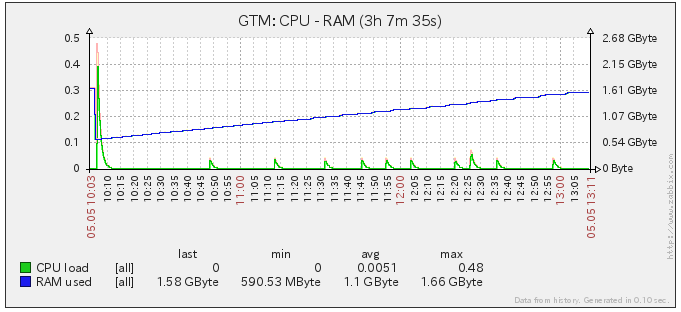
\includegraphics[width=\textwidth]{Testergebnisse/jdbc_contouring_Testlauf_bild2.png}
\caption[Auslastung des Knoten 7 im Lasttest der Verarbeitung]{Auslastung des Knoten 7 im Lasttest der Verarbeitung, 10:07-13:09 Uhr}
\label{fig:auslastungTest2_gtm}
\end{figure}

%mit SQL Bordmitteln - pg_bench eventuell zusätzlich um ein paar Aussagen zum cluster overhead zu treffen

%PostgreSQL System nicht vergessen!
